% Red-Teaming Semantic Entropy. An arXiv preprint.
%
% TYPOGRAPHY, chosen by measuring the two nearest papers in this literature rather than
% by taste. Both were downloaded and measured on 2026-08-30:
%   Kuhn et al.   (arXiv 2302.09664v3, 19pp): text block 396pt = 5.50in, side margins
%                 108/108pt, body face Nimbus Roman (Times) at 9.96pt, leading ~11pt.
%   Kossen et al. (arXiv 2406.15927v1, 22pp): text block 398pt = 5.53in, side margins
%                 107/106pt, body face Nimbus Roman (Times) at 9.96pt, leading ~11pt.
% Both are the single-column NeurIPS/ICLR preprint measure. We adopt it.
%
% WHY THE FONT AND THE MEASURE MOVED TOGETHER. Measured characters per full line:
% Kuhn 97, Kossen 98, and this paper 96 at its old 6.5in/11pt Computer Modern setting.
% The old measure was therefore NOT over-long in characters, which is the quantity that
% governs reading comfort. Narrowing to 5.5in while keeping 11pt Computer Modern would
% have driven it DOWN to about 81 and made the paper look unlike its neighbours in the
% other direction. Times is a narrower face, which is exactly how Kuhn and Kossen fit
% 97 characters into 5.5in. Changing one without the other misses on either side.
\documentclass[10pt,letterpaper]{article}

\usepackage[utf8]{inputenc}
\usepackage[T1]{fontenc}

% BODY FACE. Times for text, Computer Modern for math: this is what both reference papers
% do (their font tables carry NimbusRomNo9L for text alongside CMMI/CMSY/CMEX for math).
% It also fixes a real defect. Under [T1]{fontenc} with Computer Modern and no cm-super
% installed in this TeX Live, every body glyph was shipped as a Type 3 BITMAP: the old
% main.pdf carried 17 Type 3 fonts and rendered fuzzy at any zoom. Times (ptm) has genuine
% Type 1 outlines in T1, so the body text is now vector.
\usepackage{times}
% times.sty would also route \texttt to Courier, which is very wide. Latin Modern Mono has
% real T1 Type 1 outlines and is narrower, so \texttt stays vector without the Courier bulk.
\renewcommand{\ttdefault}{lmtt}

\usepackage{amsmath,amssymb}
\usepackage{graphicx}
% figures/ lives at the repo root; accept a build launched from either the root or paper/.
\graphicspath{{../figures/}{figures/}}
\usepackage{booktabs}

% Caption label in bold, as in both reference papers. Deliberately NO font= option: the
% table environments in sections/ set \footnotesize BEFORE \caption, so the captions
% already inherit a reduced size, and naming a size here would silently ENLARGE them.
\usepackage[labelfont=bf,skip=6pt]{caption}
% Figure captions at \small, as in both reference papers. Scoped to [figure] on purpose:
% the FIGURE captions in sections/ render at full body size and are long (about 960 and
% 1050 characters), whereas the TABLE captions already sit inside a ootnotesize group, so
% an unscoped font= would have ENLARGED them. This also buys the vertical room that lets
% fig_floor_budget be placed at all: at 10pt it overshot the column by 1.41pt and was
% therefore deferred to the end of the document.
\captionsetup[figure]{font=small}

\usepackage[letterpaper,left=1.5in,right=1.5in,top=1in,bottom=1in]{geometry}

% FLOAT PLACEMENT. Every float in this paper is declared [t]. LaTeX's default \topfraction
% of 0.7 forbids a top float taller than 70% of the column, so the large ones could never
% be placed and were deferred to the end of the document, which is the "tables stranded on
% their own pages" the author reported. These are the standard relaxations.
\setcounter{topnumber}{3}
\setcounter{bottomnumber}{2}
\setcounter{totalnumber}{4}
\renewcommand{\topfraction}{0.9}
\renewcommand{\bottomfraction}{0.8}
\renewcommand{\textfraction}{0.07}
\renewcommand{\floatpagefraction}{0.75}

% sort&compress so that a multiple citation prints as [5, 10] rather than [10, 5],
% and collapses runs to [5-7].
\usepackage[numbers,sort&compress]{natbib}

\usepackage{xcolor}
\definecolor{refblue}{RGB}{0,64,128}
\definecolor{citeblue}{RGB}{0,96,112}
\usepackage[colorlinks=true,linkcolor=refblue,citecolor=citeblue,urlcolor=refblue,
            breaklinks=true]{hyperref}

% microtype: verified present at
% /usr/share/texlive/texmf-dist/tex/latex/microtype/microtype.sty. Character protrusion and
% font expansion are what stop justified Times from gaping at this measure.
\usepackage[protrusion=true,expansion=true,final]{microtype}

% Working title. It avoids collision with "Adversarial Paraphrasing" (2506.07001).
% PROPOSED Option-B title (protocol-led); the attack-led original is kept below, commented.
\title{\bfseries Crying Wolf, Carefully: What It Takes to Evaluate Paraphrase Attacks on
Sampling-Based Hallucination Detectors}
% \title{Crying Wolf: Meaning-Preserving Paraphrases Break Sampling-Based
% Hallucination Detectors in Both Directions}   % attack-led (Option A) original

% AUTHOR AND DATE BLOCK.
% Affiliation is still intentionally omitted for the preprint; fill before any external
% posting. It is deliberately NOT invented here, and no contact address is printed.
% \date{\today} used to stamp the compile date into the paper, so the PDF claimed whatever
% day it happened to be built. arXiv applies its own datestamp, so no date is typeset;
% the slot carries the document's status instead, which is what keeps the block from
% reading as unfinished.
\author{ScriptSampler}
\date{\normalsize Preprint}
\begin{document}
\maketitle

\begin{abstract}
% ABSTRACT LENGTH BUDGET. arXiv's abstract field takes 1920 characters.
% NOW: 308 words / 1918 characters, counted 2026-08-31 by the rule below. 2 to spare.
%
% THE SINGULAR "the qualifier" WAS FIXED ON 2026-08-31, AND IT COST 3. Once the clusterer
% scope landed (see the next block), the Abstract carried TWO scope qualifiers on the floor
% sentence pair, "Under NLI clustering" and "At that standard N=10", and still said "the
% qualifier is load-bearing", singular, naming neither. Discussion and Conclusion had both
% been updated to carry two: discussion.tex already said "Both qualifiers are load-bearing"
% of exactly this pair (right after "At N=10, and under the DeBERTa-large-MNLI clustering"),
% and conclusion.tex names the budget, then "A second qualifier is load-bearing in the same
% way, and it names the clusterer rather than the budget". Grep the sentences, not line
% numbers: the ones this comment used to carry had already rotted by seven and twenty-three
% lines. "the qualifier is" (16) -> "both qualifiers are" (19) is the whole change, and the
% Abstract now uses the Discussion's own sentence verbatim, so the three files agree.
% NAMING THEM WAS COSTED AND DOES NOT FIT. "the budget and the clusterer are load-bearing"
% is 45 against the 28 of "the qualifier is load-bearing", which is +17 into 5. The
% compressed form is the same trade the clusterer scope itself makes below: the Abstract
% names the count, the body names the two. If characters ever free up, this is the THIRD
% thing to buy, after the two-orders-of-magnitude gloss and the DeBERTa checkpoint name.
%
% THE ORACLE SCOPE QUALIFIER WAS ADDED AT ZERO NET COST on 2026-08-30, and this is the
% record of what paid for it. The adjudication of that date (results/gemini_adjudication_
% 2026_08_30.md, item M1) established that the floor is a fact about the EQUIVALENCE
% RELATION as much as about the model: Table 1 prints the same estimand on the same 80
% targets at 46.2% (exact match), 10.0% (NLI) and 1.2% (judge), and the exact and NLI
% Wilson intervals do not overlap. An unscoped 10.5% is therefore not a claim about "the
% detector", it is a claim about the detector's NLI clusterer. "Under NLI clustering "
% (21) was inserted ahead of the 10.5%, keeping the rate and its "1424 clean correct"
% label in ONE sentence, which is what the proximity guard cares about. Three rewordings
% paid for it exactly, and none of them dropped a clause, number, interval, qualifier or
% concession:
%   (1) PAID 11. "Every threshold above the maximum flags nothing" -> "No threshold above
%       the maximum fires". Same proposition; "fires" is already the paper's own verb for
%       this ("the only threshold that honours it never fires", "the cheapest threshold
%       that fires at all"), so the swap also removes a synonym.
%   (2) PAID 5. "The atom is empty, and the obstruction goes with it." -> "...and the
%       obstruction with it." Ellipsis only. "it" still sits in the same sentence as the
%       atom it refers to, which is the property note (2) below was written to protect.
%   (3) PAID 5. "What 200 answers cannot then do" -> "What 200 answers cannot do". A
%       connective, carrying nothing.
% Do NOT spend these three again: they are already spent, and the abstract is back at 5.
% The scope qualifier is now covered by the WHAT MAY NOT BE TRIMMED rule below.
%
% NO EM DASHES, ANYWHERE IN THIS FILE, IN ANY SPELLING. Not the three-hyphen LaTeX form,
% not a literal U+2014, not a two-hyphen stand-in doing an em dash's job. On 2026-08-30 the
% file held seven of the first kind and thirteen of the third; it holds none of either now.
% The seven were three in the Abstract, two in the title comments at the top of the file,
% and two in THE RULE below; the thirteen were all in these comments. Do not reintroduce
% one, in the Abstract or in a comment.
%
% Was 302 words / 1909 characters (11 to spare) until 2026-08-30, when the Abstract's three
% were restructured away. Net cost 6 characters, and nothing was dropped to pay for them:
% no clause, no number, no interval, no qualifier, no concession. Only sentence shape
% changed, at three sites, and two of the three paid for the first.
%  (1) COST 9. The appositive gloss on the floor became its own sentence: "...mutually
%      distinct meanings. That is 10.5% [9.0, 12.2] on 1424 clean correct answers." A
%      relative clause ("..., which is 10.5%") was one character dearer and read worse,
%      and "That chance is" was seven dearer. The 10.5% and its "1424 clean correct" label
%      stay in ONE sentence, which is what the proximity guard cares about.
%  (2) PAID BACK 2. The aside inside the N=40 sentence was promoted to the main clause and
%      the conclusion split off behind it: "At N=40 none of the fair pool's 200 correct
%      answers reaches ln 40 (0/200, at most 1.9%). The atom is empty, and the obstruction
%      goes with it." The pinned literal "(0/200, at most 1.9%)" and the label "the fair
%      pool's 200 correct answers" stay in ONE sentence, and "it" now sits in the same
%      sentence as the atom it refers to. Keeping the old "Running the fair pool's 200
%      correct answers to N=40 empties the atom" as the lead sentence instead cost 1 and
%      left "it" pointing back across a sentence break, so it was declined.
%  (3) PAID BACK 1. The 5%-budget sentence was cut in two at "which we report as".
% Was 299 words / 1897 characters (23 to spare) until 2026-08-29, when the closing sentence
% changed from "The confirmatory evaluation is under way" to the landed result. That cost 12
% characters and nothing was dropped to pay for it: no clause, number, interval, qualifier
% or concession. Longer candidates naming the null explicitly were costed and declined at 1
% to 4 characters of remaining margin.
% Was 321 words / 2020 characters (over by 100) until the 2026-08-26 work; ~215 words on
% 2026-08-19, ~200 at the critic gate of 2026-08-13. That work was two passes. Pass 1 was
% pure prose economy. It made 19 rewordings worth 127 characters and dropped no clause,
% number, interval, qualifier or concession. Pass 2 replaced the floor sentence with the
% non-identification wording below and paid for it by spending the gloss "so about half of
% an uncorrected result is selection on sampling noise" (69), which was redundant against
% the 44% [23%, 64%] it restated. The one large candidate still unspent is the
% self-referential "; both qualifiers are load-bearing" (34, and 31 in the singular form it
% carried until 2026-08-31). DO NOT spend it here alone: the same phrase is live in
% discussion.tex and conclusion.tex, so dropping it from this
% file only would leave the paper disagreeing with itself, which is the defect class of
% critique_log 37/38. Spend it in all three or in none.
%
% THE RULE, written out because this comment twice said "the same rule" and never named it.
% Count what sits between this environment's begin and end lines. Those two lines are markup
% and do NOT count. Drop these comment lines. Replace every macro by what it RENDERS
% (\emph{x} -> x, $N{=}10$ -> N=10, \% -> %, \ln -> ln, $ deleted). Collapse runs of
% whitespace to a single space. A newline in this file becomes one space in the arXiv field,
% so the line wrapping here costs nothing. But PASTE THE RENDERED TEXT, not this source.
% Pasted with {=} left intact, the same abstract is 1921, one character OVER the cap and
% rejected. The old figure here said 1905 and called it a fit; it was wrong on both counts
% and it was wrong for the 1909-character Abstract too, which measured 1921 the same way.
% Recount before believing any number above.
%
% WHAT MAY NOT BE TRIMMED. Each of these was bought with a withdrawn claim:
%  - EVERY INTERVAL. Quoting a rate without one is this project's named failure mode.
%  - EVERY SCOPE QUALIFIER. "At that standard N=10" is the difference between a correct
%    claim and a retracted one. The 5%-budget claim is true at N=10 and false at N=40, and
%    the paper concedes that. "discrete" scopes the estimator: the result does not
%    transfer to the likelihood-weighted Eq.(5) variant its authors call their main method.
%    "Under NLI clustering" scopes the RELATION, and it is the newest of the three and the
%    one most likely to be trimmed by someone who reads it as filler. It is not filler. On
%    the same 80 targets the at-cap rate is 46.2% under exact match and 1.2% under the
%    judge, so the unscoped sentence would be asserting a property of "semantic entropy"
%    that three defensible clusterings do not agree on, across a range that straddles the
%    5% line the very next sentence rules out. That is the same defect class as the two
%    retracted sentences below: a claim true on one branch, printed as if unconditional.
%    THE ABSTRACT'S FORM IS THE COMPRESSED ONE, AND DELIBERATELY. The canonical scoped form
%    the rest of the paper carries is "at N=10, under bidirectional DeBERTa-large-MNLI
%    clustering" (discussion.tex, limitations.tex, introduction.tex, conclusion.tex). Naming
%    the model here costs 8 characters over "Under NLI clustering" and there are 5, so the
%    Abstract names the relation family and the body names the checkpoint. If characters
%    ever free up, lengthening this is the SECOND thing to buy; the first is still the
%    two-orders-of-magnitude gloss listed further down.
%  - THE N=40 CONCESSION. The claim is that the OBSTRUCTION is gone, never that some
%    interval clears 5%. Do NOT reinstate an interval on the 2.0% floor. The reason is NOT
%    that the two candidate intervals were imprecise; it is that the quantity a reader
%    would take the interval to describe is NOT IDENTIFIED at n=200. That quantity is the
%    population mass at the top of support, which is what "the floor" means to an operator
%    who could see the whole population. It equals 2.0% if the population can never yield 39
%    distinct meanings in 40, and can be arbitrarily smaller if it can; 0/200 is the modal
%    outcome under both branches and the sample cannot choose between them. This argument
%    is model-free (results/n40_floor_estimator_ruling.md sections 1 and 13); the coverage
%    simulation quantifies one branch and is not the reason.
%
%    TWO SENTENCES ARE RETRACTED BY NAME. Neither may come back, in this file or any other:
%     (i) that the 2.0% "is the resolution of the pool and not a property of the detector".
%         Ruling section 2, verbatim: "Do not print that sentence." It is true only in
%         the second branch. In the first, 2.0% estimates a real population quantity and
%         section 8 measures Wilson's coverage there at 95.06%. It was in this Abstract
%         until 2026-08-26 and a prose sweep caught it; it is not a stylistic variant of
%         the sentence now printed, it is the claim that one was written to replace.
%     (ii) that "the estimand dissolves once the ceiling atom empties". Ruling section 13,
%         "What does not survive". A branch-conditional claim dressed as an unconditional
%         one. It was in THIS COMMENT until 2026-08-26, which is worse than being in the
%         body: a comment instructs the next editor, so it does not merely record an error,
%         it schedules one.
%
%    Omitted from the Abstract for BUDGET ONLY, and load-bearing in the Discussion: the two
%    admissible readings differ by more than two orders of magnitude, which is why the row
%    gets no interval rather than a wide one. Do not read its absence here as doubt about
%    it, and restore it first if characters ever free up.
%  - "we claim no attack effect here". THE RUN IS NO LONGER PENDING. It completed 80/80 on
%    2026-08-29 03:57 (results/null_control_report_defb.md), so this clause is now a
%    MEASURED NON-REJECTION and not a placeholder: the pre-committed randomised-tie
%    exceedance test gives p = 0.939 (NLI), 1.000 (exact), 1.000 (judge) at n=77. Those are
%    medians over 101 tie-break draws. Keep the clause. Do NOT restore any "under way", "is
%    running", "pending" or "should the effect survive" wording anywhere in the paper; six
%    such sites across five files were cleared on 2026-08-29 and the whole point of listing
%    this here is that a comment does not merely record an error, it schedules one.
%
%    WHY THE NON-REJECTION SURVIVES, AND WHY IT IS NOT THE REASON THIS COMMENT USED TO
%    GIVE. Until 2026-08-30 this bullet asserted that "the median observed exceedance total
%    sits ABOVE its null expectation in every arm, the direction against the attack", and
%    that "no draw in any arm reaches 0.05". BOTH ARE CONDITIONAL ON A = 181 AND NEITHER
%    MAY BE RESTORED. A is the search budget the null prices in, and the adjudication of
%    2026-08-30 (section 2) established from src/se/attacks/optimizer.py that the maximum
%    ranges over the FEASIBLE candidates only, that the feasibility gate is applied lazily
%    so just 4703 of 14,400 scored children were ever checked, and that A is therefore NOT
%    IDENTIFIED from anything the run recorded. Over the admissible range the NLI arm's
%    median p runs from below 0.001 at A = 41 to 0.939 at A = 181 and crosses 0.05 near
%    A = 90, which is inside that range. Those three figures are the SHIPPED
%    implementation's, and they are the ones experiments.tex prints; until 2026-08-31 this
%    bullet said "to 0.92" and "at about A = 92", which came from an adjudicator's
%    independent reimplementation under a different tie RNG. At A = 89 the shipped code
%    gives a median p of 0.0459 and at A = 90 it gives 0.0512, so 90 is the crossing and 92
%    is not. Do not restore either figure: a comment does not merely record an error, it
%    schedules one, and this one had scheduled a body edit away from a number the paper
%    measures. The exceedance-direction claim is false for NLI at the low end.
%    What carries the headline instead is that the PRE-REGISTERED ADJUDICATOR ARM IS
%    INVARIANT: the judge's median p is 1.000 at every A from 41 to 181, and so is exact
%    match's. That is the defence the paper now makes, at introduction.tex and
%    conclusion.tex. The Abstract states the non-rejection without printing a p-value or a
%    draw count, so it needs no repair; do not add one back to buy emphasis.
%  - The literal "($0/200$, at most $1.9\%$)" is pinned by
%    scripts/derived_paper_quantities.py, and the population labels "1424 clean correct"
%    and "the fair pool's 200 correct answers" by scripts/check_population_labels.py.
%    Reword either and a green suite goes red; that is the guard working, not a stale pin.
%
% Everything cut from here over the rounds is still stated where it belongs: the
% three-estimator scoping and the Eq.(4)/Eq.(5) transfer argument in Methods, the N=20
% pilot in Discussion, the judge validation in Methods, the interval on every rate in
% Discussion and Conclusion.
Sampling-based hallucination detectors such as semantic entropy are deployed on a claim of
phrasing-invariant uncertainty. We tried to break it with meaning-preserving paraphrases and
found the binding constraint falls on the operator, not the attacker. The \emph{discrete}
estimator we study weights meaning clusters by sample counts, so it is the entropy of a
partition of $N$: at the standard $N{=}10$ it takes $39$ values, with an atom at the maximum.
No threshold above the maximum fires, so while the atom carries mass the lowest
false-alarm rate a firing threshold can have \emph{is} the chance a clean correct answer
yields $N$ mutually distinct meanings. Under NLI clustering that is $10.5\%$ [$9.0$, $12.2$]
on $1424$ clean correct answers. At that standard $N{=}10$ an operator cannot have a $5\%$
false-alarm budget, however well the score ranks; both qualifiers are load-bearing. At $N{=}40$
none of the fair pool's $200$ correct answers reaches $\ln 40$ ($0/200$, at most $1.9\%$). The
atom is empty, and the obstruction with it. What $200$ answers cannot do is locate the
floor: their cheapest alarm costs $2.0\%$, but that is the population's floor only if it can
never yield $39$ distinct meanings in $40$, a question $200$ answers cannot settle, so we
quote no interval. The threshold honouring a $5\%$ budget achieves
$5.0\%$ [$2.7$, $9.0$] on the same $200$ answers. We report that as a measured operating
point, not a demonstration that one at or below $5\%$ exists. Measuring an attack here needs
stronger controls than the literature's random-perturbation baseline: re-scoring each
selected paraphrase on an independent sample retains only $44\%$ [$23\%$, $64\%$] of the
apparent effect. Our
protocol makes it answerable: score-independent target selection, an answer-invariance
success criterion, a null priced against the attacker's search budget, and an independent
LLM-judge equivalence oracle. The confirmatory run is complete and does not reject; we claim
no attack effect here.
\end{abstract}

\section{Introduction}
% Introduction. Motivation and contributions are stable. The null-controlled headline
% landed on 2026-08-29 and its figures are live in the text below.
%
% THE PROVENANCE STORY IS LOAD-BEARING AND WAS BEING RETRACTED HERE. Until 2026-08-30
% contribution (1) opened "A measurement-validity result about discrete semantic entropy,
% INDEPENDENT OF WHETHER ANY ATTACK SUCCEEDS". That clause is logically true and narratively
% fatal: the Abstract's one-line provenance ("We tried to break it with meaning-preserving
% paraphrases and found the binding constraint falls on the operator, not the attacker")
% asserts a causal link between the attack work and the headline, and the clause severs it,
% leaving two unrelated papers stapled together. An external reviewer finished the 34-page
% draft still asking why the paper is framed around the lattice rather than around the
% clustering model's weaknesses, which is a referee reporting that the pivot did not land
% (results/gemini_adjudication_2026_08_30.md section 6). Three changes answer it and they
% work only together; do not revert one of them alone.
%   (a) The clause now reads "which the attack investigation uncovered and which stands
%       whether or not any attack succeeds". Same logical content, opposite narrative effect.
%   (b) A bridging paragraph before \paragraph{Contributions.} says how the controls produced
%       the finding: a null that must stay valid under ties at the cap forces you to
%       characterise the cap, and characterising the cap IS the measurement-validity result.
%   (c) The third paragraph names the pivot at line ~35 instead of leaving it until the
%       contributions list. Sixty-eight lines of attack setup was too long to hold a reader
%       on the wrong prior about what they were reading.
%
% TWO CLAIMS ABOUT THE EXCEEDANCE TEST WERE DELETED HERE ON 2026-08-30 AND MAY NOT RETURN:
% that "no draw in any arm reaches the 5% cut", and that "the observed exceedance count sits
% ABOVE its null expectation in all three, which is the direction against the attack". Both
% hold only at A = 181, A is an upper bound rather than a measurement, and the shared-NLI
% arm's p crosses 0.05 inside the admissible range. experiments.tex carries the range, the
% sensitivity rows and the arithmetic; this file states the consequence only, which is that
% the non-rejection is rested on the pre-registered adjudicator arm because that arm is the
% one invariant to the unidentified budget.
%
% "THE SAME POPULATION YIELDS 28 AT n=200 AND 35 AT n=2000" WAS TWO POPULATIONS CALLED ONE,
% and it was corrected on 2026-08-31 (results/heavy_review_2026_08_30.md F10,
% results/gemini_adjudication_2026_08_30.md M8). From results/fair_pool_granularity.md:
% 28 is the FAIR POOL'S CORRECT STRATUM at n=200 (its section 2 table), and 35 is the FULL
% LABELLED POOL at n=2000, correct and hallucinating together. "The same population" was
% the phrase doing the argumentative work, because the point is that the count is monotone
% in n FOR A FIXED POPULATION and so measures the sample rather than the estimator; a
% checker who looked the two numbers up found different populations and the argument lost
% its force. The repair keeps the argument by making the within-population pair explicit
% instead of asserting it: the 22 realised by the attacked 80 sits at the 37th percentile
% of a random 80 DRAWN FROM THAT SAME CORRECT STRATUM (E[distinct] = 23.0, MC sd 1.59,
% granularity section 5), which then yields 28 at n=200; the n=2000 figure is attributed to
% the pool it came from and carries the monotonicity no further than it can. Do NOT restore
% "the same population": it is false of the pair it spanned, and the guard
% scripts/check_population_labels.py does not cover this sentence, so nothing but this note
% stands between it and a third printing.
%
% CONTRIBUTION (1) WAS ONE UNBROKEN PARAGRAPH AND IS NOW SIX. It ran about 58 typeset lines
% across two pages while carrying the headline plus six separable sub-arguments, and it is
% the first substantive thing a referee reads. The break is TYPOGRAPHY ONLY: five blank
% lines were inserted at sentence boundaries on 2026-08-31 and not one word, number,
% interval, qualifier, citation or ref was added, removed or moved across a seam. The seams
% follow the sub-arguments: (a) which estimator and which half of the result transfers,
% (b) the lattice and the operator constraint it implies, (c) why the floor is an identity
% and where it stops binding in N, (d) the floor's value and its dependence on the
% clusterer, (e) deterministic rules and what does not rest on a distinct-value count,
% (f) the same crowding as the originating work reports it. Items (2) to (5) are
% deliberately untouched and still run on from (f); breaking those out is a separate edit.

Large language models are increasingly paired with \emph{hallucination detectors}
that estimate whether a generated answer can be trusted. A prominent family is
sampling-based. Semantic entropy (SE)~\citep{kuhn2023semantic, farquhar2024detecting}
samples several answers, clusters them by meaning with a natural-language-inference
(NLI) equivalence check, and reports an entropy over the resulting clusters. The literature
carries three such estimators, and Section~\ref{sec:methods} separates them; we study the
\emph{discrete} variant, which weights clusters by sample counts. Semantic reformulation
entropy (SRE)~\citep{tong2025sre} extends the idea with input reformulations. These
detectors are deployed on an implicit promise: that
the uncertainty they report is a property of the \emph{question and answer}, invariant
to how the question happens to be phrased.

That invariance has been asserted but not adversarially tested \emph{on the detector
itself}. Prior red-teaming of LLMs targets the model's answer, either by eliciting
hallucinations~\citep{liang2025seca, liang2026realista} or by evading text-origin
classifiers through paraphrase~\citep{cheng2025advparaphrasing, fang2025copa}. Work on
uncertainty manipulation has used fine-tuning or backdoors rather than a
meaning-preserving input change~\citep{uncertaintyfragile2024}, and the closest
detector-side attack degrades a hidden-state probe model-side~\citep{corvus2026}.
Uncertainty \emph{is} attackable from the input side: \citet{obadinma2025verbal} show that
semantics-preserving perturbations degrade an LLM's \emph{verbal} confidence. We therefore
scope the gap narrowly. What remains untested is the \emph{sampling-based} family, whose
score is not a self-report but a statistic of an answer distribution partitioned by a
learned equivalence relation. Its attack surface is accordingly that sampling-and-clustering
pipeline rather than a model's self-assessment. The question we ask is therefore whether an
attacker who only \emph{rephrases the question}, under a hard semantic-equivalence
constraint, can move a sampling-based detector's score in a chosen direction while the
model's answer stays put, and its correctness with it.

Answering this question rigorously turns out to require controls that, to our knowledge,
prior evaluations of this detector family do not jointly apply. Once those controls are in
place, the picture is more subtle than a clean ``we broke it,'' and the result we lead with
is not about the attacker at all. Building the controls forced us to ask what a false-alarm
rate can even be on a detector whose score takes finitely many values, and the answer to that
question turned out to be the finding. We contribute the controls
as a protocol and report what they reveal. Three of them are load-bearing. (i) Targets are
selected \emph{score-independently}, since otherwise the clean detector is evaluated on a
pool its own scores defined, a circularity that inflates clean AUROC to $1.0$. (ii) An
attack counts only if the model's \emph{hallucination status} is unchanged under the
paraphrase, checked with the same oracle that labelled the data. (iii) Effect sizes are
reported \emph{net of a benign-paraphrase noise floor}, since the detector score is a
finite-sample estimate and an optimiser selecting the extremum over many candidates
otherwise mistakes sampling variance for success.

We do now report on whether the optimised attack moves the detector beyond what benign
rephrasing achieves, and the answer is that it does not. The pre-committed exceedance test
has a null that prices the attacker's search budget in. Run to
completion over the $80$ correct-answer targets of the false-alarm stratum, that test fails
to reject in every clustering arm, at $p{=}0.939$ (shared NLI), $1.000$ (exact match) and
$1.000$ (LLM judge) on the $77$ of those targets that have a benign arm, each a median over
$101$ tie-break draws. Those $p$-values price in the $181$ scored evaluations the optimiser
performs per target, and we report $181$ as an upper bound on the budget rather than as the
budget: the attack's maximum ranges only over candidates its equivalence gate admitted, the
gate is applied lazily so most scored candidates were never submitted to it, and nothing the
run recorded identifies how many of them would have passed. The shared-NLI arm's $p$ moves
with that unidentified quantity. The pre-registered adjudicator arm does not, and it is the
arm we rest the non-rejection on: its $p$ holds at $1.000$ across the whole admissible range
of the budget (Section~\ref{sec:experiments}). This is a
non-rejection by a design with power $0.67$ against a two-fold effect at that same upper
bound, the figure for the design that ran rather than for the one that was planned, so it
bounds what we
could have seen rather than measuring a zero, and we claim no attack effect from it.

The arm the optimiser actually searched is in any case the detector's own NLI clusterer.
That is precisely the measure that cannot separate a change in the model's answer
distribution from an inconsistency of the NLI model that the detector's clustering and the
attack's equivalence gate \emph{share}. The independent oracles one would reach for to break
that tie are sentence embedders, and they turn out to be near-chance on exactly the
word-preserving, meaning-shifted case an attack produces. On current evidence, then, the
attribution is \emph{unresolved but bounded}, and single-clusterer paraphrase-attack claims
on these detectors are not adequately supported. We formulate the attack in \emph{both}
directions as the case study that exercises the protocol. The \emph{hide} direction is
designed to suppress a wrong answer's score, and the \emph{false-alarm} direction to inflate
a correct answer's. Only the false-alarm direction is evaluated under the null control in
this work.

The three controls above were built to measure that attack honestly, and building them is
what surfaced the result we lead with. A null that has to stay valid when an attacked score
and a benign one tie at the detector's maximum forces one to characterise that maximum, and
characterising it shows that clean correct answers reach it often enough, at the sample budget
the detector is deployed with, to put a floor under the false-alarm rate of every threshold
rule that fires at all. That floor is the measurement-validity result below. We arrived at it
by trying to measure an attack, not by setting out to audit the estimator, and we say so here
because the order matters for reading what follows: the protocol is not scaffolding around the
attack that we then reused, it is where the finding came from.

\paragraph{Contributions.}
(1) \textbf{A measurement-validity result about \emph{discrete} semantic entropy}, which the
attack investigation uncovered and which stands whether or not any attack succeeds. The scope
is deliberate and is the black-box deployment path:
the discrete variant is the one \citet{farquhar2024detecting} name and run for all of their
GPT-4 results, the one \citet{kossen2024seps} train their probes to predict, and the only one
computable under the black-box access we assume (Section~\ref{sec:methods}). The two halves of
the result have different reach, and we keep them apart. That a plug-in entropy over at most
$N$ observed clusters cannot exceed $\log N$ is elementary, and we claim no novelty for it;
our contribution is the measurement of \emph{how tightly that bound binds in deployment}.
That half is shared with the likelihood-weighted Eq.~(5), which normalises to a categorical
distribution over the same clusters and so inherits the same ceiling. It is not shared with
Kuhn's unnormalised Eq.~(4), which has no such bound, so the ceiling is not a property of
``semantic entropy'' unqualified. The lattice half below is discrete-specific and does not
transfer.

At the standard $N{=}10$ the
estimator is confined to a lattice of $39$ attainable values with an atom at the maximum
$\ln 10$, and the consequence we measure is a constraint on the \emph{operator} rather than on
the attacker: a detector that flags when the score reaches a threshold can only change its
false-alarm rate at a value some clean correct answer actually took, so the rates it can be
run at are a short finite list. Scored clean on the fair pool's $200$ correct answers, the
achievable clean false-positive rates below one in four are $0\%$, $9.5\%$ [$6.2$, $14.4$]
and $21.5\%$ [$16.4$, $27.7$], with nothing in between; an operator who specifies a $5\%$
false-alarm budget cannot have one at that sample budget, because the only threshold that
honours it never fires. Running the same $200$ correct answers out to $N{=}40$ empties the
ceiling atom and buys the missing operating point, so a $5\%$ budget is honoured at an
achieved $5.0\%$ [$2.7$, $9.0$]. We therefore scope the claim to $N{=}10$, and to the
detector's own bidirectional DeBERTa-large-MNLI clustering, wherever we make it
(Section~\ref{sec:discussion}).

That floor is an identity, not a measurement we happened to make: every threshold above
$\ln N$ flags nothing, so the smallest false-positive rate a firing threshold can have
\emph{is} the probability that a clean correct answer yields $N$ mutually distinct meanings.
The identity binds only while the cap carries mass. At $N{=}10$ it does, on the direct
cache. At $N{=}20$ it does as well, but that figure is a \emph{replay}. The $N{=}40$ run's
samples subset down to $20$, which by exchangeability is an unbiased estimator of a direct
$N{=}20$ pass but is not one: no direct measurement of the grid at $N{=}20$ exists, the
only answers this project has ever scored at that budget being the $15$ saturated targets
of the headroom pilot below, which were selected on their attacked $N{=}10$ score. At
$N{=}40$ the identity does not bind: no clean correct answer reaches $\ln 40$, the at-cap
mass is $0.0\%$ [$0.0$, $1.9$], the floor reverts to an ordinary order statistic, and the
cheapest threshold that fires at all costs $2.0\%$ rather than nothing. We attach no
interval to that $2.0\%$; Section~\ref{sec:discussion} says why.

We put that probability at $9.5\%$ on the fair pool's correct stratum and, on the
$1424$-answer superset that stratum is a subset of, at $10.5\%$ [$9.0$, $12.2$], whose lower
bound closes off a $5\%$
budget at $95\%$ confidence; a $10\%$ budget sits on the boundary, and the two populations
land on opposite sides of it, so we claim only that the floor is about one correct answer in
ten. That floor is a fact about the equivalence relation deciding when two answers mean the
same thing, and not about the sampler alone. Holding the same clean samples fixed and varying
only that relation moves the at-cap rate by more than an order of magnitude, across a range
that straddles the $5\%$ line, and the exact-match and NLI intervals do not overlap
(Section~\ref{sec:experiments}). We accordingly state the floor under the clusterer the
detector actually ships and claim its oracle-dependence, rather than a floor that holds under
whatever relation a deployment happens to cluster with; the looser oracle we validate puts
too little mass at the cap to be distinguished from $5\%$ in its own right, which is a reason
to scope the claim and not a reason to weaken it.

The claim is about \emph{deterministic} rules, which is what a deployment can be audited
against: a randomised rule that flags a ceiling item with some probability does reach the
chords between these points, at the price of paying an indivisible block's average, and below
the floor the reachable frontier is a single chord out of the origin. Nothing here rests on a count of
distinct values realised: that quantity is monotone in the number of targets scored (the
fair pool's correct stratum yields $28$ at $n{=}200$ and the full labelled pool $35$ at
$n{=}2000$, and $22$ sits at the $37$th percentile of what a random $80$ drawn from that
correct stratum produces), so it measures the sample, not the estimator, and
the total number of operating points inherits the same defect. What does not move with the
sample is the lattice size, and at the low end the floor. The general argument has been made
and named for black-box LLM classification~\citep{sun2026granularity}: a score's
distinct-value count caps what an operator can do with it, however well it ranks. We
instantiate that argument for a sampling-based generative detector, where the granularity
limit is imposed by the sample budget itself.

The originating work sees the same crowding from the other side, reporting
that clusters are few and grow little with $N$, and reads it as a computational
saving~\citep{kuhn2023semantic, farquhar2024detecting}. Read instead as a measurement
property, it means false-alarm effects are \emph{right-censored} on just over half of attacked
targets, so native-unit effect sizes understate them and any null must stay valid under ties
at the cap. This sits consistently with reports that the plug-in estimator
\emph{underestimates} true semantic entropy at practical
$N$~\citep{mccabe2025alphabet, pan2026shade}, and we stop at consistency. Two mechanisms
would produce that understatement and nothing we measure separates them: truncation at
$\log N$, since a statistic that cannot exceed the cap must understate whenever the quantity
it estimates is larger, and the finite-sample negative bias of a plug-in entropy over a
semantic alphabet the sample under-covers, which is the mechanism those two papers propose
and correct for. They are not mutually exclusive and both are active at deployed $N$, so we
claim agreement with their finding rather than an explanation of it.
(2) \textbf{A measured account of how much of a paraphrase-attack effect is an artefact of
its own search.} Re-scoring each \emph{selected} paraphrase on an independent sample, we
find only $44\%$ of the apparent effect survives ($95\%$ CI $[23\%, 64\%]$). The two
statements this supports have very different strengths and we keep them apart: \emph{that}
the selection-time figure is inflated is established, since the shrinkage is $-0.341$ nats
with a $95\%$ CI of $[-0.469, -0.212]$ that excludes zero; \emph{how much} is not, since the
retention interval runs from under a quarter to two-thirds. Roughly half of what an
uncorrected report would claim is selection on sampling noise. That attack success scales
with the search budget is known~\citep{hughes2024bon}, as is the case that success-rate
comparisons need explicit measurement validity~\citep{chouldechova2025comparison}; what we
add is the measurement for a \emph{stochastic detector score}, where the randomness being
resampled lives inside the estimator rather than in the victim's decoding.
(3) \textbf{A protocol that makes the question answerable}: score-independent target
selection, an answer-invariance success criterion, and an exceedance test that prices the
attacker's search budget into the null analytically, with tie handling that remains valid
when the score saturates. Without score-independent selection the clean detector looks
perfect, reaching AUROC $1.0$ by construction, versus $0.704$ [$0.653$, $0.753$] on the fair
pool. Each control is individually
precedented; we are not aware of them applied jointly to a sampling-based hallucination
detector. That hedge carries a stated coverage limit rather than an implied one.
Section~\ref{sec:limitations} enumerates the venues our search could not reach, including
indices we verified return nothing to control queries. Absence of hits in those indices is
therefore uninformative rather than weakly reassuring, and this claim is bounded accordingly.
(4) \textbf{The independent equivalence oracle the attribution requires.} Because the
detector's NLI model both clusters answers and certifies paraphrase equivalence, a
single-clusterer evaluation cannot separate a real change in the model's answers from that
model's own inconsistency. Cheap oracles do not resolve it. Sentence embedders are
near-chance on exactly the adversarial case, so we build and validate an LLM-judge that
clears that discrimination (hard-negative \emph{accuracy} $0.93$, where the embedder's
hard-negative \emph{AUROC} is $0.51$; two metrics on two samples, not a head-to-head
margin, and Methods says why). The confirmatory evaluation under it has
run, and under that adjudicator the exceedance test does not reject; the pre-registered
$n{\geq}80$ was met by the attacked stratum but not by the test, which ran on the $77$ of
those targets with a benign arm (Section~\ref{sec:experiments}).
(5) \textbf{The attack itself as the case study that exercises the protocol.} The
attack is bidirectional and NLI-constrained, and it foregrounds the induced-false-positive
direction. A reformulation-averaging defense is designed here, together with the
cost-matched control it must beat and the interval that would falsify it, but \emph{the
experiment is specified and has not been run} (Conclusion); no defense result, and no
cross-detector transfer result, appears anywhere in this paper. We
claim neither the direction nor the search primitive as new: inducing a detector false
positive while the underlying prediction stays correct is an established
family~\citep{rusert2025redherring, khanmohammadi2026answerpreserving}, and constrained
paraphrase search is a standard tool~\citep{liang2025seca, liang2026realista}. What is not
inherited is the \emph{evaluation}, because of three properties of this victim class. First,
and most structurally, semantic entropy's score \emph{is} an equivalence judgement: it
counts how many distinct meanings a sample set contains. The decision that produces it is
the same kind of semantic-equivalence decision the attack's gate must make, and in our case
it is made by literally the same model. The effect is therefore unattributable without an
oracle independent of the detector. That confound cannot arise for a constraint given by an
$\ell_p$ ball, which is model-free and definitional, nor for a classifier, whose score is
not an equivalence relation at all. Second, the score is a finite-sample estimate, so a
maximum over candidates inflates: we measure $44\%$ retention on re-scoring. This does not
arise against the deterministic classifiers targeted in the work above, though it would
against any stochastic scorer. Third, the estimator is \emph{discrete}, and coarsest exactly
where the attack must land. Boundedness alone would not set it apart, since classifier
confidence is bounded too. At $N{=}10$ the
estimator's attainable lattice has $39$ points, and its top two lie $0.139$ nats apart,
which is less than the success criterion's own $\delta$, so $21$ of our $80$ correct targets
cannot register a success at any usable $\delta$, whatever the paraphrase. Raising $N$
relaxes this, and substantially: $N{=}20$ affords $455$ points, seven of them in the top
tenth of the range. What a lifted cap returns in \emph{usable headroom} is a different
quantity and the only one of the two we measured, at $+0.304$ nats against a nominal
$+0.693$ on a pilot of $15$ saturated targets, selected on their \emph{attacked}
$N{=}10$ score. We report that measurement without a mechanism for it
(Section~\ref{sec:discussion}). Effect sizes are
therefore right-censored and any null must stay valid under ties at the cap. The discreteness
half of this is the score-granularity gap named by~\citet{sun2026granularity}; what we add
is its instantiation for a sampling-based detector, where the lattice is set by the sample
budget and is at its coarsest at the top of the scale that both a false alarm and an
operator's threshold must reach. What we claim is what this victim class forces on the measurement,
not the move itself. No effect size entered the body until the definitive
run landed under the budget-matched null control, which it did on 2026-08-29
(Section~\ref{sec:experiments}); the small-sample machinery pass is treated as
pipeline-validation only.


\section{Related Work}
% Related Work. Grounded in docs/positioning.md; citations in related_work.bib.
%
% "Tighten to ~700 words at revision" USED TO STAND HERE AND IS RETIRED. The section is well
% past 700 words and every excess is a concession: each paragraph now names what a neighbour
% did first so the paper does not claim it. Trimming to a word count would trim concessions,
% which is the wrong direction for this paper. Tighten prose if you like; do not tighten by
% dropping an attribution.
%
% TWO CORRECTIONS LANDED 2026-08-30 (results/gemini_adjudication_2026_08_30.md).
%  (1) KLE WAS MISATTRIBUTED. The paragraph said Kernel Language Entropy replaces hard-NLI
%      clustering "precisely because hard-NLI clustering is brittle", and then claimed "that
%      brittleness is the very sensitivity our attack exploits". KLE's abstract argues
%      COARSENESS, not brittleness: it "considers pairwise semantic dependencies between
%      answers (or semantic clusters), providing more fine-grained uncertainty estimates than
%      previous methods based on hard clustering of answers". Checked against the abstract on
%      2026-08-30. The old text enlisted a neighbour as agreement it never gave. The bib
%      annote under nikitin2024kle carried the same error and has been corrected too, because
%      that annote is where the paper's sentence came from.
%  (2) A CLASSICAL RESULT HAD NO CITATION. The paper's achievable-operating-point argument was
%      positioned against one 2026 preprint, and a grep for neyman / lehmann / provost /
%      fawcett / conformal over paper/ returned zero hits. The new "Achievable operating
%      points and randomised rules" paragraph fixes that. Every property attributed there was
%      read from the source on 2026-08-30 and the check is recorded in each bib annote. Note
%      in particular the split kept under neyman1933testing: the 1933 paper is cited for the
%      size-and-power framework ONLY, and the randomised test function is attributed to
%      lehmann2005testing, which is where it is actually stated that way.

\paragraph{Sampling-based hallucination detection.}
Semantic entropy estimates a model's uncertainty by sampling several answers,
clustering them into meaning-equivalence classes, and taking an entropy over those
classes~\citep{kuhn2023semantic,farquhar2024detecting}. How the classes are \emph{weighted}
is not a detail, and the originating papers do not settle on one answer:
\citet{kuhn2023semantic} average cluster surprisals under length-normalised sequence
likelihoods, \citet{farquhar2024detecting} normalise those likelihoods into a categorical
distribution and take its plug-in entropy (their Eq.~(5), which they designate as their main
method), and the same paper introduces a third, \emph{discrete} variant that weights each
cluster by the number of generations in it. The three do not share their measurement
properties, so we name ours: we study the discrete variant, for reasons and with consequences
set out in Section~\ref{sec:methods}. Its central
selling point is \emph{linguistic invariance}: because clustering is on meaning
rather than surface form, the score is meant to be stable across rephrasings.
Subsequent work improves the estimator. Semantic Reformulation Entropy (SRE)
adds input-side reformulations and energy-based hybrid clustering for
robustness~\citep{tong2025sre}, and Semantic Entropy Probes (SEPs) approximate
the entropy from a single hidden state, removing the sampling
cost~\citep{kossen2024seps}. A parallel line questions the \emph{clustering} step
itself: Kernel Language Entropy replaces hard NLI equivalence-class clustering with a
positive-semidefinite semantic kernel scored by a von Neumann entropy, on the ground that a
hard partition is too \emph{coarse} to carry the pairwise semantic dependencies between
answers and so returns uncertainty estimates less fine-grained than those dependencies
support~\citep{nikitin2024kle}. We are careful not to enlist that as agreement with us,
because it is a different objection. Theirs is about what a hard partition can
\emph{represent}; ours is that the relation drawing the partition need not be stable under a
rephrasing of the question, and separately that the entropy of a hard partition of $N$ samples
can take only finitely many values. The three concerns land on the same step from different
sides, and a graded relation answers the third by construction: a von Neumann entropy over a
continuous-valued kernel is not confined to the entropies of integer partitions of $N$.
We treat these as \emph{detectors to be attacked}: our contribution is to test the invariance
claim adversarially, a question none of these papers ask of themselves. Whether the attack
transfers to such richer-clustering variants, or is specific to hard-NLI-equivalence
clustering, is an open question our null-controlled protocol is designed to pose.

\paragraph{Hallucination-elicitation attacks on models.}
The closest methodological neighbours attack the \emph{generating model}, not a
detector. SECA frames realistic hallucination elicitation as constrained
optimization over the prompt under semantic-equivalence and coherence
constraints, solved with a zeroth-order method~\citep{liang2025seca}; its
successor REALISTA extends this to free-form reasoning models via continuous
latent edit directions~\citep{liang2026realista}. We reuse SECA's optimization
loop as tooling, but our objective is the \emph{detector's} uncertainty score
rather than the model's answer correctness, and we add a direction (false alarm)
absent from both. Crucially, neither evaluates a hallucination detector, so
neither subsumes our result despite the shared machinery.

\paragraph{Paraphrase attacks on text-origin detectors.}
A mature line paraphrases text to evade AI-versus-human
classifiers~\citep{cheng2025advparaphrasing,fang2025copa}. \citet{wang2026depo} give the
cleanest formalisation of the primitive, casting detector-evasive paraphrasing as a
constrained Markov decision process in which semantic preservation is an explicit
constraint rather than a scalarised reward term. These share the
high-level move ``paraphrase to fool a detector'' but differ on every axis that
matters here: the victim is a text-origin classifier, not a sampling-based
uncertainty estimator; the attacks are evasion-only (one-directional); and the
equivalence guarantee is a soft similarity score rather than the hard
bidirectional-NLI gate we require. We adopt a distinct name to avoid confusion
with~\citet{cheng2025advparaphrasing}.

\paragraph{Manipulating uncertainty and probes.}
The closest input-side neighbour is \citet{obadinma2025verbal}, who show that
semantics-preserving perturbations degrade an LLM's \emph{verbal} confidence. That work
carries the same group's calibration-attack line~\citep{obadinma2024calibration} from vision
into language. The victim differs in the way that matters here. Verbal confidence is the
model's prompted self-report, whereas semantic entropy is computed from a sampled answer set
clustered by meaning, so the attack surface is the sampling-and-clustering pipeline rather
than a self-assessment. We also impose a bidirectional-NLI equivalence gate they do not, and
our success criterion \emph{requires} the model's answer status to survive the paraphrase,
whereas their attacks frequently change the answer. Also on the ``manipulate uncertainty''
axis, \citet{uncertaintyfragile2024}
shift answer confidence via a fine-tuned backdoor trigger on multiple-choice
self-evaluation, which is a different threat model altogether: weight access rather than
input paraphrase.

We should be explicit that the \emph{direction} we foreground is not itself new. Moving a
confidence signal in an attacker-chosen direction while holding the underlying prediction
fixed is an established family with a name: \citet{obadinma2024calibration} give what they
describe as the first dedicated study of \emph{calibration attacks}, which ``trap victim
models to be heavily miscalibrated without altering their predicted labels''. The family is
still active, and \citet{martinezmartinez2026uat} propose an underconfidence attack that
lowers confidence while preserving the prediction, paired with an adversarial-training
defence. Forcing a detector into a false \emph{positive} has a
direct text-modality precedent: \citet{rusert2025redherring} perturb text so that an
attack-detection model flags an input while the classifier's prediction stays correct.
Concurrently, \citet{khanmohammadi2026answerpreserving} manipulate deployed confidence
channels bidirectionally under an answer-preservation constraint, including an inflation
direction, and report the same qualitative collapse of a gated system toward its ungated
floor. We therefore do not claim the false-alarm direction as a discovery. What we claim is
its instantiation against a \emph{sampling-based} detector, which differs on two axes that
carry consequences rather than labels. First, the manipulated quantity is an entropy over
meaning-clustered samples rather than a softmax or a learned detector's logit: a stochastic
finite-sample estimate, bounded above by $\log N$, produced by the same NLI model that
certifies the attacker's constraint. Second, the perturbation is a question rewrite rather
than a pixel budget or a hidden-state intervention, and a deployed adversary possesses
neither of those channels. Semantic invariance therefore cannot be granted by an $\ell_p$
ball and must instead be
certified. We accordingly treat the equivalence constraint as an instrument requiring its
own validation rather than as a definition: we constrain, re-check that answer invariance
actually held, measure how often the gate nonetheless admitted a non-equivalent rewrite and
report that as a disclosed lower bound, and validate the oracle making the judgement on an
adversarial discrimination that disqualified the obvious cheap candidate ($0.51$). An attack
whose constraint is an $\ell_p$ ball has no analogue of these steps, because there the
constraint is definitional rather than inferred. Most relevant of all, CORVUS red-teams
single-pass hallucination detectors and degrades SEP~\citep{corvus2026}, which establishes
that SE-\emph{family} detectors can be attacked. We do not claim that as our novelty. Our
distinction is substantive rather than a label. CORVUS perturbs a frozen hidden-state probe
\emph{model-side} (LoRA fine-tuning, fixed inputs, suppression-only, no
semantic-equivalence constraint, Alpaca/FAVA). We perturb the \emph{input} under a
hard equivalence constraint, in both directions, on TriviaQA. Our target is the
sampling-and-NLI-clustering pipeline itself, which is a different attack surface. A weaker
neighbour prompts LLMs to fool generic activation probes~\citep{blandfort2025redteamprobes},
but not in the hallucination-detection setting. Each ingredient of our attack is by now
standard. Constrained search over meaning-preserving paraphrases is an established
primitive, and \citet{kaneko2026paa} run essentially our optimiser loop, searching
paraphrases that raise an LLM reviewer's score under semantic-equivalence and naturalness
constraints. Directional manipulation of a confidence signal under prediction-preservation
is an established family. What does not carry over is the \emph{evaluation}. Our victim's
score is a stochastic, ceiling-bounded estimate produced by the same model that certifies
the attacker's constraint, and such a victim invalidates the standard protocol in three
specific ways: selection on estimator noise, right-censoring at the cap, and
unattributability under a shared clusterer. None of the three arises for a classifier
victim. That is where we locate our contribution, and we evaluate the false-alarm direction
here while building the hide direction as its mirror. The bidirectional-NLI equivalence gate
is our design choice for certifying meaning-preservation rather than a novelty axis in its
own right. Our own analysis in fact treats the detector's reliance on that same NLI model as
the central confound.

\paragraph{What the estimator can and cannot express.}
A separate line studies semantic entropy as a \emph{statistic} rather than as a detector.
\citet{mccabe2025alphabet} show that the discrete plug-in estimator underestimates the true
semantic entropy at practical sample sizes, because the semantic alphabet is under-covered,
and correct it upward; \citet{pan2026shade} pursue the same correction with a
coverage-adjusted estimator fusing Good--Turing coverage with a spectral term over an
entailment-weighted response graph. We characterise the same estimator's opposite tail. It
cannot exceed $\log N$, and in deployment it piles up there. That two groups now correct the
estimator upward is itself evidence for our reading rather than against it: a remedy at the
level of the \emph{estimator} concedes that the deployed plug-in statistic is the limiting
factor, which is precisely our claim. The two accounts are complementary rather than
competing, and we are careful not to promote that into an explanation. Two mechanisms can
make a plug-in estimate fall short of the semantic entropy it targets: truncation at
$\log N$, which binds whenever the true quantity exceeds the cap, and the finite-sample
negative bias of a plug-in entropy over an alphabet the sample under-covers, which is the
mechanism these papers correct for. They are not mutually exclusive, both are
active at deployed $N$, and nothing we measure apportions the understatement between them,
so we claim agreement with their finding and not a diagnosis of it.
Separately, \citet{sun2026granularity} name the \emph{score granularity
gap} for black-box LLM classification: a confidence score may rank well and still take so
few distinct values that an operator has only a handful of usable thresholds. \emph{Discrete}
semantic entropy inherits this pathology at the budget it is deployed at, with $39$
attainable values at the standard $N{=}10$ and two of them in the top tenth of the range.
The twist is that the granularity limit is set by the sampling budget rather than by a
verbalisation format, and is therefore relaxable by spending in a way a verbalisation format
is not: $N{=}20$ affords $455$ values, seven of them in that top tenth. We accordingly assert
the claim at $N{=}10$ and nowhere else, and what carries to larger $N$ is only that the
lattice stays sparsest at the top of the scale, which is where a false alarm and an
operator's threshold both have to land. Our contribution here is the instantiation and its
consequence for attack evaluation, not the argument itself. The
likelihood-weighted estimator does not inherit it: real-valued cluster weights are not
confined to the entropies of integer partitions of $N$, so the lattice dissolves even though
the $\log N$ ceiling remains (Section~\ref{sec:methods}). The granularity claim is thus the
sharper and the narrower of our two. It is narrower in the estimator it holds for and in the
sample budget it is asserted at, and we keep the two claims apart wherever we make them. The
originating papers report that clusters are few and grow slowly with $N$, and treat that as a
computational saving~\citep{kuhn2023semantic, farquhar2024detecting}. Taken together with
those reports, the picture is of a well-known observation whose measurement consequences have
not been drawn out.

\paragraph{Achievable operating points and randomised rules.}
That a decision rule built on a discrete statistic can be run at only finitely many operating
points, and that the gaps between them are closed by randomising rather than by a better
score, is classical, and we claim none of it. It is why randomised tests exist. The
Neyman--Pearson formulation fixes a size and maximises power at
it~\citep{neyman1933testing}; when the statistic is discrete a nonrandomised test attains only
finitely many sizes, so the standard treatment states the fundamental lemma for test functions
taking values in $[0,1]$, randomising the decision at the critical value, precisely so that a
nominated level stays attainable exactly~\citep{lehmann2005testing}. The classification-side
statement is the ROC convex hull. \citet{provost2001robust} identify the classifiers on the
hull of a family's ROC points as exactly those potentially optimal under some combination of
class distribution and misclassification costs, and realise a point interior to a hull segment
by flipping a weighted coin, per instance, between the two classifiers at its ends;
\citet{fawcett2006roc} states the same interpolation in textbook form. Distribution-free
prediction meets the arithmetic from a third direction: conformal
prediction~\citep{vovk2005algorithmic} calibrated on $n$ scores has its coverage pinned
between $1-\alpha$ and $1-\alpha+1/(n{+}1)$, a band whose width is set by the calibration
sample rather than by the operator's target, and holding its upper end under ties takes an
explicit randomised tie-break that practice usually skips~\citep{angelopoulos2021gentle}. Our
claim is therefore not that a finite operating grid is a new phenomenon. It is that this grid
is imposed by the \emph{sampling budget}, so an operator cannot refine it by labelling more
evaluation data as they could refine a calibration set; that it is coarsest at the top of the
scale, which is exactly where a false alarm and a firing threshold both have to land; and that
the atom at the very top puts a floor under the false-alarm rate of every deterministic rule,
which is a constraint the classical results permit but do not predict, since none of them fixes
where the atoms fall. Randomising does reach the chords here as it does there, at the price of
paying an indivisible block's average and of a rule whose response to a given input cannot be
audited against a fixed threshold, and we say so wherever we make the claim.

\paragraph{Evaluating the evaluation.}
Because our framing is protocol-led, two methodological strands matter beyond the attack
neighbours. First, the individual failure modes our controls target are classical:
selection on the evaluated system's own scores, selection of an extremum of a noisy
estimate, and success criteria that drift from the construct. So are the individual
remedies. Comparing an adversarial perturbation against a random one of equivalent
magnitude is established practice in vision robustness
evaluation~\citep{rossolini2026worstcase}, and plain-paraphrase baselines are routine in
AI-text-detector evasion~\citep{cheng2025advparaphrasing}. We claim neither as new. That an
uncontrolled baseline can manufacture an entire effect is not hypothetical:
\citet{zheng2026matchedctrl} report an apparent gain of up to $31.8$ points from a
perturbation-based selection rule that disappears once a format- and budget-matched control
is introduced, the control tracking or exceeding the method on every benchmark. What we
are not aware of, for a paraphrase attack on a sampling-based hallucination detector, is
the \emph{joint} application of score-independent selection, answer-invariance checking,
and a noise floor that is \emph{budget-matched} to the attacker's own search. That floor is
the quantity the attack's maximum is actually compared against. Our contribution is
assembling these into a pre-registered protocol with a decision rule, and we state the gap
as ``to our knowledge'' rather than as priority.
Second, using an LLM as an equivalence oracle inherits the LLM-as-judge literature's
lesson that judges track humans well yet carry biases and must be validated per
task~\citep{zheng2023judging}. Our judge contribution is accordingly not the concept but
the \emph{adversarial-case} validation: the oracle is accepted only on the hard-negative
discrimination where the cheap embedding oracle demonstrably fails ($0.93$ vs.\ $0.51$),
with its pre-registered acceptance gate, the failed positive-recognition leg, and the
consequent false-alarm-only re-scoping disclosed rather than assumed away (Methods).


\section{Methods}
% Methods. Draft prose. Target ~800 words; verify symbols at revision.
\label{sec:methods}

\paragraph{Detectors, and which semantic-entropy estimator we study.}
Given a question $q$, the target model $M$ samples $N$ answers
$\{y_1,\dots,y_N\}$ at temperature $T$. Bidirectional natural-language
inference partitions them into semantic-equivalence clusters
$\mathcal{C}(q)$: $y_i$ and $y_j$ share a cluster iff each entails the other
under the NLI model. What is done with that partition differs across the originating
literature in a way that decides which of our claims travel, so we distinguish three
estimators before naming the one we study.

\emph{(a) The Monte-Carlo estimator of \citet{kuhn2023semantic}} sets
$p(c \mid q) = \sum_{y \in c} p(y \mid q)$ over \emph{length-normalised} sequence
likelihoods and takes their Eq.~(4),
\[
\mathrm{SE}(q) \;\approx\; -|\mathcal{C}|^{-1} \sum_{i=1}^{|\mathcal{C}|} \log p(C_i \mid q),
\]
an average of cluster \emph{surprisals} with no renormalisation across clusters. This is not
a categorical entropy over the observed clusters and it is \emph{not} confined to
$[0, \log N]$: it diverges upward as any cluster likelihood tends to zero, and it is not
bounded below by zero either, since length normalisation can lift cluster masses above one.
Renormalising would not rescue the upper bound but invert it, since Jensen's inequality places
a uniform average of $-\log P(C_i \mid q)$ at or above $\log|\mathcal{C}|$, with equality only
for a uniform cluster distribution. None of this is a defect of Eq.~(4) on its own terms: it
targets the entropy of the model's full semantic distribution, a quantity that genuinely may
exceed $\log N$, and being unbounded is what lets it do so. The point is only that a bound
argued for one estimator may not be quoted for another.

\emph{(b) Equation~(5) of \citet{farquhar2024detecting}} supplies the missing normalisation,
\[
P(C_i|x) = P(c_i|x) / \sum_c P(c|x).
\]
The stated grounds are that ``[w]ithout this
normalization step cluster `probabilities' could exceed one because of length normalization,
resulting in degeneracies,'' and the estimator then takes the plug-in entropy of the
resulting categorical distribution. They are explicit about its status: ``Equation (5) is
the estimator giving our main method that we refer to as semantic entropy throughout the
text.''

\emph{(c) Discrete semantic entropy}, the estimator we study, discards the likelihoods and
weights each cluster by the number of generations in it, giving the Shannon entropy of the
cluster-size distribution:
\[
H_{\mathrm{SE}}(q) = -\sum_{c \in \mathcal{C}(q)} p(c)\log p(c),
\qquad p(c) = \frac{|c|}{N}.
\]

\textbf{We study the discrete variant throughout}, for three reasons. First, it is not our
simplification but the victim's own: for ``scenarios in which the sequence probabilities are
not available,'' \citet{farquhar2024detecting} ``propose a variant of semantic entropy which
[they] call `discrete' semantic entropy,'' which ``approximates $P(C_i|x)$ directly from the
number of generations in each cluster''. It also carries their flagship closed-model result,
being the estimator ``which we use for all GPT-4 results in this paper and which performs
similarly well.'' Second, it is the quantity the probe line is trained to predict:
\citet{kossen2024seps} ``use an additional approximation, employing the \emph{discrete}
variant of SE that yields good performance without access to token probabilities, making it
compatible with black-box models,'' so a result about the discrete estimator is a result about
what SEPs regress on. Third, it is the only one of the three computable under the black-box
threat model we declare next, which grants query access but not token probabilities: an
adversary or auditor with that access has no likelihood weights to use.

This is a narrowing rather than a retreat, but it is a real narrowing and we mark the line
here rather than leave it to be inferred. Claims resting only on the \emph{bound} transfer to
Farquhar's Eq.~(5): it is a normalised categorical entropy over the same at most $N$ observed
clusters, so $H \in [0, \log|\mathcal{C}|] \subseteq [0, \log N]$ by the same argument, and
with it travel the existence of a ceiling, the possibility of right-censored false-alarm
effect sizes, and the requirement that a null remain valid under ties. They do \emph{not}
transfer to Kuhn's Eq.~(4), which is unbounded above; the ceiling therefore cannot be asserted
of ``semantic entropy'' unqualified, and writing ``discrete'' once would not be enough.
Claims resting on \emph{discreteness} are ours alone. They are the $39$-point lattice at
$N{=}10$, the $0.139$ nats between its top two points, the unwinnable share of the
false-alarm denominator, the exact-saturation counts, the hard-tie handling in the
exceedance test, the finite grid of achievable false-alarm rates, and the non-zero floor
beneath it. All of them presuppose integer cluster sizes and lapse under real-valued
weights, and the last two are the most consequential. Eq.~(5) attains its own maximum only
when the normalised cluster likelihoods are exactly equal, an event of measure zero, so it
has no ceiling \emph{atom} and hence no floor on the false-positive rates it can be operated
at; the ceiling is shared, the atom that makes the ceiling an operating constraint is not.

We state the consequence for the main method plainly, where the scoping is introduced,
rather than leave a reader to derive it from the argument, because it is the least
favourable reading of our own result and it is now measured rather than argued. We re-scored
all $2000$ cached sample sets of our replication pass under Eq.~(5), using the generating
model's own length-normalised sequence likelihoods and holding the clustering fixed, so that
the weighting rule is the only thing that varies. Those sample sets are at natural prevalence
over the $1424$-answer clean-correct superset and its complement, not the fair pool. Under
Eq.~(5), $0.0\%$ [$0.0$, $0.2$] of the $2000$ cached sample sets fall at the cap, against
$14.8\%$ [$13.3$, $16.4$] under the discrete estimator. \textbf{The estimator
\citet{farquhar2024detecting} designate as their main method does not exhibit the atom at
all}, and the false-alarm floor the atom induces is therefore a property of sample-proportion
weighting rather than of semantic entropy. Three things bound how far that reaches and none
of them undoes it, so we give them here and not only in mitigation. The reweighting preserves
the ordering. It gives Spearman $\rho{=}0.99$ against the discrete estimator, so every AUROC
in this paper stands under Eq.~(5) \emph{as we compute it}, and only the saturation
arithmetic is estimator-specific. The qualifier is not a formality: length normalisation is
the modelling choice that decides this, and on raw sequence likelihoods the cluster softmax
is nearly one-hot and rank agreement with the discrete estimator collapses to
$\rho{=}0.38$ (Section~\ref{sec:limitations}).
Near-cap \emph{crowding} partially survives: $20.0\%$ [$18.3$, $21.8$] of the same questions
still fall in the top tenth of the range under Eq.~(5), against $27.8\%$ [$25.9$, $29.8$]
under the discrete estimator, so the range is genuinely crowded near its top under both and
only the discrete estimator turns that crowding into a floor. And one ceiling-derived claim
is invariant to the weighting altogether. Because every variant scores the \emph{same}
clustering and differs only in how the clusters are weighted, and because $H \leq \log K$ for
any normalised weighting over $K$ observed clusters, a score in the top tenth of the range
$[0, \log N]$ requires $K \geq \lceil N^{0.9} \rceil$ distinct meanings. At $N{=}10$ that is
$K \geq 8$, since $\log 8 = 2.079$ exceeds $0.9 \log 10 = 2.072$ while $\log 7 = 1.946$ does
not. That is a necessary condition on the clustering, which the estimators share, rather than
on the weighting, which is what they disagree about; on the fair pool it is met by $58$ of
$200$ correct answers ($29.0\%$ [$23.2$, $35.6$]) against $115$ of $200$ hallucinating ones
($57.5\%$ [$50.6$, $64.1$]), so for most of the correct stratum the top of the scale is
unreachable under any weighting rather than merely unreached under ours. The bound follows
from the $\log N$ ceiling, so it too is silent about Kuhn's Eq.~(4). Two disclosed gaps ride
along with the re-scoring and we do not paper over them. First, the cache stores decoded
answer strings rather than the token ids the sampler emitted, so teacher forcing scores each
answer under its \emph{canonical} tokenisation. In the cache, $17$ of $20{,}000$ samples
retokenise past the generation budget, which proves the two tokenisations differ for at
least those.
Second, the sampling manifest pins neither the quantisation type nor the model revision. The
full estimator comparison is in Section~\ref{sec:limitations}.

Semantic Reformulation Entropy (SRE)~\citep{tong2025sre} first generates
$R$ paraphrases of $q$, draws $K$ samples from each, pools all $R{\times}K$
answers, and computes a single entropy over the joint clustering. A higher score
is read as higher uncertainty; a detector flags an answer as a likely
hallucination when its score exceeds a threshold.

\paragraph{Threat model.}
The attacker is black-box: it may query $M$, the detector, and an auxiliary LLM
paraphraser, but has no gradients. It may replace the question $q$ with any
paraphrase $q'$ subject to a hard equivalence constraint, $\mathrm{NLI}(q,q')$ and
$\mathrm{NLI}(q',q)$ both entailment, so $q'$ is constrained to ask the same
thing. This gate \emph{approximates} answer-invariance but does not guarantee it
formally. Bidirectional entailment between two questions is an NLI model's
judgement, not a proof. That is exactly why the success criterion below spends a
separate condition re-checking the answer empirically. The model's answer is not
otherwise constrained; the attack manipulates only the \emph{detector's score}.

\paragraph{Attack objectives.}
We define two directions. The \emph{false-alarm} attack targets a question the
model answers correctly and seeks to \emph{inflate} the detector score so a
correct answer is flagged:
$\max_{q'} H(q')$ subject to the equivalence constraint.
The \emph{hide} attack targets a question the model answers incorrectly and seeks
to \emph{suppress} the score so a hallucination is missed:
$\min_{q'} H(q')$, i.e. $\max_{q'} -H(q')$. Writing both as maximization of a
signed objective lets a single optimizer serve both, with the sign encoding the
direction. The same objective is instantiated against either detector
($H \in \{H_{\mathrm{SE}}, H_{\mathrm{SRE}}\}$), which is what makes the
cross-detector transfer measurement well-defined.

\paragraph{Optimizer.}
We adapt the constraint-respecting zeroth-order search of
SECA~\citep{liang2025seca}. The search maintains a beam of the top-$P$ paraphrase
candidates ($P{=}3$); each round proposes $B{=}3$ further paraphrases per beam member,
scores them with the objective, keeps those that improve on the
running best, and admits a candidate only if it passes the bidirectional-NLI gate
against the \emph{original} $q$ rather than the parent. The paraphrase proposer is the
victim model itself (Llama-3.1-8B-Instruct) decoding \emph{greedily}; candidate diversity
comes from a seeded randomisation of the paraphrase instruction (verb, style, and template
drawn per call), so a campaign's candidate set is reproducible. Reusing the victim as
paraphraser adds no access assumption beyond the black-box query access already assumed,
and any capable paraphraser would serve. Anchoring every candidate
to the original means equivalence error cannot \emph{accumulate} across rounds;
it does not eliminate it. Because the optimizer searches many candidates for the
one that maximizes the objective while passing the gate, it will preferentially
surface single-hop NLI false positives. The residual fidelity of that one
gate hop is therefore not a quantity this design may assume away, and the answer-flip
subcategory defined below is where it would be read; we report no count for that
subcategory, so it is not measured anywhere here. The search terminates on a score threshold or an
iteration budget of $20$ rounds, which is $1 + 20 \times P \times B \approx 181$ objective
evaluations per target. That count is the number of candidates \emph{scored}, and it is an
upper bound on the attacker's search budget rather than the budget itself: only a candidate
that also clears the feasibility gate can become the reported maximum, and the gate is
applied lazily, so the number of candidates that maximum actually ranges over is only partly
identified. Section~\ref{sec:experiments} bounds it to $[41,181]$, reports the test across
that range, and rests the verdict on the arm that is invariant over it. The benign noise
floor of $m{=}50$ random NLI-passing paraphrases is matched against that budget
analytically, by the exceedance test of that section, rather than by setting $m$ equal to
it. We
swap SECA's objective (confidence in a wrong multiple-choice token) for the detector entropy
above, and its LLM-judge feasibility check for the NLI gate.

\paragraph{Target selection.}
Both attacks require a pool of questions with a known clean outcome. The hide attack needs
wrong answers and the false-alarm attack needs correct ones. We label
correctness by greedy decoding under an alias-aware span-match oracle (canonical
normalization, crediting any accepted answer form) and draw a
\emph{score-independent}, stratified-random sample within each correctness
stratum. Selection reads only the correctness label and a fixed seed, never any
detector score; consequently the SE and SRE campaigns operate on the
\emph{identical} question set by construction, which is what makes the
cross-detector comparison well-defined. This is a deliberate departure from
selecting targets at extreme clean entropy. Extreme selection inflates the clean
detector AUROC toward $1.0$ by construction, because such an AUROC is the selection rule
reflected back, and it would overstate any measured degradation. We therefore report
degradation against the clean AUROC of the \emph{fair} pool, not the extreme one.

\paragraph{Measurement headroom, and why the two directions are not comparable in nats.}
Discrete semantic entropy over $N$ sampled answers is bounded on both sides,
$H \in [0, \log N]$: the upper bound is attained when every sample forms its own cluster, the
lower when they all collapse into one. (The bound is shared with Farquhar's Eq.~(5), as set
out above; the lattice structure invoked below is not.) At the deployed $N{=}10$ the ceiling is $\log 10 = 2.303$ nats. The
two attack directions therefore face different amounts of room to move. Measured on the
\emph{score-independent fair pool} (the population the detector is characterised on, not the
attacked subset), correctly-answered questions have clean mean entropy $1.380$, leaving
$0.923$ nats to the ceiling, while wrongly-answered questions sit at $1.843$, leaving
$1.843$ nats to the floor: the false-alarm direction has almost exactly \emph{half} the
headroom of the hide direction. The consequence is visible in the attacked cells. Of the
$80$ false-alarm targets, $42$ finish \emph{exactly} at the ceiling and $8$ began there (so
no upward move was ever possible), and a further $13$ began one lattice point below it,
where the total remaining headroom is $0.139$ nats. That headroom is less than the success
criterion's own $\delta$, as we set out under that criterion below. Hide targets, by
contrast, reach their floor only rarely. We
deliberately attach no count to that last statement here, and the reason has changed since we
first wrote it. The hide cell has closed at its planned $80$, so no figure we quote for it
would go stale between drafts any more; what remains true is that this paper reports no
hide-direction result, so a count dropped in beside the false-alarm headroom would invite an
arm-to-arm reading the campaign is not powered to support. The hide-side counts belong with
the hide-side analysis.

We label the population of every quantity we report. The two populations are \emph{nested},
not disjoint, and being exact about how they are nested is what the labelling is for.
Selection shuffles each correctness stratum under a fixed seed and takes a prefix: the fair
pool takes the first $200$ of each stratum, and each attack direction takes a shorter prefix
of one of them. The $80$ false-alarm targets are therefore \emph{literally} $80$ of the fair
pool's $200$ correct items, and the hide targets are in the same way a prefix of its $200$
hallucinating ones. No attacked target lies outside the fair pool, and the two are not
different sets of questions.

What disqualifies the attacked subset from characterising the detector is accordingly not
that it is a different population but that it is a \emph{selected sub-sample of a single
stratum}: each direction draws from one correctness class only, and it is the sample the
optimiser was actually run on. A quantity computed there describes correct answers, or hallucinating ones,
under the attack's own sampling. It never describes the correct-versus-hallucinating contrast
that ``the detector's AUROC'' names. The ceiling and granularity counts are \emph{within}-stratum
frequencies among correct targets, so we report them on the attacked pool and label them as
such, while every correct-versus-hallucinating claim is made on the fair pool.

One consequence of the nesting cuts against a contrast we previously drew, and we state it
rather than leave it implicit. Because the attacked targets are a score-independent
sub-sample of the very same strata, a clean separation measured on them estimates the
\emph{same} quantity as the fair pool's, only far less precisely. A discrepancy between
the two would therefore be sampling error over far fewer ranked pairs, not evidence that the
detector behaves differently on attacked targets. We deliberately attach no number to that
discrepancy here, for the same reason we attach none to the hide-side counts above: any
correct-versus-hallucinating quantity computed on the attack campaign has to pool the
false-alarm arm with the hide arm, and the pooled figure would be a far less precise estimate
of a quantity the fair pool already measures well. We therefore quote the fair pool's $0.704$
[$0.653$, $0.753$] whenever we characterise the detector, we do not present an
attacked-subset figure as a rival measurement of it, and we state the cross-stratum
comparison with the hide-side analysis rather than here.

Two things follow, and we apply them throughout. First, false-alarm effect sizes measured in
nats are \emph{censored}: on a saturated target the attack and any other method that also
saturates are indistinguishable, so raw nats understate a strong attack and overstate the
similarity between methods. We therefore report the saturation rate alongside every
false-alarm effect size, give effect sizes on the uncensored subset, and lead with
rank-based statistics, which are invariant to monotone transformations and hence unaffected
by the ceiling except through ties (handled explicitly below). Second, and more simply,
\emph{we do not compare the magnitudes of the two directions in nats at all}. A larger
number of nats in the hide direction would partly reflect its larger headroom rather than a
stronger attack. Cross-direction comparisons are made only via headroom fraction, rank
statistics, or operating-point flips. The bidirectional formulation is unaffected; only the
currency of comparison is.

\paragraph{Success criterion.}
An attack on a question succeeds only if all three conditions hold: (i) the
paraphrase $q'$ passes the bidirectional-NLI equivalence gate; (ii) the detector
score moves in the intended direction by at least $\delta$ nats past its clean
value ($\delta{=}0.25$; the cutoff is a convention rather than a measured threshold, and we
report no success-rate curve over a sweep of $\delta$ that would show what it carries); and
(iii) the model's hallucination \emph{status} is unchanged under
$q'$, meaning still wrong for the hide attack and still correct for the false-alarm
attack. We check that status with the same greedy decode and span oracle used to label the
pool. Condition (iii) is essential: a score can fall because the paraphrase
accidentally elicited a \emph{correct} answer (removing the hallucination rather
than hiding it), or rise because it elicited a wrong one; without the status
check these would be miscounted as attacks. The status-gated success rate and the weaker
entropy-only rate beside it would make that attrition explicit; we report neither, and no
attack success rate appears anywhere in this paper.

\paragraph{A quarter of the false-alarm denominator cannot satisfy condition~(ii) at any
usable $\delta$.}
Condition~(ii) interacts with the discreteness of the score in a way we disclose here, where
the criterion is defined. The interaction does not merely make some targets hard. It makes
them impossible, while leaving them in the denominator of every rate we report. At $N{=}10$ the
discrete plug-in entropy is not just bounded by $\ln 10$; it is confined to the $39$ values obtainable
as the Shannon entropy of an integer partition of $10$ into cluster sizes, and the top two of
those, $2.164$ and $\ln 10 = 2.303$, lie $0.139$ nats apart. A target whose clean score is
already $2.164$ thus has $0.139$ nats of headroom \emph{in total}: no paraphrase whatsoever,
adversarial or benign, can move it $\delta{=}0.25$ nats upward, and a target already at
$\ln 10$ cannot be moved upward at all. Those two points hold $21$ of the $80$ false-alarm
targets ($8$ at the ceiling, $13$ one point below), so $26.2\%$ [$17.9$, $36.8$] of the pool
is unwinnable by construction. The interval is Wilson. At $\delta{=}0.25$ the unwinnable set
coincides exactly with the top-decile set, because the next lattice point down, $2.025$,
still leaves $0.277$ nats.
Sweeping $\delta$ does not rescue these targets: it re-prices the cutoff, not
the headroom. Every $\delta \geq 0.139$ is unsatisfiable for all $21$ of them, and no
$\delta > 0$ whatsoever is satisfiable for the $8$ already at the cap. Recovering even the
$13$ would need a cutoff below $0.139$ nats, which is finer than one step of the lattice near
its top.
This count is the part of any false-alarm denominator that could in principle have produced a
success, and it is what such a rate would have to be read against; we report no such rate, so
the count stands here on its own.
This is a property of the discrete estimator at the deployed sample budget, not of our attack:
it applies identically to any method evaluated with a fixed-$\delta$ criterion on this score.
It is also the sharpest of the claims that does \emph{not} carry to the likelihood-weighted
estimator, whose real-valued weights leave no lattice for a $\delta$ to fall between.

\paragraph{Evaluation and reporting.}
We report every rate with a bootstrap $95\%$ confidence interval over questions.
Beyond the aggregate score shift, the operationally meaningful events are operating-point
flips: fixing a detector threshold at a target false-positive rate on clean data, counting hide
targets that move from flagged to unflagged and false-alarm targets that move
from unflagged to flagged. We report no flip count, so nothing here prices the attack in those
terms. Fixing that
threshold is less innocent than it sounds, and we do it explicitly rather than by quantile.
Because the score is discrete, a rule that flags when $H \geq \tau$ realises only the
false-positive rates attained by some clean negative, so a nominal target such as
$5\%$ or $10\%$ generally
does not exist; interpolating between order statistics returns a threshold that silently runs
at a different rate, in our case answering a $10\%$ request with a threshold that operates at
more than twice it. We therefore select $\tau$ as the smallest threshold whose \emph{achieved} clean
false-positive rate is at or below the stated budget, assert that achieved rate at run time,
and report it rather than the nominal one. Enumerating the achievable rates this way is what
turns the ceiling into an operating constraint (Section~\ref{sec:discussion}). The subset of
would-be successes voided by condition~(iii) because the
model's answer flipped is defined as its own category, since these are candidates for
equivalence-gate leakage and would \emph{lower}-bound how often the gate admits a
non-equivalent paraphrase, which is an
\emph{upper} bound on the fidelity of the NLI constraint and not a lower one
(Section~\ref{sec:limitations} states it the same way); we report no count for it. Both detectors are evaluated
with a fixed sampling seed, so per-question entropy is reproducible and the
SE--SRE comparison is like-for-like rather than one deterministic detector against
one stochastic one. The operating-point FPR sweep is an exploratory sensitivity analysis, not
an independent hypothesis test, and the entropy-cutoff curve that would sit beside it is not
reported here. The confirmatory comparisons are stated in advance, and no AUROC degradation
under attack is among them, so the paired bootstrap confidence interval resampling questions
jointly that such a comparison would need does not appear either.

\paragraph{Independent-clusterer attribution.}
Semantic entropy is defined by a DeBERTa-large-MNLI clustering of the sampled answers,
and our attack's feasibility gate uses the same model; a measured entropy move under
this clusterer therefore cannot be attributed to a change in the model's answer
distribution rather than to the clusterer's own inconsistency. To separate these, we
re-cluster the identical answer samples under equivalence relations independent of the
DeBERTa-MNLI supervision: an exact-match relation (canonical-normalised string equality)
and an embedding-cosine relation using \texttt{e5-base-unsupervised}, the E5 checkpoint
trained only by contrastive pretraining before any NLI fine-tuning. We report the
attack's mean \emph{intended move} under each as a bracket, with the shared-NLI arm as the
confounded upper bound and exact-match as the saturation-limited lower bound. The bracket is
a statement about the intended move only, and it does not survive differencing. Every
budget-controlled quantity we report subtracts an arm-specific benign comparator, and a lower
bound on the attack's move together with a lower bound on the benign comparator is not a
lower bound on their difference. Exact-match is the strictest relation, so it splits the
most, so its clean baselines sit closest to the $\log N$ ceiling, and that same saturation
suppresses the benign best-of-$m$ by more than it suppresses the attack's single unselected
score. The adjudicator therefore lies outside the bracket on the paired net
(Section~\ref{sec:experiments}), and we report where it does rather than let the column
headers imply otherwise. We find that no cheap
independent oracle adjudicates cleanly: exact-match saturates
on short factoid answers, and the embedding oracle, though excellent on easy paraphrase
pairs (STS-B AUROC $0.99$), is near-chance on the word-preserving, meaning-shifted pairs
the attack produces (hard-negative AUROC $0.51$), so its clustering cannot be trusted to
adjudicate. We therefore build and validate a victim- and NLI-independent LLM-judge
equivalence oracle (Qwen2.5-7B-Instruct). In the deployed symmetric configuration, on the
same labelled pairs, it reaches hard-negative accuracy $0.93$ [$0.90$, $0.96$]
($n{=}300$) where the embedder is near-chance ($0.51$). These strata are clean gold-alias
pairs, a domain-matched \emph{proxy} for the deployed clustering decision over sampled
answers, and a validation on messy real sample pairs remains owed (Limitations).
\emph{We disclose a deviation.} Our pre-registered
acceptance gate required both hard-negative \emph{and} positive-alias recognition above
$0.8$; the judge clears the first but not the second ($0.65$ [$0.59$, $0.70$]): on those
clean pairs it over-splits some genuine
aliases, in part correctly rejecting noisy TriviaQA alias labels. Over-splitting inflates
baseline entropy, which would make the judge \emph{conservative} for the false-alarm direction
(a surviving effect is understated) but \emph{not} for hide; we therefore re-scoped it to
false-alarm adjudication under a hard-negative-primary criterion. This is an
outcome-triggered re-specification of a pre-registered gate, which we flag rather than
bury, and we report the NLI and exact-match bracket \emph{alongside} the judge so the
judge's intended move can be read against two relations that do not share its supervision.
We claim no more for that than it delivers. The bracket covers the intended move and not the
budget-controlled comparisons the judge's conclusions are drawn from, and on the ones the
paper leads with, the paired nets against a selected benign maximum, the judge lies outside
it; no independent arm bounds those quantities, so on exactly them the
re-scoped oracle does stand alone, and we state that rather than let the bracket stand in
for a guarantee it does not give. \emph{We flag one further thing, because the
argument for the re-scope did not survive the data it was made about.} The judge was
validated on clean alias pairs, but what it actually clusters is sampled answers. On those it
under-splits rather than over-splits. It merges all ten samples into one cluster on $27$ of
the $80$ false-alarm targets' clean baselines, against the NLI clusterer's $4$. The re-scoping
decision stands, since it rests on the hard-negative accuracy the judge does clear, but the
conservativeness rationale attached to it does not, and the direction of the residual bias is
anti-conservative rather than conservative; Section~\ref{sec:limitations} states what that
costs and what it leaves owed. At the time the re-scope was decided, re-clustering
the answer samples under this validated judge had been exercised only on a
preliminary $n{=}6$ machinery-validation pass, which established that the judge arm ran
end-to-end and reported correctly, and nothing else. The confirmatory run has since
re-clustered every one of the $80$ targets' samples under the same judge, and the
$27$-against-$4$ merge counts just given are from that run and not from the pass. We quote no
point estimate from the $n{=}6$ pass, for three independent reasons. The net confidence interval includes zero at that sample size, so
the effect is not claimed. The pass was specified in advance as a pipeline check, and its
own record marks its figures as not for publication. And the per-target diagnostics that
would otherwise invite an arm-to-arm reading are, at $n{=}6$, too coarse to support one. The
last reason is worth stating exactly, because it is a resolution limit rather than a bound:
the arm-level diagnostic is a mean over the six targets of each target's rank within its own
benign-move distribution, and a target contributes at most $K{=}5$ benign draws, so the
arm-level statistic moves in steps of roughly $1/30$. The difference between the
shared-NLI and the judge arm is about one such step. A gap that small reflects the sample
size, not a measured ordering of the arms. Which arm the judge's verdict resembles was
therefore left to the
confirmatory run under the validated judge, which was the gate on that question as much
as on the effect itself and which completed on 2026-08-29. The statistic reported there is the
randomised-tie exceedance test
described in Section~\ref{sec:experiments}, which prices the attacker's search budget into
the null analytically; the percentile-in-benign indicator is shown as a diagnostic only,
being upward-biased by that same budget. Absent a cleared claim,
attribution is an explicit bracket, not an assertion.

\emph{The pre-registered sample-size threshold was met by the campaign and missed by the
test, and we state that here rather than only in Limitations.} The pre-registration set
$n{\geq}80$ with $m{=}50$ benign paraphrases per target. The attacked false-alarm stratum
reached its $80$ targets, and nothing else in the analysis did: on three of them the
feasibility gate rejected all $250$ benign attempts, so they have no benign arm at all and
are excluded rather than absorbed, leaving the exceedance test and every paired quantity at
$n{=}77$; of those $77$, the full $m{=}50$ budget was achieved on $71$, the remaining six
running at $m$ of $1$, $26$, $27$, $27$, $35$ and $38$ because attempts are capped at five
times the declared budget and the same gate rejects the rest. The convention-sensitivity row
that excludes no-op targets runs on $69$. A short benign
arm costs the exceedance test power rather than calibration, since its null carries each
target's own $m$; the threshold was nonetheless not met by the statistic the decision rule is
stated on, and a non-rejection has to be read against that.

\paragraph{Transfer and defense.}
To test whether the vulnerability is paradigm-level rather than specific to one
implementation, we take a paraphrase optimized against one detector and measure the
score change it induces on another (SE$\leftrightarrow$SRE), and, as a stretch,
on a hidden-state probe (SEP~\citep{kossen2024seps}) that never samples. As a
first defense we average the detector score over $d$ paraphrases of whatever
input is received ($d$ distinct from SRE's samples-per-reformulation $K$ and the
benign-floor budget $m$), on the intuition that a single adversarial phrasing is diluted
by its own paraphrases; this mirrors SRE's built-in reformulation and lets us ask
whether that mechanism confers attack resistance.


\section{Experiments}
% Experiments. FILLED 2026-08-29 from the definitive null control (campaign wk9_defb,
% results/null_control_ckpt_defb.jsonl, 80/80 complete 03:57) via
% results/null_control_report_defb.md and results/judge_owed_conditions_run_2026_08_29.md.
% Every CELL in tab:nullcontrol and tab:nullconventions was re-derived from the checkpoint
% independently of both reports before being written here; the two agree. THE CAPTIONS AND
% PROSE WERE NOT COVERED BY THAT SWEEP, and a same-day re-derivation found four defects in
% them, all fixed on 2026-08-29:
%  1. FACTUAL. The caption and the denominators paragraph both said the three empty-benign-arm
%     targets "are the same three for which the optimiser found no feasible paraphrase
%     either". ELEVEN of the 80 have n_feasible_at_best == 0 (three criteria agree exactly:
%     best_query == question, improved == False, n_feasible_at_best == 0). The three empty
%     arms are a SUBSET of those eleven. Re-derive from
%     data/cache/attacks/wk9_defb_snap/triviaqa_se_false_alarm.jsonl before touching this.
%  2. 77 - 11 = 66, NOT the 69 convention (c) runs on. Three of the eleven are the empty-arm
%     targets, already outside the 77, so (c) drops eight rows. The caption now says so.
%  3. PROVENANCE. S = 30/383/636 is the SEED-0 tie-break realisation; the p-values beside it
%     are medians over 101 realisations. The table now labels the seed-0 row and adds the
%     median row (28/383/652). Do not quote one as fixed beside the other.
%  4. The section stated a rule ("an interval that covers zero is reported as covering zero,
%     not as null") and then broke it 70 lines later by bolding the index-matched adjudicator
%     net (+0.016 [-0.112, +0.150]) as "null". Both sites now use the rule's wording.
% Also added: the anti-conservative exchangeability violation in the NLI arm (PREREG section
% 6), which the "only place the test asks its designed question" paragraph did not disclose.
% Discipline unchanged: no confirmatory claim until n>=80/stratum. The n>=80 is met by the
% CAMPAIGN and by nothing else. Every benign-referenced statistic runs on 77 or fewer.
% DO NOT quote the embed arm: it is length 0 on all 80 records (embedding_model="").
% DO NOT quote the judge paired net as an attack loss: it is a comparator artifact; the
% index-matched row of tab:nullcontrol is the like-for-like number.
\label{sec:experiments}

\paragraph{Setup.}
The victim model is Llama-3.1-8B-Instruct in 4-bit quantisation on a single 16\,GB GPU.
Semantic entropy draws $N{=}10$ answers at temperature $1.0$ and clusters them by
bidirectional DeBERTa-large-MNLI entailment; semantic reformulation entropy uses
$R{=}3$ reformulations, $K{=}8$, temperature $0.8$. Our SE replication on TriviaQA does not
have one AUROC: on a single run of $2000$ questions, the number depends on which correctness
convention labels it, and the three we computed span $0.096$. All three are adjudicated by
the same alias-aware span oracle, so the convention is the only thing that varies across
them. Under the greedy label used everywhere else in this paper the replication scores
$0.694$; under a majority-of-samples label $0.729$; and under an all-samples-correct label
it reaches $0.790$,
against the published SE figure of $0.828$. We lead with the operative $0.694$, because a
replication figure obtained under a
label convention the paper does not otherwise use is not a check on the pipeline the paper
actually runs. That choice puts the gap to the published figure at $0.134$ rather than
$0.038$, and we do not attribute it: the NLI backend differs from the
\texttt{deberta-v2-xlarge} of some prior work (Limitations), but so does the correctness
convention, and we have not run the ablation that would separate the two.

We flag the all-samples label specifically, because it is the one convention mechanically
coupled to the score. It calls a question correct \emph{iff} all ten sampled answers are
correct, and semantic entropy is the entropy of the clustering of those same ten samples. An
all-correct sample set is far likelier to be semantically homogeneous, hence low-entropy, so
part of the AUROC it awards is the score being scored against itself. Validating a paper
whose third contribution is score-independent selection on the most score-entangled label
available would undercut the contribution. Reporting the operative figure also resolves what
would otherwise be an unexplained tension with the next sentence: targets are drawn by the
stratified score-independent sampler, and on the resulting fair pool the clean detector
scores AUROC $0.704$ [$0.653$, $0.753$], against the $1.0$ that score-dependent selection
manufactures by construction. That interval contains the operative replication figure
but excludes the all-samples one. That $0.704$ is one of the figures
Section~\ref{sec:limitations} traces to a single June 2026 generation cache, whose
sampling configuration is under-recorded and against which the later $N{=}40$ run shows a
measured generation drift; neither has been bounded for this number.

\paragraph{Reading the null control.}
Every cell of Table~\ref{tab:nullcontrol} is measured on the \emph{false-alarm stratum of the
attacked pool}, the $80$ score-independently selected correct-answer targets the optimiser was
run on. No cell is measured on the fair pool used to characterise the clean detector
(Section~\ref{sec:methods}). The two are nested: these targets are a prefix of the fair pool's
$200$ correct answers. The distinction is therefore not between disjoint question sets but one
of scope, a single correctness stratum under the optimiser's own selection. No number is
carried between them.
Table~\ref{tab:nullcontrol} places the optimised attack against two null bands, under each
clustering relation the campaign instantiates. The first band is a same-question
\emph{seed-noise} floor. The second is a \emph{benign-paraphrase} floor of $m{=}50$
NLI-passing non-adversarial rephrasings, and its comparison against the attacker's
$\sim$180-candidate ($\sim$181-evaluation) search is budget-matched \emph{analytically} by
the exceedance test below rather than by drawing $m$ equal to
that budget, subject to the budget parameter that test needs being only partly identified
from what the run recorded (below). ($m$ is
distinct from SRE's samples-per-reformulation $K$.) The
shared-NLI arm is the detector's own clusterer and is the \emph{confounded upper bound}:
it cannot separate a real change in the answer distribution from the NLI model's own
inconsistency, because that same model gates the attack's paraphrases. Exact-match is the
\emph{saturation-limited lower bound}: it is the strictest relation, so it splits the most
and saturates on short factoid answers. Its bracket with the NLI arm holds on the attack's
own mean intended move, the first row of Table~\ref{tab:nullcontrol}, and it does not survive
differencing against a benign comparator (Section~\ref{sec:methods}), so it is not a bound on
any other row of that table. The
\texttt{e5-base-unsupervised} embedding relation is NLI-supervision-free but near-chance
on the adversarial, word-preserving case (hard-negative AUROC $0.51$), so it cannot
adjudicate. It is also \emph{absent} from the campaign reported below, and we state that
rather than leave a blank column to be misread: the definitive run was launched with an
empty embedding-model setting, so the embedding arm's benign list has length $0$ on all
$80$ targets of the false-alarm stratum and its attack move is undefined. There is no
embedding measurement here. Its absence is not a measured null, and we do not report it as
one. The LLM-judge (Qwen2.5-7B-Instruct) is the \textbf{adjudicator} for the false-alarm
direction, under the disclosed re-scoped gate (Methods). It is victim- and NLI-independent,
and it is validated to $0.93$ [$0.90$, $0.96$] ($n{=}300$) on domain-matched gold-alias hard
negatives, which are a proxy for the deployed clustering decision.

The bands themselves are the mean intended move (nats) with a $95\%$ paired bootstrap over
targets, and they are descriptive only: the band ordering is not the test. The test is the
randomised-tie exceedance statistic developed next, and ceiling saturation is reported beside
that statistic because saturation governs how far the nats bands can be trusted.

\begin{table}[t]
\centering
\footnotesize
\setlength{\tabcolsep}{4pt}
\caption{Null-controlled attack effect, SE / false-alarm direction, per clustering relation,
on the false-alarm stratum of the attacked pool. Denominators differ by block; see the text,
which also says why the embedding relation has no column. The bound labels in the column
heads describe the attack's own mean intended move and no other row: every comparison below
it subtracts an arm-specific benign comparator, and the bracket does not survive that
subtraction (Section~\ref{sec:methods}).
$^{\ast}$The test clamps each target's measured tie multiplicity $b_j$ to $A$, since $b_j$
counts attack candidates at the maximum. The clamp fires on no target at $A{=}181$, on $2$
at $A{=}121$ and on $22$ of the $77$ ($29\%$) at $A{=}41$, so the $A{=}41$ row overwrites the
measured multiplicity on $29\%$ of them. Clamping $b_j$ down enlarges each tied benign
draw's credit $1/(b_j{+}1)$ and so raises $p$: the direction is conservative, and it is the
only reason the exact-match and adjudicator totals drift up, by $7$ and $2$, across the
range. $^{\dagger}$$A$ is per-target and $41$ is the \emph{mean} of the per-target lower
bounds $A_j$; since $\mathbb{E}[K_j]{=}m_j/(A_j{+}1)$ is convex in $A_j$, substituting that
mean understates the null expectation rather than bounding it, so the $A_j$ row and not the
$A{=}41$ row is the least favourable admissible budget. That row needs no clamp at all,
because $b_j{\leq}A_j$ holds by construction on all $80$ targets.}
\label{tab:nullcontrol}
\begin{tabular}{lccc}
\toprule
 & Shared NLI & Exact-match & LLM-judge \\
 & (confounded UB) & (saturating LB) & (adjudicator) \\
\midrule
\multicolumn{4}{l}{\emph{Bands: mean intended move (nats) [$95\%$ paired bootstrap over targets]}} \\
Attack ($n{=}80$)                        & $+0.526$ [$+0.414$, $+0.642$] & $+0.213$ [$+0.127$, $+0.311$] & $+0.291$ [$+0.152$, $+0.440$] \\
Seed-noise floor ($n{=}80$)              & $-0.015$ [$-0.097$, $+0.070$] & $+0.026$ [$-0.020$, $+0.074$] & $-0.074$ [$-0.151$, $+0.004$] \\
Benign floor, mean draw ($n{=}77$)       & $-0.049$ [$-0.166$, $+0.066$] & $+0.002$ [$-0.096$, $+0.097$] & $-0.071$ [$-0.172$, $+0.028$] \\
Benign floor, best of $m$ ($n{=}77$)     & $+0.363$ [$+0.232$, $+0.490$] & $+0.213$ [$+0.117$, $+0.313$] & $+0.422$ [$+0.299$, $+0.546$] \\
\midrule
\multicolumn{4}{l}{\emph{Claim statistic: randomised-tie exceedance test, $n{=}77$, at the budget upper bound $A{=}181$ unless a row says otherwise}} \\
\textbf{Exceedance $p$, median of $101$ tie draws} & $\mathbf{0.939}$ & $\mathbf{1.000}$ & $\mathbf{1.000}$ \\
\quad range over those $101$ draws       & [$0.229$, $1.000$] & [$1.000$, $1.000$] & [$1.000$, $1.000$] \\
\quad draws reaching $p{\leq}0.05$       & $0/101$ & $0/101$ & $0/101$ \\
\quad median $p$ at $A{=}121$ (point estimate) & $0.403$ & $1.000$ & $1.000$ \\
\quad median $p$ at $A{=}41$, the mean bound$^{\ast}$ & $<0.001$ & $1.000$ & $1.000$ \\
\quad median $p$ at the per-target bound $A_j$$^{\dagger}$ & $<0.001$ & $0.760$ & $1.000$ \\
Exceedances $S$, seed-$0$ draw / expected & $30$ / $20.4$ & $383$ / $20.4$ & $636$ / $20.4$ \\
\quad median $S$ over those $101$ draws  & $28$ & $383$ & $652$ \\
\textbf{Effective benign budget $n_{\mathrm{eff}}$} & $\mathbf{122.5}$ & $\mathbf{8.7}$ & $\mathbf{4.8}$ \\
\midrule
\multicolumn{4}{l}{\emph{Ceiling saturation over the false-alarm targets, and the two inadmissible tie rules}} \\
Saturation at $\log N$: clean / attacked  & $10.0\%$ / $52.5\%$ & $46.2\%$ / $70.0\%$ & $1.2\%$ / $10.0\%$ \\
Power against a ceiling-saturating attack & $0.56$ & $\mathbf{0.00}$ & $1.00$ \\
Diagnostic: strict-tie $p$               & $<0.001$ & $1.000$ & $1.000$ \\
Diagnostic: conservative-tie $p$         & $1.000$ & $1.000$ & $1.000$ \\
\midrule
\multicolumn{4}{l}{\emph{Supplementary: paired net under convention~(d), $n{=}77$, against three comparators}} \\
vs.\ best of $m$ \emph{on this arm}      & $+0.110$ [$+0.063$, $+0.161$] & $-0.027$ [$-0.064$, $+0.015$] & $-0.173$ [$-0.302$, $-0.039$] \\
vs.\ the NLI-selected benign candidate   & $+0.110$ [$+0.063$, $+0.161$] & $+0.018$ [$-0.021$, $+0.064$] & $+0.016$ [$-0.112$, $+0.150$] \\
vs.\ the mean benign draw                & $+0.381$ [$+0.303$, $+0.464$] & $+0.101$ [$+0.050$, $+0.159$] & $+0.175$ [$+0.045$, $+0.312$] \\
Attack's mid-rank percentile in benign   & $0.931$ [$0.903$, $0.955$] & $0.736$ [$0.686$, $0.785$] & $0.700$ [$0.637$, $0.761$] \\
\bottomrule
\end{tabular}
\end{table}

\paragraph{The claim statistic, and why the obvious ones fail.}
The attack spends $181$ objective evaluations per target, the original question and the
$180$ candidate paraphrases it proposes (Section~\ref{sec:methods}), and reports the
\emph{maximum} over whichever of those its feasibility gate admits. Any comparison against individual
benign draws is therefore upward-biased by construction: under the null a max-of-181 sits at
$\sim$$99\%$ of an individual-draw distribution, not $50\%$. We
therefore price the search budget into the null analytically. Under the hypothesis that the
optimiser carries no signal, a target's $A$ candidates and its $m$ benign draws are
exchangeable, so $F(\text{attack-max}) \sim \mathrm{Beta}(A,1)$ and the number of benign
draws above the attack's maximum is $K \sim \mathrm{BetaBinomial}(m; 1, A)$, with
$\mathbb{E}[K] = m/(A{+}1)$. Here $A$ is the attacker's search budget, meaning the number of
candidates the reported maximum actually ranges over. $A$ is
distinct from the per-question sample budget $N$, which is $10$ throughout this section.
$N$ is not $10$ throughout the paper: Sections~\ref{sec:discussion}
and~\ref{sec:limitations} characterise the clean detector on the fair pool at $N{=}20$ and
$N{=}40$ as well. Fewer exceedances than that expectation is evidence for the attack; the
one-sided $p$-value follows by exact convolution over targets, and the effect size is the
\emph{effective benign budget} $n_{\mathrm{eff}} = m/\bar{K} - 1$, read as ``the search is
worth $n_{\mathrm{eff}}$ random paraphrases''.

Ties are not a technicality here. Discrete semantic entropy is bounded above by $\log N$
(Section~\ref{sec:methods}), and benign paraphrases reach that ceiling too, so
the score has an \emph{atom} where the exchangeability null assumes a continuum. We resolve
ties by \textbf{randomised (exchangeable) breaking}: a benign draw tied with the attack's
maximum outranks it with probability $1/(b{+}1)$, where $b$ is the number of attack
candidates also achieving that maximum. Simulation shows why the alternatives are
inadmissible, and the two simulations it draws on have to be read separately, because they
differ in how the tie multiplicity $b$ is generated. At
full saturation ($q{=}0.05$, $m{=}30$), in the simulation that \emph{redraws} $b$ from its
null distribution, counting ties strictly gives a null rejection rate of $0.995$ and
counting them against the attack gives power $0.05$ at a two-fold effect; in that same
simulation the randomised rule's analytic-null level is $0.051$. In the deployment-faithful
simulation, which takes $b$ as \emph{measured} on the attack's own candidates, the
randomised rule stays calibrated at that cell, with analytic-null level $0.021$. The
measured-$b$ figure is the one that bears on the deployed test, because $b$ is measured in
deployment; redrawing it runs $b$ about one higher, which shrinks the $1/(b{+}1)$ tie credit
and pushes the level up.

Under the empirical $n{=}80$ headroom distribution, the randomised rule against that
analytic null reaches power $0.51$ at an achieved level of $0.025$ for $m{=}30$, and $0.77$
at $0.041$ for the pre-registered $m{=}50$; levels and powers are paired on the same
$4{,}000$ simulated trials per cell, and the analytic null's own nominal tails at those cut
points are $0.031$ and $0.044$, so the shipped test is stricter than it believes itself to
be. We quote the deployed test throughout.

\emph{Those are the design's numbers and the design is not the one that ran, so we give the
realized figure here and every later reading of the non-rejection uses that one.} They are
computed at $n{=}80$ targets with a uniform $m{=}50$, a design whose deployed cut is
$S{\leq}13$ at the nominal $0.044$ just quoted. The confirmatory run has $n{=}77$ and six
short arms, hence $3{,}704$ benign draws and a cut of $S{\leq}11$ at a nominal $0.0296$,
which this section computes for itself below and which we join to the power figure here
rather than leave to the reader. Re-simulating the same rule on the realized arm lengths, at
$8{,}000$ trials per cell and three seeds, gives power $0.67$ against a two-fold effect and
$0.95$ against a three-fold one, at an achieved level of $0.026$. The realized design is the
weaker of the two, and it is weaker wherever the two can be compared at all, which is at a
common level and not at a common cut: read at a common achieved level its power is $0.669$
against the other's $0.699$ at $0.025$, and $0.783$ against $0.809$ at $0.050$, and the sign
is the same at every level we sweep from $0.005$ to $0.20$. Most of the shortfall is the analytic
null's integer granularity, which admits no cut between $S{\leq}11$ at $0.0296$ and
$S{\leq}12$ at $0.0501$ and so drops the design's $13$ to $11$; but a material part of it is
the three targets the run could not test and the six short arms, and we do not attribute that
part away. Decomposing the fall from $0.77$ to $0.67$ into a level effect and a design effect,
and averaging the two orders in which the decomposition can be taken, puts about $0.07$ on
granularity and about $0.03$ on the design, roughly a third of the total; read separately at a
common level the three untested targets cost about $0.02$ and the short arms about $0.02$.
Two readings that would reverse this are not available and we name them, because the first is
tempting. At a \emph{fixed cut} the realized design does score higher, but a fixed cut is not
a fixed level: at $S{\leq}13$ its analytic tail is $0.0793$ against the other's $0.0437$, so
it buys that score with $1.8$ times the type-I error, which is exactly the comparison the next
paragraph refuses to make. And its null expectation is the lower of the two, $20.4$
exceedances against $22.0$, only because $3{,}704$ benign draws are fewer than $4{,}000$:
that is less data, not more power.

On the same draws, a critical value calibrated
against the true simulated null reaches $0.66$
at level $0.056$ and $0.84$ at $0.064$ for those two cells. Such a calibration is an oracle
the deployed test does not have. The difference between the two
columns is a level, not a statistic: at a common $m$ the analytic $p$-value is strictly
increasing in the exceedance total alone, so the deployed and oracle tests are the same cut
rule on the same statistic, applied at different cut points. Re-cut to the oracle's achieved
level, the deployed test's power equals the oracle's to three decimals at every $m$ we
simulate. The analytic null therefore costs nothing in discriminating power and buys
conservatism. Unlike the oracle, it also delivers a level the pipeline can state without
knowing the truth it is testing. What it does cost is the operating point rather than the
statistic: the cut we ship is the stricter one, so a non-rejection must be read against the
deployed power and not the oracle's. Both inadmissible rules are
reported as diagnostics: their disagreement is a direct indicator that ceiling saturation,
rather than attack strength, is driving a comparison. Note that $b$ must be \emph{measured}
rather than estimated, since it is precisely where attack strength appears once the ceiling
pins the maximum's value; our optimiser records it per target.


\begin{table}[t]
\centering
\footnotesize
\setlength{\tabcolsep}{4pt}
\caption{Convention sensitivity of the supplementary paired net (nats, $95\%$ paired
bootstrap, $20{,}000$ resamples), on the same false-alarm stratum of the attacked pool. The
text gives each convention, the arithmetic behind each $n$, and why (d) is the locked one.}
\label{tab:nullconventions}
\begin{tabular}{llccc}
\toprule
Convention & $n$ & Shared NLI & Exact-match & LLM-judge \\
\midrule
\multicolumn{5}{l}{\emph{Paired net (nats) over the false-alarm targets, $95\%$ paired bootstrap in brackets}} \\
(a) as-is                                 & $77$ & $+0.184$ [$+0.114$, $+0.262$] & $+0.008$ [$-0.044$, $+0.068$] & $-0.119$ [$-0.254$, $+0.019$] \\
(b) no-op \emph{pairs} neutralised to $0$   & $77$ & $+0.126$ [$+0.072$, $+0.186$] & $-0.006$ [$-0.043$, $+0.036$] & $-0.136$ [$-0.266$, $-0.003$] \\
(b$'$) benign may decline, no-op rows only  & $77$ & $+0.126$ [$+0.072$, $+0.186$] & $-0.014$ [$-0.054$, $+0.030$] & $-0.149$ [$-0.280$, $-0.016$] \\
(c) no-op \emph{targets} excluded           & $69$ & $+0.141$ [$+0.081$, $+0.206$] & $-0.007$ [$-0.048$, $+0.040$] & $-0.152$ [$-0.300$, $-0.005$] \\
\textbf{(d) benign may decline, every row (locked)} & $\mathbf{77}$ & $\mathbf{+0.110}$ [$+0.063$, $+0.161$] & $\mathbf{-0.027}$ [$-0.064$, $+0.015$] & $\mathbf{-0.173}$ [$-0.302$, $-0.039$] \\
\bottomrule
\end{tabular}
\end{table}

\paragraph{The budget $A$ is not identified, and the verdict does not rest on it.}
The optimiser spends exactly $181$ objective evaluations on each of the $80$ targets, and it
is tempting to read $A$ off that count. It is the wrong count. A candidate can become the
reported maximum only if it also passes the feasibility gate, and our gate is applied
\emph{lazily}: only candidates that already match or beat the running best are submitted to
it. Of the $14{,}400$ proposed children, $4{,}703$ ($32.7\%$) were feasibility-checked at
all, and $3{,}058$ of those passed, a pooled pass rate of $0.650$; the rest were scored,
dropped on the pre-filter, and never gated. Their feasibility is not recoverable, because the
run stores the feasible candidates' scores but not the ungated candidates' strings, so no
re-analysis of what we recorded can settle it. $A{=}181$ is therefore an \emph{upper} bound
and not a measurement. The lower bound is the case in which no never-gated candidate would
have passed, leaving the maximum ranging over the recorded feasible set plus the original: a
mean of $41$ over the $77$ targets the test runs on. Extrapolating the observed pass rate to
the never-gated children puts the point estimate near $121$. The defensible range is
$[41,181]$, and we report the test across it rather than at one end of it.

What that range does to the three arms is not symmetric, and it is why the defence is stated
this way. The shared-NLI arm's $p$-value is \emph{not identified}: its median over $101$ tie
draws runs from $0.939$ at $A{=}181$ to below $0.001$ at $A{=}41$, and it crosses the $5\%$
cut near $A{=}90$. Nothing we recorded rules that region out. The two re-scored arms do not
move at all, and the reason is not that they are insensitive: $A$ enters this test through
the null and almost nowhere else. The exceedance total $S$ is built from the benign draws,
the attack's maximum and the measured tie multiplicity, so apart from the one clamp on that
multiplicity disclosed in Table~\ref{tab:nullcontrol}'s caption it is the same statistic at
every budget, and what the range moves is the expectation $S$ is weighed against. The
adjudicator's median $p$ is $1.000$ at every $A$ in $[41,181]$ and at every one of the $101$
tie draws, and so is the exact-match arm's; their medians are $652$ and $383$ at $A{=}181$,
unchanged at $A{=}121$, and $654$ and $390$ at $A{=}41$ once the clamp has fired, against an
expectation rising from $20.4$ to $30.4$ to $88.2$, so at that last budget both stand more
than fourfold above it. The shared-NLI median moves as little, from $28$ to $31$: its
$p$-value moves because the expectation passes its total, not because the total does.

There is one thing that scalar must not be asked to do, and we correct it here rather than
leave a row label carrying it. $A$ is a per-target quantity, and $41$ is the \emph{mean} of
the per-target lower bounds $A_j$, which run over $[1,132]$ with quartiles $8$, $33$ and
$66$. Because $\mathbb{E}[K_j] = m_j/(A_j{+}1)$ is convex in $A_j$, substituting that mean
into it understates the null expectation instead of bounding it. Run per target, the honest
lower bound expects $349.0$ exceedances and not $88.2$, with $13$ targets at $A_j{\leq}5$
supplying $228$ of the total between them. So it is the per-target row of
Table~\ref{tab:nullcontrol}, and not the $A{=}41$ row, that a reader should read as the least
favourable admissible budget, and it is the more adverse of the two in exactly the arms whose
margin the scalar flattered. There the exact-match arm stands at $1.1$ times its null rather
than fourfold above it, and its median $p$ falls from $1.000$ to $0.760$; the shared-NLI arm
stays below $0.001$. \textbf{The adjudicator's median $p$ is $1.000$ there too}, on every one
of the $101$ tie draws, with its total of $652$ still standing at $1.9$ times the honest
null. The correction spends margin in the two arms the rule is not stated on and spends none
of the verdict, which is the whole point of having stated the rule on the arm whose answer
does not move with a budget we cannot measure.

\textbf{The decision rule was pre-registered on the adjudicator arm alone} (below), and that
arm's verdict is invariant to the one parameter we cannot pin down. That invariance, and not
any headroom in the shared-NLI arm, is what the non-rejection rests on. Reporting the NLI
arm's $0.939$ beside it is reporting a $p$-value at the end of a range most favourable to the
conclusion we draw, and we say so rather than quote it as though the budget behind it had
been measured.

\paragraph{Decision rule (single, pre-registered, with disclosed deviations).}
Reframe~(a) is the claim that ``the attack targets the detector''. It is claimed iff, at
$n{\geq}80$ with $m{=}50$ benign paraphrases per target, the adjudicator clusterer's
randomised-tie exceedance test rejects at the $5\%$ level in the direction of the attack. That design was
fixed in advance at a simulated power of $0.84$ against a two-fold effect and $0.99$ against
a three-fold one, chosen over a cheaper $m{=}30$ (power $0.67$ at the design-time
simulation settings, $0.66$ on the higher-precision re-run quoted above) because our own
selection-on-noise measurement indicates the true effect is modest and the design must be
able to see a small one. We disclose that those pre-registration figures were the
oracle-calibrated ones; the deployed analytic-null test, cutting at its stricter achieved
level, delivers $0.77$ at $m{=}50$ and $0.51$ at $m{=}30$ for that design. That shortfall is a level rather
than a weaker statistic, since re-cut to the oracle's level the two agree to three decimals,
as above. It is nonetheless the operating point we actually ship. The ordering that drove the choice
is unchanged and we do not re-choose $m$ after the fact, but the design rejects less
readily than the number we picked it on, and
a non-rejection must be read against neither of those figures. Both are computed at $n{=}80$
with a uniform $m$, and the run delivered $n{=}77$ with six short arms; at the realized arm
lengths the deployed power against a two-fold effect is $0.67$, and that is the number a
non-rejection here has to be read against. We state the awkward part rather than let a
reader find it: $0.67$ is also, to two decimals, the oracle power at the design-time settings
of the cheaper $m{=}30$ design this paragraph says was passed over as too weak. The two
quantities are not the same one, the first being the deployed power of the design that ran
and the second the oracle power of a design that did not, but the coincidence is fair to
record, and the honest summary is that the run bought the sensitivity of the option it
declined. If the test does not reject, (a) is not claimed, and the
NLI/exact-match bracket together with the judge's point estimate is reported as the honest
result. We are precise about what is bounded there, because the pre-registration was not: the
bracket bounds the mean intended move, and the judge's point estimate lies outside it on the
paired nets of Table~\ref{tab:nullcontrol} that the closing paragraphs lead with, so the word
\emph{bounded} is not available for the quantities this section concludes from. That is the branch the run took, and
the paragraphs after the deviations report it.

Five deviations from the original pre-registration are disclosed as outcome-triggered or,
in the last case, as an omission, rather than folded silently into ``the pre-registered
rule''. The adjudicator moved from the
sentence embedder to the LLM-judge, triggered by the embedder's $0.51$ hard-negative AUROC.
The benign floor moved from individual draws to a budget-corrected comparison, triggered by
the winner's-curse mismatch surfaced in adversarial review. The budget correction then moved
from brute-force matching to the analytic exceedance null, triggered by the matched design
pricing out at what we then costed as $228$ GPU-hours. We correct that figure here rather than
leave it standing: re-derived from the wall clock of runs that have since executed, the matched
design is about $99$ GPU-hours. The deviation still holds, because an analytic null that costs
nothing is preferable to a four-day matched arm. Even so, the trigger we recorded was
$2.3\times$ too large, and a reader checking whether the rule was tuned is entitled to the
corrected number. And the tie rule moved from
conservative to randomised
breaking, triggered by the simulation above showing the conservative rule has no power under
the ceiling.

The fifth is a deviation by omission, and it is the one a reader auditing the
pre-registration is most likely to catch us on, so we state it rather than let four disclosed
deviations imply that the primary statistic was used as written. The pre-registration made
this test primary \emph{conditionally}. The condition was a null-objective ablation, the same
beam search run against a null objective, and the exact test was to be primary if and only if
that ablation's mean exceedance count came back within $[0.5\times, 2.0\times]$ of the
theoretical $m/(A{+}1)$; below the band the analytic null would be anti-conservative and we
would fall back to a prefix statistic or to a null calibrated from the ablation's own
distribution, and above it the test could stand as conservative with that noted. \textbf{The
ablation was never run.} Its only artifact is a single-target checkpoint written under a
record schema this campaign has since superseded, and its own plan document records its
status as not run. We used the exact test as primary anyway. No trigger licenses that, because
there was no outcome to trigger on: the gate was not failed, it was not evaluated, and the
distinction is one a pre-registration audit is entitled to be told rather than left to
discover. What it was guarding is stated below with the rest of the null's specification.

Each of the first four triggers is objective, each was recorded before the corresponding data
was seen, and the full sequence is given here rather than in an appendix precisely because a
reader is entitled to check that the rule was not tuned to the result.

\paragraph{Result: what the rule returns.}
The confirmatory run completed on 2026-08-29. It attacks the \emph{false-alarm stratum of the
attacked pool}, all $80$ score-independently selected correct-answer targets, which is the
pre-registered $n{\geq}80$ met by this population and by no other quantity in this section. The
run scores each target's outcome under three clustering relations, against $m{=}50$ benign feasible
paraphrases drawn from the same proposer and passed through the same feasibility gate, plus a
three-seed same-question band. The judge is Qwen2.5-7B-Instruct. \textbf{The rule returns a
non-rejection, and it does so in every arm.} In the adjudicator arm the randomised-tie
exceedance test gives a median $p$ of $1.000$ across $101$ tie-break realisations, with no
realisation anywhere near the $5\%$ cut and no admissible budget that moves it; the shared-NLI
and exact-match arms give $0.939$ and $1.000$ at the declared $A{=}181$.
Reframe~(a) is therefore \textbf{not claimed}. The direction is worth stating, but it has to
be stated arm by arm rather than for the design as a whole, because the expectation it is
measured against moves with the budget and the budget is not identified.
The observed total is itself a tie-break realisation, and we quote it as one rather than
setting it beside a median $p$ as though it were fixed. At the seed-$0$ draw it is $30$,
$383$ and $636$ against an expectation of $20.4$ at $A{=}181$. The medians over the same
$101$ draws that the $p$-values summarise are
$28$, $383$ and $652$. The exact-match and adjudicator totals sit \emph{above} their null
expectation at every admissible budget, which is the direction \emph{against} the attack and
is the invariance the verdict rests on. The shared-NLI total does not: it is above
expectation at $A{=}181$, but the expectation catches it near $A{=}131$ and passes it below
that, so over most of the defensible range the NLI statistic sits on the attack's side of its
own null, and below $A{\approx}90$ a majority of tie draws would reject. That is a statement
about a parameter we cannot measure rather than a result, and it is the reason the rule is
stated on the arm that does not depend on it. The shared-NLI total is also the one that moves
across tie draws, over $[16,41]$, and $0.229$ is its lowest $p$ at $A{=}181$ and not in
general. In
the arm the optimiser actually searched, its search behaves like
$n_{\mathrm{eff}}{\approx}122$ random feasible paraphrases. We do not read that as fewer than
the budget it spent: $n_{\mathrm{eff}}$ is denominated in feasible paraphrases while the
$181$ counts scored evaluations, and against the feasible budget's own point estimate of
$121$ it falls short of nothing. Off that arm the same effect size collapses:
$n_{\mathrm{eff}}$ is $8.7$ under exact-match and $4.8$ under the pre-registered adjudicator,
so a search costing $181$ evaluations ranks where the best of about five random benign
paraphrases would. That is not a clean measure of the search's strength, since off the
objective arm the attack's query is re-scored rather than selected and so inherits the
mis-specification set out below, but it is the effect size the pre-registered arm returns and
it points the same way as that arm's $p$.
Doubling the measured tie multiplicity, the one perturbation that moves $p$ downward, leaves
the NLI arm at $0.229$ and the other two at $1.000$.

A non-rejection is not a measurement of zero, and we do not report it as one. At the deployed
operating point the design that ran, $n{=}77$ with six short arms, has power $0.67$ against a
two-fold effect, so the
correct reading is that an effect of that size is \emph{not detectable at this $n$ on this
population}, not that none exists. The same discipline governs every supplementary interval in
this section, and we state it once as a rule so that it can be checked against every later
sentence: an interval that covers zero is reported as \emph{covering zero}, never as null. The
exact-match net covers zero. So does the index-matched adjudicator net of the last paragraph
below, and it gets the same wording rather than a stronger one.

\paragraph{Denominators, and the convention, both disclosed.}
Four different $n$ appear above, all of them inside the false-alarm stratum of the attacked
pool, and none of them may be substituted for another. The campaign
is $80$; every benign-referenced statistic runs
on $77$, because three targets have no benign arm at all; convention~(c) runs on $69$; and the
full $m{=}50$ budget was achieved on $71$. Three of those four are row denominators in
Table~\ref{tab:nullcontrol}, and the table is read block by block: the bands run over all $80$
attacked targets, every benign-referenced row over the $77$ with a non-empty benign arm, and
the convention~(c) row of Table~\ref{tab:nullconventions} over $69$.
The exceedance test and the paired net are both
benign-referenced, so both run on $77$. The three empty arms
(\texttt{qb\_565}, \texttt{qz\_3393}, \texttt{qb\_2689}) are the targets whose every one of
$250$ feasibility attempts was rejected, and on each of them the optimiser also found no
feasible paraphrase. Taken together, those two failures are evidence that no feasible
paraphrase of those
questions exists, rather than that the sampler was unlucky. That second property is not
peculiar to those three: $11$ of the $80$ targets have no feasible candidate at the
optimiser's best, identically identified by three independent criteria (the returned query
equals the original, the optimiser records no improvement, and its feasible-at-best count is
zero). What singles out these three is that the benign sampler failed on them too, and it is
the empty benign arm, not the optimiser's no-op, that removes a target from the denominator.
They are excluded and stated, never absorbed into a denominator of $80$.
Convention~(c) of Table~\ref{tab:nullconventions} drops eight rows, not eleven, and the
arithmetic is worth spelling out because $77{-}11$ is not $69$: three of the $11$ no-op targets
are the three with an empty benign arm, and those three are already outside the $77$, so only
the remaining eight are excluded there. Those no-op targets bear on the paired net for a reason
that is structural rather than statistical. The optimiser returns the original question when
nothing beats it, so the attack's move is exactly $0$ on the $11$ and, in the NLI arm it was
optimised against, is bounded below by $0$ everywhere (measured minimum $+0.0000$ over all
$80$). The feasibility gate forbids the benign arm from drawing the no-op, so its maximum is
unconstrained and is negative on $10$ of $77$ targets under NLI. The paired net therefore
credits the attack with the null's losses unless a convention intervenes.
Six further arms are
short, at $m$ of $1$, $26$, $27$, $27$, $35$ and $38$. The resulting inflation of the
net is $+0.006$ nats as-is and $+0.001$ under the locked convention, because the benign score
distributions are lumpy: the discrete estimator has only $39$ attainable values at $N{=}10$,
and $29\%$ of a target's benign NLI draws already sit at that target's own maximum, so a maximum over
$26$ draws almost always equals the maximum over $50$. That is a disclosure, not a correction.
The two disclosures pull the same way and neither is large enough to move a conclusion: the
short arms inflate the net, and the locked convention deflates it. Finally, and non-negotiably:
convention~(d) of Table~\ref{tab:nullconventions} was fixed in a pre-registration written when
$68$ of the $80$ targets were visible, which locked it in advance of the last $12$ and after
the effect of every candidate convention on
every arm had been computed. It is not a blind pre-registration and must not be read as one.
What can be said for it is stated in that document and repeated here: it is the convention least
favourable to our own attack in all three arms, which is the direction that makes a post-hoc
choice non-self-serving, and all four are reported, as that document requires, so that a reader
can price the choice rather than take it on trust. Of the alternatives, (a) is indefensible on
principle and (c) changes the denominator.

\paragraph{Where the exceedance null is, and is not, correctly specified.}
The attack's objective is the shared-NLI entropy and nothing else, so the query it reports is an
argmax over that target's feasible \emph{NLI} candidates, at most $181$ of them, and the
exact-match and judge values are
independent re-scorings of that single query. The exceedance null prices in a maximum over $A$
exchangeable draws. That is exactly what the NLI arm contains and exactly what the other two do
not: there the attack contributes one unselected observation, so the null expects it to be far
more extreme than it has any reason to be, and $p$ is inflated. The mis-specification runs
against the attack, which is the conservative direction for the claim we are not making, but it
has a consequence a reader should not have to derive: the exact-match and judge non-rejections
are weaker evidence than the NLI one, and the NLI arm is the only place where this test is
asking the question it was designed to ask. That holds even though the NLI arm is itself
confounded as an effect estimate.

A further mis-specification is structural, lives in the code rather than in the data, and is
the one the missing ablation existed to price. The null treats a target's attack candidates
and its benign draws as exchangeable draws from one distribution, but the optimiser proposes
each child from its \emph{beam parent}, so only its first round is single-hop and everything
after it is a second- or higher-order rewrite, while the benign sampler proposes every draw
from the \emph{original question} and so is single-hop throughout. Two effects run against
each other and we do not know the net sign: multi-hop drift would make the attack's later
candidates more dispersed for reasons that have nothing to do with optimisation, which is the
anti-conservative direction, and beam clustering would have the search revisit a small region
and supply fewer effective draws, which is the conservative one. Measuring that net sign is
exactly what the ablation would have done. What can be said without it is that the arm the
rule is stated on sits far from its rejection region under either sign: the adjudicator's
total stands above its null expectation at every budget in $[41,181]$ and at the per-target
lower bound too, at worst by a factor of $1.9$. That bounds the consequence of the asymmetry;
it does not measure it, and we do not offer it as though it did.

That is not the same as resting the verdict on the weakest arm, and a reader who joins this
paragraph to the budget argument above will otherwise conclude that it is. The verdict is the
withholding of a claim rather than a claim, so a mis-specification that inflates $p$ can leave
reframe~(a) unclaimed but can never manufacture it; what the adjudicator's invariance across
$[41,181]$ buys is procedural, that the pre-registered rule returns one answer at every budget
we cannot rule out, while the evidence \emph{about} the attack lives in the NLI arm, where the
honest report is that the $p$-value is not identified.

For one of the three arms that weakness is total, and we state it rather than let three
reported $p$-values read as three confirmations. The deployed cut is $S{\leq}11$: exact
convolution of the per-target nulls gives $\Pr(S{\leq}11) = 0.0296$ and
$\Pr(S{\leq}12) = 0.0501$, so $11$ is the largest total this test can reject on at $n{=}77$.
The exact-match arm cannot produce one. Its benign draws are pinned at the $\log N$ ceiling
on $1{,}461$ of $3{,}704$ draws ($39.4\%$), against $10.7\%$ of the NLI arm's draws and
$1.2\%$ of the judge's; that is a draw-level rate, not the target-level clean saturation
Table~\ref{tab:nullcontrol} reports. Every one of those ties hands the benign side tie
credit. Simulating the strongest
alternative this design exists to catch, an attack that reaches the ceiling on every target at
that target's measured tie multiplicity, the exact-match total has expectation $150$ and its
smallest value over $20{,}000$ draws is about $110$. Its rejection region is unreachable.
Power against that alternative is $0.56$ in the shared-NLI arm and $1.00$ in the
adjudicator's, and $0.00$ in exact-match. The exact-match $p{=}1.000$ is therefore a certainty
of the arithmetic rather than evidence about the attack: the non-rejection rests on two arms
that could have rejected and did not, not on three.

The shared-NLI arm carries a mis-specification of its own, and it runs the other way, so we disclose it
here rather than leave it to the pre-registration. Exchangeability requires the attack's
reported value to be a draw from the same feasible-paraphrase distribution as the benign
draws. On a no-op target it is not: the optimiser returned the original question, so the
attack's move is a structural $0$, while the feasibility gate rejects an identical
``paraphrase'' as its first test, so the benign arm can never produce one. The eight no-op
targets that have a benign arm therefore donate an observed exceedance count of exactly $0$
against an expectation of $1.93$, and they do so in all $101$ tie-break realisations rather than
on average. That pushes $S$ down and $p$ toward rejection \emph{in the attack's favour}. It is
an anti-conservative violation of the one arm the test is correctly budgeted for, it is
unresolved, and at a borderline result it would matter. It does not change this one: with
$1.93$ of the shared-NLI arm's $20.4$ expected exceedances handed to the attack for free, the
test still does not reject at any realisation. The other two arms show the reverse, since their
no-op targets donate far \emph{more} exceedances than expected. Nothing about this
violation is therefore shared across the three.

Nor does the opposite correction rescue the attack. Pricing those arms at a budget of one
would over-correct: the attack's judge value is not an independent draw but the judge score of
an NLI argmax, so its effective budget is whatever the argmax inherits through the correlation
between the two clusterers, somewhere strictly between $1$ and $A$. We do not model that
quantity. The index-matched row of Table~\ref{tab:nullcontrol} sidesteps the need to model it,
by holding the selection rule fixed across both sides, and it covers zero.

\paragraph{What the judge arm does and does not say.}
The paired net is \textbf{supplementary} to the exceedance test. Table~\ref{tab:nullcontrol}
reports it under the pre-registered convention~(d) (Table~\ref{tab:nullconventions}) and
against three comparators, because its sign depends on which one is used. Under \emph{every}
convention the judge column is measured against a benign maximum selected on the judge while
the attack's judge score is unselected; that asymmetry is what puts the judge column below
zero, and the convention is not.
Under the locked convention the paired net in the adjudicator arm is
$-0.173$ [$-0.302$, $-0.039$] nats, an interval lying entirely below zero, and we state the
sign plainly: measured this way, the optimised attack moves the adjudicator's semantic entropy
\emph{less} than the benign comparator does, by about $0.17$ nats per target. The result is
stable to the convention and to the bootstrap. It is negative under (b), (b$'$), (c) and (d),
and it agrees with a $t$-test ($p{=}0.013$) and a signed-rank test ($p{=}0.007$).

It would nonetheless be an error to report that as ``the attack loses to budget-matched random
paraphrasing'', and we do not. The comparator in that row is the benign candidate that maximises
the \emph{judge} score, chosen from $50$; the attack's judge score is an unselected re-scoring of
a query chosen on NLI. The benign arm is handed a search the attack never ran, and that search
is worth
$+0.49$ nats of selection premium in that arm. The NLI-selected benign candidate attains the
judge maximum on only $37$ of those $77$ targets. Scoring both sides the same way, by taking the
benign candidate that maximises NLI and reading \emph{its} judge move, the net is
$+0.016$ [$-0.112$, $+0.150$] with a sign test at $p{=}0.66$; the exact-match arm moves the same
way, from $-0.027$ to $+0.018$. Against the mean benign draw the same data give
$+0.175$ [$+0.045$, $+0.312$], and the attack's judge score sits at the $0.70$ mid-rank
percentile of its target's benign draws. The sign of the adjudicator's ``attack effect'' is
therefore a property of how the null is budgeted and selected, not of the attack: the interval
clears zero above against a single draw, contains zero against a matched selection, and clears
zero below against a judge-targeted best-of-$50$. We do not read the first of those as a win
either. Its sign test does not reject ($p{=}0.44$), so its mean is carried by a minority of
large movers. The null control exists to correct one defect, a maximum compared against a
differently-budgeted maximum, and that defect reappears here one level
down, per arm rather than per design. This time it runs \emph{against} the attack rather than
for it, which is very likely why review aimed at pro-attack bias did not surface it. \textbf{The
defensible reading of the adjudicator arm is that its index-matched interval covers zero}. By
the rule stated above we report it as covering zero rather than as null. An interval
spanning $[-0.112, +0.150]$, about a quarter of a nat, does not license that stronger word.
What it does support is narrower: at this $n$, on this
population,
and with the comparator matched, we cannot distinguish the optimised attack from a
budget-matched benign
search. Even index-matched the attack retains $181$ NLI evaluations against the benign arm's
$50$, so that reading is not a claim in the attack's favour either.

\paragraph{Transfer and defense.}
These results are pending. Both the SE$\leftrightarrow$SRE transfer table and the
defense curve for reformulation-averaging fill from the same campaign. Both are reported net
of the benign floor, and both read as corroborating rather than independent evidence, because
the two detectors share the DeBERTa backbone.


\section{Discussion}
% Discussion. Draft prose covering mechanism and implications; keep claims scoped to what
% the null-controlled results support.
% 2026-08-29: the null control landed (80/80). The four "pending / under way" sites were
% updated to the landed result, and a FIFTH was missed and caught in the same-day sweep:
% "should the effect survive the confirmatory run" in "Why lead with false alarms", about 50
% lines after "Is the weakness structural?" in this same file already said the run had
% completed. Grep this file for "survive", "under
% way", "pending" and "would be new" before believing it is clean.
% The rule was NON-REJECTION, so every sentence here says
% "not demonstrated at this power", never "no effect". If you find the latter, it is a
% regression. The judge paired net of -0.173 is NOT cited as an attack deficit: it is a
% comparator artifact, and the index-matched +0.016 is the like-for-like number
% (experiments.tex, "What the judge arm does and does not say").
\label{sec:discussion}

\paragraph{Hypothesised mechanism.}
Semantic entropy measures uncertainty over \emph{meaning} by clustering sampled
answers with an NLI equivalence relation. Its foundational assumption is that this
meaning is a property of the question, invariant to how the question is phrased. Our
attack targets exactly that assumption: a paraphrase $q'$ that an NLI model still
calls equivalent to $q$ can nonetheless shift the target model's answer-sampling
distribution, and hence the induced cluster structure and its entropy. The
false-alarm direction exploits the detector's tendency to over-fragment a correct
answer that can be expressed many ways; the hide direction exploits the mirror,
collapsing a wrong answer's diverse phrasings toward apparent consensus. In both
cases we hypothesise that the manipulation lives in the gap between two notions of
equivalence that the detector implicitly assumes coincide. One notion is the NLI gate's and
the other is the sampling distribution's. Isolating that this gap is the cause rather than a
correlate is exactly what the independent-clusterer check would establish.

\paragraph{How much of this is an attack, and how much is the detector?}
The mechanism above presumes there is room to move the score. At the top of the scale there
often is not, and that changes what the false-alarm result is a result \emph{about}. We
should be precise about the scope, and about which population each number comes from: on the
score-independent \emph{fair} pool ($200$ correct, $200$ hallucinating) the detector
separates the two moderately well (AUROC $0.704$ [$0.653$, $0.753$]), so this is not a claim
that discrete semantic entropy fails as a detector. It is a claim about the region of its
range where a deployed threshold has to sit, and it is best stated in the unit an operator
actually specifies: a false-alarm budget.

\paragraph{The achievable false-alarm rates are a short finite list.}
A detector that flags when the score reaches $\tau$ changes its false-positive rate only when
$\tau$ crosses a value some clean correct answer actually took. So on any given population
the rates it can be operated at form a finite set. That set holds one rate per distinct
clean score, plus the always-available policy that never fires, and it is not spread evenly.
Enumerated on the
fair pool's $200$ correct answers, the achievable rates below one in four false alarms are
exactly three. They are $0\%$, $9.5\%$ [$6.2$, $14.4$] and $21.5\%$, catching respectively $0\%$,
$27.5\%$ [$21.8$, $34.1$] and $44.5\%$ [$37.8$, $51.4$] of that pool's $200$ hallucinating
answers. Counted against the budget an operator would state, the number of firing operating
points at or below $1\%$, $5\%$, $10\%$ and $20\%$ false alarms is $0$, $0$, $1$ and $1$. We
count against a budget rather than reporting how many operating points exist in total. More
negatives realise more of the lattice, so the total is a property of the sample, while the
low end is not. \citet{sun2026granularity} argue that a score can rank acceptably and still
leave an operator only a handful of usable thresholds. We instantiate that argument for
a sampling-based detector, where the
thresholds available are fixed by the sample budget rather than by a model's verbal habits.

The lower end of that list is an \emph{identity} rather than a measurement, for as long as the
ceiling carries mass. The largest value
the estimator can emit is $\ln N$, so every threshold above it flags nothing and, while some
clean answer reaches it, the first
threshold that fires at all is $\tau{=}\ln N$, which flags exactly the answers at the
ceiling. The minimum non-zero false-positive rate is then not a tuning choice: it
\emph{is} $\Pr(\text{a clean correct answer yields } N \text{ mutually distinct meanings})$,
the mass of the ceiling atom. At $N{=}10$, and under the DeBERTa-large-MNLI clustering that
decides which meanings are distinct, an operator who specifies a $5\%$ false-alarm
budget cannot have one: the only threshold that honours it is the one that never fires,
catching nothing. Both qualifiers are load-bearing. The budget-scaling paragraph below
measures what lifting the sample budget costs, and the equivalence-relation paragraph below
measures how far the clusterer alone moves the floor.
Nor is the shortfall a property of our sample. The Wilson lower bound on the fair pool's
correct stratum is $6.2\%$, and the $1424$-answer superset that stratum is a subset of
estimates the same parameter with seven times the negatives, at $10.5\%$ [$9.0$, $12.2$].%
\footnote{False-positive rate is a within-negatives quantity, so the $400$-item fair pool has
the \emph{same} grid as its correct stratum and there is no separate pooled figure to report;
what the hallucinating stratum supplies is the true-positive column. The superset is the full
labelled pool's correct stratum, of which the fair pool's is a strict subset, so it pins the
same parameter rather than a different one. That is what makes it a precision check on the
floor and not a second population with a second answer.}
A $10\%$ budget we do \emph{not} claim to exclude. It falls between the two populations'
estimates. It is honoured at $9.5\%$ on the fair pool's correct stratum, unavailable at all
on the superset, and the intervals overlap either way. The defensible statement is therefore
that the floor is about one correct answer in ten and a $10\%$ budget sits on the boundary of
feasibility. The $5\%$ claim needs no such hedge on either population.

Prevalence changes the consequences of a chosen operating point but not the grid, which is a
within-negatives object and so does not move when the mix of correct and hallucinating
questions does. What does move is the rest of the arithmetic, so we state the operator's
experience on the full labelled pool throughout: its own floor of $10.5\%$ [$9.0$, $12.2$] on
$1424$ correct answers, its own true-positive rate of $25.2\%$ [$21.8$, $28.9$] on the $576$
hallucinating ones at the threshold that floor sits at, and its natural hallucination rate of $28.8\%$
($576$ of $2000$). The fair pool cannot supply this row. It is $200$ correct against $200$
hallucinating by construction, a mix the sampler chose rather than one the world presented,
so it has no natural prevalence to state. Running at the lowest firing threshold then raises
$148$ alerts per thousand questions ($295$ of $2000$), of which $49.2\%$ [$43.5$, $54.8$] are
genuine ($145/295$), and leaves $216$ hallucinations per thousand unflagged ($431$ of
$2000$).

What makes that gap a gap, rather than an interval a finer threshold could subdivide, is that
the ceiling is an \emph{atom} and not merely a maximum. At $\tau{=}\ln 10$ the flagged set is
a single block of items carrying an identical score. That block is
$19$ of the fair pool's $200$ correct answers together
with $55$ of its $200$ hallucinating ones, and no threshold can separate them, so those
$19$ false alarms are not a tuning failure but the fixed price of those $55$ detections. The
same holds one step down, where the second-largest attainable value moves the whole grid from
$9.5\%$ to $21.5\%$ false alarms in one jump. This is what the coarseness of the lattice near
the top of the range amounts to operationally: the two largest of the estimator's $39$
attainable values are not a small slice of the scale but two indivisible blocks of
population, and an operator's entire low-false-alarm menu is to take neither, one, or both.
The entries of that menu are \emph{points}, not a curve, and the finite achievable set they
form grows with the sample.

\paragraph{The floor belongs to the whole detector, equivalence relation included.}
The floor identity above has a term in it that we have so far left implicit. ``$N$ mutually
distinct meanings'' means distinct \emph{under some equivalence relation}, and the relation
is a component of the detector rather than a property of the model, so the atom whose mass
is the floor is a joint fact about the two. Our own campaign puts a number on how much that
matters. Table~\ref{tab:nullcontrol} reports the same clean saturation rate three times over
one fixed set of samples, the $80$ correct-answer targets of the false-alarm stratum, with
nothing varying between the three but the relation that decides which of a question's
answers count as the same meaning. Under exact match it is $46.2\%$ [$35.7$, $57.1$]; under
the DeBERTa-large-MNLI clustering that defines the score it is $10.0\%$ [$5.2$, $18.5$];
under the LLM judge it is $1.2\%$ [$0.22$, $6.75$], which is a single target out of $80$. The
first two intervals do not overlap. The relation therefore moves this estimand by a factor of
thirty-seven on identical samples, and it moves it across the very $5\%$ line the identity
above calls unreachable. So we scope every floor claim in this paper to the relation that
produced it, and the scoped form is the one to carry forward: at $N{=}10$, under
bidirectional DeBERTa-large-MNLI clustering, a $5\%$ false-alarm budget is unavailable.

We do not read the converse off the same table, and the reason is the denominator. The
judge's rate is one target in $80$, an interval reaching $6.75\%$, so these numbers do not
establish that a $5\%$ budget \emph{is} available under a more permissive relation; they
establish that the floor is not identified until the relation is named. Nor would a lower
floor be free if one were confirmed. A relation that merges more readily lowers every score
it touches, the hallucinating answers' scores included, and every target measured here is a
correct answer, so nothing in this campaign says what that trade does to detection. The
point of the row is not that one of the three relations is right and the others wrong. It is
that the floor is a property of the detector as a whole, its equivalence relation included,
rather than of the language model alone, and that a floor reported without naming the
relation has under-specified its own estimand.

\begin{figure}[t]
\centering
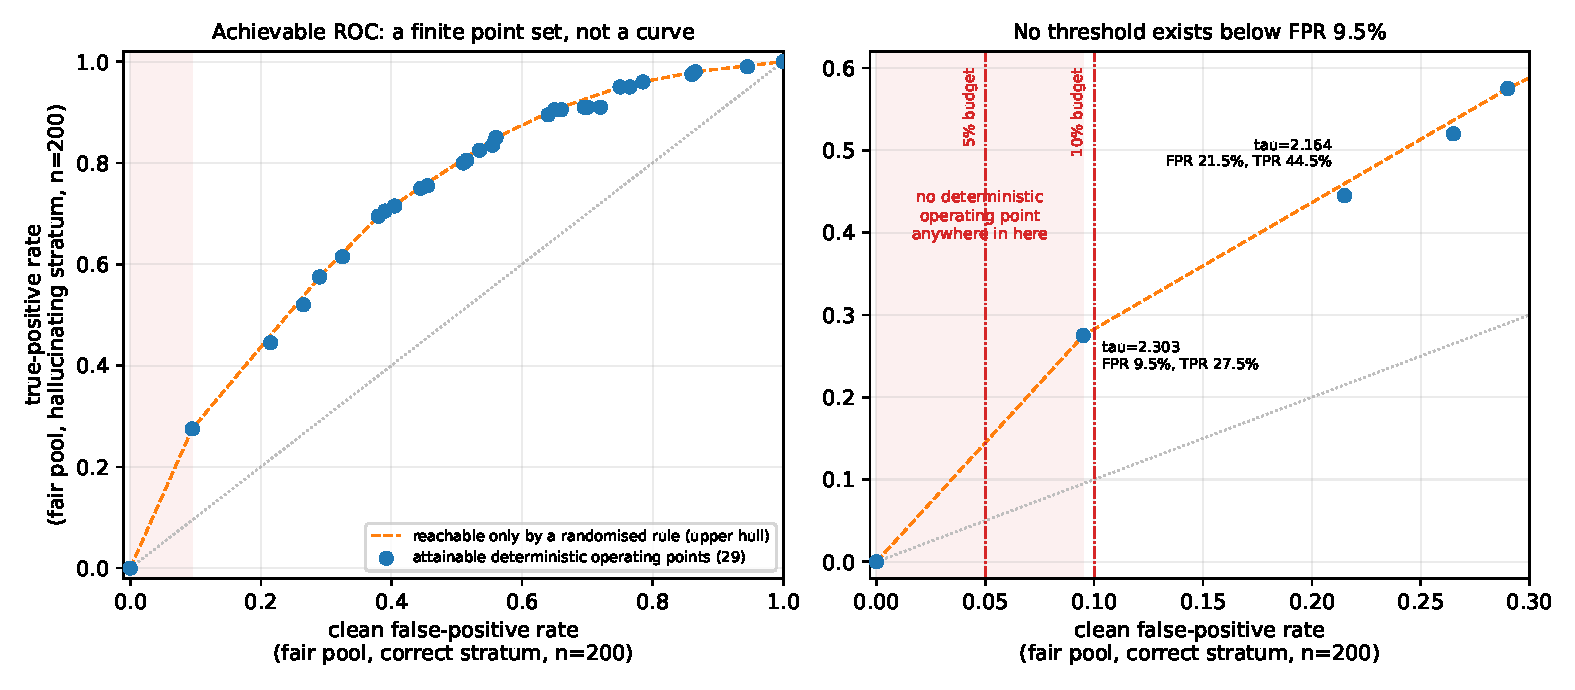
\includegraphics[width=\linewidth]{fig_achievable_roc}
\caption{Every operating point a deterministic threshold on discrete semantic entropy can
occupy at $N{=}10$, on the fair pool's $200$ correct and $200$ hallucinating answers.
Dashed: the upper convex hull. No deterministic threshold exists in the shaded region.}
\label{fig:achievable-roc}
\end{figure}

\paragraph{What this does and does not say about the ROC curve.}
It does not say the ROC curve is fictional, and we state the limit of the claim before a
reader has to. A \emph{randomised} rule flags a ceiling item with probability $p$ and
otherwise never fires. Such a rule reaches any point on the chord between two adjacent
achievable points,
so a $5\%$ false-alarm rate is attainable at $p{=}0.526$, for a true-positive rate of
$14.5\%$ against the $27.5\%$ available at the fair pool's own $9.5\%$ floor. A randomised
rule therefore buys sub-floor false-alarm rates only by paying the average of an indivisible
block. Three things survive that concession. Every \emph{deterministic} operating point,
which is the only kind a deployment can be audited against and the only kind under which the
same input reliably gets the same decision, is one of them (Figure~\ref{fig:achievable-roc}).
On the chord the operator pays the \emph{average} of an indivisible block rather than
selecting its most informative members, which is exactly what the granularity costs. And
randomisation invents nothing below the chord's left end: at any false-alarm rate the
achievable true-positive rate is capped by the upper convex hull of those points, and below
the floor that hull is one straight line out of the origin.

\paragraph{Does a larger sample budget fix it?}
Half of this was settled without data and half needed the measurement, and the two halves
are easy to conflate. Settled without data: the floor is non-increasing in $N$. Couple the budgets by taking the
$N{=}10$ sample to be the first ten draws of the $N{=}20$ one; if all twenty answers are
pairwise inequivalent then so are any ten of them, so $\{\text{saturate at }20\}$ is
contained in $\{\text{saturate at }10\}$, and the first ten of an i.i.d.\ draw of twenty have
the law of an i.i.d.\ draw of ten. Raising the budget can therefore only lower the
false-alarm floor, and the floor itself is a fact about how often the model answers a
question in $N$ ways the clusterer holds apart. That frequency is a property of the model,
the question distribution and the equivalence relation jointly, not of
the estimator's arithmetic. Not settled that way: whether the grid becomes usably
\emph{fine} near the operating region. Enumeration bounds the number of thresholds available in the top tenth of
the range at seven ($455$ attainable values at $N{=}20$, against $39$ and two at $N{=}10$),
but says nothing about the false-alarm rates those seven carry, and that depends on how the
negatives distribute over them. Mass could spread evenly, giving a usable grid, or stay
concentrated on the cap, giving the same pathology one budget along.

We have now run the budget out to $N{=}40$ over the fair pool, recording the full pairwise
equivalence verdicts so that any smaller budget is recoverable by replaying them on random
subsets, and the grid does become fine. Read off that one source, so that no step in the
sequence is also a change of cache, the achievable false-alarm floor on the fair pool's $200$
correct answers falls from a replayed $12.0\%$ [$8.9$, $15.3$] at $N{=}10$ through a replayed
$3.1\%$ [$1.8$, $4.7$] at $N{=}20$ to a measured $2.0\%$ at $N{=}40$, a fall of
$10.0$ points [$7.2$, $12.9$] that excludes zero. That last interval is a paired bootstrap
over the questions and not the two end intervals subtracted, because the two floors are read
off the same $200$ questions and, at $N{=}40$, off a top score that can move to a different
question when those questions are resampled. The ladder is monotone but it is not detectable
at every rung, and we say so rather than let the sequence imply that it is. Taken
leg by leg on the same paired bootstrap, the $N{=}10$ to $N{=}20$ leg is a fall of $8.9$
points [$6.8$, $11.1$], which excludes zero; the $N{=}20$ to $N{=}40$ leg is a fall of $1.1$
points [$-0.2$, $2.4$], which \emph{covers} it. The end-to-end fall is real and its final
increment is not separately resolved at $200$ questions; both belong in the claim, and the
second is the kind of thing this section elsewhere refuses to read a sign off.
Figure~\ref{fig:floor_budget} plots the three budgets and the three paired differences
together. The first two entries are replays of the
$N{=}40$ run's recorded verdicts on random subsets, which is why they are quoted from that
run rather than from the direct Week-4 cache the rest of this paper uses, where the same
$N{=}10$ floor over the fair pool's $200$ correct answers is $9.5\%$ [$6.2$, $14.4$]; the two
paragraphs below are about that difference. The figure shows that direct point separately,
and joins it to nothing, because the June cache it comes from is a different generation run.
Which interval a row takes is decided by the
estimator and not by whether the row was replayed. Wilson prices a count of independent
indicators at a threshold fixed \emph{before} the data, so it belongs to the two rows that
are counts of exactly that kind. Those two rows are the direct $N{=}10$ floor, $19$ of
$200$ at $\ln 10$, and the empty
at-cap mass at $\ln 40$. The replayed rows take a bootstrap over the $200$ questions instead,
because their point estimate is an average over subset draws rather than a count. Those
resample a draw of questions and nothing else; the paragraph below is about why
the replayed rows may not also resample the subset. The measured $N{=}40$ floor takes
neither, for the reason below. What changes qualitatively at the top budget is that the floor stops
being the ceiling atom: no clean correct answer reaches $\ln 40$ at all, so the at-cap mass is
$0/200$, or $0.0\%$ [$0.0$, $1.9$], and the floor becomes an ordinary order statistic. That statistic is
the four
highest-scoring clean answers, $2.0\%$ of the fair pool's correct stratum, at a threshold that
catches $6.0\%$ [$3.5$, $10.2$] of that pool's $200$ hallucinating answers. That is also
why we quote no interval for it. Its threshold is not $\ln 40$ or any
other value fixed in advance but the top score \emph{this} sample attained, and once the atom
is empty nothing in the sample settles whether that score is the top of the population's
support. If it is not, a larger pool reaches a higher rung and reports a smaller floor, so the
quantity being estimated moves with the pool instead of holding still to be estimated; if it
is, the floor is an ordinary population proportion and the count in front of us estimates it.
Nothing here decides which, and the two readings are far apart. Both candidate intervals
inherit that indeterminacy, and each
also has an endpoint placed by construction rather than by the data. A question bootstrap
over these questions cannot return less than $1/200$ however small the floor really is, and
Wilson on a count of four cannot know that the rung it counts may not be the population's
top one. Neither prices the floor, so we report $2.0\%$ as the cheapest alarm $200$ answers
can exhibit and leave it without an interval; what carries one is the at-cap mass above,
whose threshold really was fixed in advance. An empty atom is
not a free operating point, and we separate the two because the arithmetic invites the
confusion: $0.0\%$ is the never-fire policy, and the cheapest alarm that exists at $N{=}40$
costs $2.0\%$.

\begin{figure}[t]
\centering
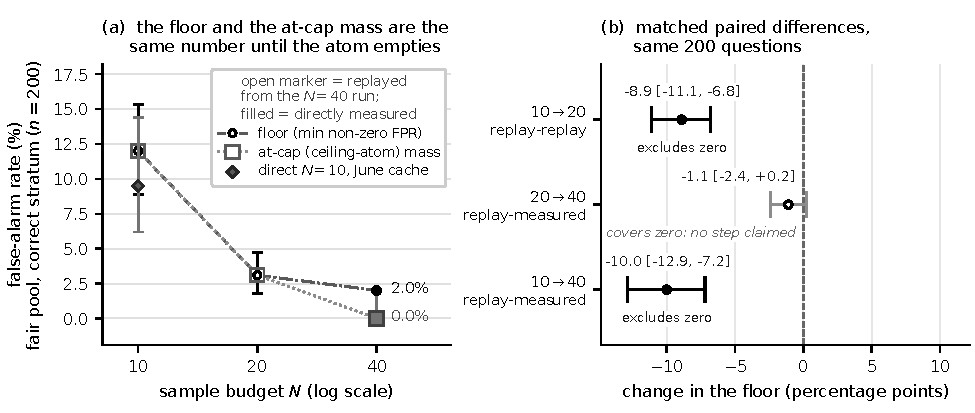
\includegraphics[width=\linewidth]{fig_floor_budget}
\caption{The achievable false-alarm floor on the fair pool's $200$ correct answers against
the sample budget. Left: the floor, and in grey the ceiling-atom mass. Right: the three
matched paired differences over the same $200$ questions.}
\label{fig:floor_budget}
\end{figure}

The grid also densifies where an
operator would use it. At or below a $5\%$ false-alarm budget $N{=}10$ offers no firing
threshold at all, on either source, against five at $N{=}40$; at or below $10\%$ the direct
$N{=}10$ cache offers exactly one, the $9.5\%$ point, against fourteen. So the $5\%$ budget
that $N{=}10$ cannot honour at all is honoured at $N{=}40$, at an achieved $5.0\%$
[$2.7$, $9.0$] on the fair pool's $200$ correct answers. The unqualified form of the claim
above is therefore false and we scope it rather than defend it: the absence of any false-alarm rate
between zero and roughly one correct answer in ten holds \emph{at $N{=}10$} and under this
clusterer, and quadrupling
the sample budget buys the missing operating point.

We report the achieved rate as a measured point and not as a certificate, and we read the
pre-registered criterion on the quantity it was pre-registered on, which is not the one this
paragraph used to compare it against. The plan required a Wilson upper bound below $5\%$ on
the count of correct answers \emph{at the cap}, and derived from that a budget of at most
three such answers in $200$. It identified that count with the floor because at every budget
it was written against, the two were the same number. At $N{=}40$ they came apart: the
at-cap count is $0$, not $4$, its Wilson upper bound is $1.9\%$, and the criterion is met
with three counts to spare. We disclose that reading rather than bury it, because the plan
did not anticipate the atom emptying, and because comparing the four first-firing answers
against a threshold derived for the at-cap count compares two different quantities. That is
the same conflation this work has already had to correct once in the grid report. What the
criterion licenses is narrow and we keep it narrow: the obstruction that closed off a $5\%$
budget at $N{=}10$ is gone at $N{=}40$. That obstruction was an atom of mass at the ceiling,
which no threshold can cut into.
The criterion does not license reading the $5.0\%$ achieved on the fair pool's $200$
correct answers as a demonstration that a
sub-$5\%$ operating point exists, and we do not read it that way. One assumption holds the
certificate up and we state it rather than leave it to be found: that some question in the
population yields $39$ or $40$ mutually inequivalent answers out of $40$ with positive
probability. Were that probability exactly zero, the top of the support would be the rung
this pool reached and the floor would indeed be $4$ of the fair pool's $200$ correct
answers; but $3.1\%$ of them already yield $20$ mutually inequivalent answers out of $20$. The plan priced the remedy in
advance too: thirty further correct answers along
the same seed-$0$ ordering, taken from the larger correct stratum this one is a subset of,
at the pessimistic end of its own predicted floor, with the instruction to trigger the
extension on the measured floor rather than on a hunch. The measured floor triggers it and
we have not run it. So the concession is made at the strength its sample supports. That
strength is five
firing thresholds at or below $5\%$ where $N{=}10$ offers none, and a floor of $2.0\%$ that
we do not certify to sit below $5\%$.
The achieved rate carries the same caution from the other side, since the threshold that
honours the budget is chosen on the same $200$ correct answers whose false-alarm rate it is
then quoted at.

We pre-registered where the claim would break. Before any of these samples were drawn we
predicted, from the $N{=}10$ cache alone, that the ceiling-atom mass would fall to
$3.5$--$5.3\%$ at $N{=}20$ and $1.2$--$2.4\%$ at $N{=}40$; we recorded in advance that the
$N{=}20$ prediction sits on the very $5\%$ boundary this claim turns on, and we committed to
the reversal before the data existed, so that neither branch could be written after the
fact. The plan's own wording was ``if it comes in far below, the finding becomes `here is
the budget that buys a $5\%$ false-alarm rate'\thinspace''.
The branch that fired is the one that was written down, but it fired only at
$N{=}40$, and the prediction that led to it did badly. Both budgets came in \emph{below}
their bands, a replayed $3.1\%$ at $N{=}20$ and an empty atom at $N{=}40$, and the plan had
stated in advance, in bold, that its numbers were lower bounds on the atom and so erred if at
all towards predicting too much relaxation. The pre-registered direction of the error is
therefore itself falsified, which is worth more to a reader than two band misses are. At
$N{=}20$ we claim nothing from the miss, and the reason is narrower than the row's interval
covering the prediction. The row is a replay of an estimator shown unbiased below, but it is
still a replay, and its interval does \emph{not} cover the whole predicted band: it reaches
$4.7\%$, short of the band's top at $5.3\%$, while containing the band's lower edge of
$3.5\%$. So the top of the prediction is excluded and its bottom is not, which is a partial
miss and not the plan's ``far below'': a band whose lower edge survives has not been shown
to be wrong, and a row we have just said may carry no load-bearing claim cannot be turned
into a falsification either. At $N{=}40$ the atom emptied, a $5\%$ operating point appeared,
and the reversal clause is the
one that applies. Even there the band is missed only on the quantity as it was predicted,
since the plan identified the atom with the floor. Read as a floor, the measured $2.0\%$
on the fair pool's correct stratum lands inside the predicted $1.2$--$2.4\%$. The two parted
company exactly when the atom emptied. We give the prediction not as decoration but because
it is what separates a scoped claim from a retreat.

Two limits on this, and neither of them is a bias in the replay. The first is provenance.
Only $N{=}40$ is directly measured; the smaller budgets are \emph{replays} of that run's
recorded verdicts on random subsets, so we route the concession itself through the measured
$N{=}40$ row and let no load-bearing claim rest on a replayed one. That is a rule about where
a number came from, not a doubt about the estimator, which is exactly unbiased for the
smaller budget: the $40$ samples drawn for a question are i.i.d.\ and hence exchangeable, a
uniformly random $k$-subset of an exchangeable $40$-tuple has the law of $k$ i.i.d.\ draws,
and the clusterer is union-find over \emph{pairwise} verdicts, so a subset's clustering is
exactly the clustering a direct $k$-sample run on those samples would have produced. What
reusing one verdict matrix costs is the independence of the replicates and not the mean:
every replicate conditions on the same $40$ samples and the same $200$ questions, so the
spread across replicates is subset-draw noise around a conditional mean. That is a reason to
distrust a sign test taken across replicates. It is not a reason to widen an interval, and
the arithmetic of why is worth setting out, because the mistake is easy to make in the
direction of apparent caution.

The floor a single replicate reports is a mean of independent indicators, one per question,
question $i$ saturating with probability $p_i$ under the subset draw; so its variance splits
as $\overline{p(1-p)} + \operatorname{var}(p) = \bar p(1-\bar p)$, identically. The left term is
the subset draw and the right term is the draw of questions, and their sum is exactly the
binomial variance a Wilson interval on that one replicate already reports. On the fair pool's
$200$ correct answers at $N{=}20$ the two terms, each written as the standard deviation it
contributes to the floor and in that order, are $0.98$ and $0.74$
points against a binomial $1.23$; at $N{=}10$ they are $1.61$ and $1.63$ against $2.30$.
Square-rooted like that they combine as $\sqrt{0.98^{2}+0.74^{2}}$ rather than by addition,
which is the identity above with every term square-rooted and not a sum that fails to
balance. The subset draw is
therefore not missing from a single-replicate interval, and cannot be added to one.

Which interval belongs to which estimator follows. We quote the subset-averaged replay
floor and never a single replicate. That floor is $12.0\%$ at $N{=}10$ and $3.1\%$ at
$N{=}20$, each value the mean of the $200$ per-question
$p_i$ to a Monte-Carlo error under $0.01$ points. The subset-averaged
estimator has the subset draw averaged out of it, so its interval must not put the subset
draw back: what is left varying is which $200$ questions were drawn, each contributing an
independent $p_i$, and a bootstrap over questions is the whole of it. The direct $N{=}10$
row is a count of independent indicators at the fixed threshold $\ln 10$ and takes Wilson;
the measured $N{=}40$ floor is a count at no fixed threshold at all and takes neither, for the
reason given above. The tempting error, and the one this arithmetic rules out,
is to interval the subset-averaged floor by a bootstrap that resamples targets \emph{and}
redraws the subset: that counts the subset draw twice, once inside the target resample where
it already sits and once again in the redraw, and on this data it returns intervals about
twice the width the quoted estimator carries. Widening an interval is not the safe direction
when the interval is the evidence, because it converts a measurable difference into a null.
That is why we state, for every rate in this section, which estimator the interval belongs to.
None of this bears on the unbiasedness argument above: it concerns the width of an interval
and not the location of a point.

The second limit is a provenance question we have not closed. At $N{=}10$ the floor on the
fair pool's $200$ correct answers is $9.5\%$ [$6.2$, $14.4$] measured directly on the Week-4
cache against $12.0\%$ [$8.9$, $15.3$] replayed from the $N{=}40$ run: a step of $+2.5$ points
whose paired interval, $[-0.7, +5.5]$ over the questions,
covers zero. The direct value sits near the fifth percentile of the replay
distribution over $200$ subset draws, which puts it low in that distribution and not outside
it. Subsetting cannot produce
the step, by the argument above, so two candidates remain. Sampling noise in the direct arm is
one: that cache has $19$ of its $200$ correct answers at the $\ln 10$ cap, fewer than the
replay predicts, at an exact one-sided Poisson-binomial $p{=}0.081$, with the rest of the
cluster-count distribution a good fit ($\chi^{2}{=}7.39$ on $9$ degrees of freedom,
$p{=}0.60$). A real difference between the two generation runs is the other, and
one is measurable: the August checkpoint's answers run about $3.6$
characters longer than the June cache's ($z{=}+4.0$) and end in terminal punctuation $1.6$
points less often. What we cannot do is read that drift against a configuration held fixed,
because the two runs' artefacts record only the token budget and the seed in common: past
the model id, its $4$-bit loading, temperature and that budget, the June manifest pins little
of what decides the model's
output. It does not pin the nucleus, the quantisation type or the model revision. The
August checkpoint records nothing of its generation settings at all beyond the sample
count, the token budget and the seed (Section~\ref{sec:limitations}). The drift may be run-to-run variation under configurations
that did match, or a configuration difference we cannot see, and nothing in either artefact
separates the two. Longer and more often truncated answers entail each other less often,
which pushes the ceiling atom up, so the sign is the one the gap would need; how large that
effect is we have not measured, and the cluster-count distribution's failure to separate the
two runs does not bound it (Section~\ref{sec:limitations}). We therefore cannot
separate subsetting error from generation drift, and we claim no direction for the gap. One
clean direct $N{=}10$ pass on the current machine separates them by subtraction. It is one of
two measurements this section is short of, both of them cells the budget plan pre-registered
in advance and neither of them run: this one, a fresh $N{=}10$ pass over $40$ answers of
the correct stratum, and a direct $N{=}20$ pass over $60$ answers of the same stratum. The
second pass asks the other half of this question. Does a replayed grid match a directly
measured one at the same budget?

The one $N{=}20$ re-score elsewhere in this work stands in for none of the above. On $15$
saturated targets re-scored at $N{=}20$, lifting the cap by $0.693$ nats
left $20\%$ of them still pinned and returned a mean of $+0.304$ nats of usable headroom
rather than the full $+0.693$. We report that shortfall without a mechanism for it. The
obvious candidate is that the clean baseline climbs along with the cap, and it is not ours to
offer. A plug-in entropy that rises towards its estimand as the sample grows is that
estimator's negative bias decaying, which is the coverage-adjustment account this paper
cites in \emph{support}~\citep{mccabe2025alphabet, pan2026shade}, and one finding cannot be
both our explanation and their result. The pilot is
a measurement of \emph{headroom}, not of the grid: its $15$ targets were chosen because their
\emph{attacked} $N{=}10$ score hit the cap, which is selection on a score and on the attacked
side, and at that size the interval around the ceiling rate spans almost everything of
interest. It is not evidence about the grid in either direction, and nothing else in this
work is either: no direct measurement of the grid at $N{=}20$ exists. On the fair pool's
$200$ correct answers the trend above reports $3.1\%$ at that budget, and that entry is a
replay of the $N{=}40$ run's recorded verdicts on random $20$-subsets; the only answers this
project has ever scored at $N{=}20$ are the $15$ just described, and they were selected on a
score. The cell that would settle it is the direct $N{=}20$ pass named in the paragraph
above, pre-registered for exactly this purpose and not run.

Under the attack's own success criterion the same coarseness bites from the other side. A
target whose clean score already sits at one of the top two attainable values cannot register
a success whatever the paraphrase: the two lie $0.139$ nats apart, so the criterion's
$\delta{=}0.25$ is out of reach from the lower one and there is nowhere above the upper one
to go, which disqualifies $21$ of the $80$ correct-answer targets of the attack campaign
before any paraphrase is generated (Methods).

The sharpest way to put the finding is therefore not ``we constructed an attack that defeats
semantic entropy'' but ``at the standard $N{=}10$, and under the DeBERTa-large-MNLI
clustering that defines it, discrete semantic entropy offers an
operator no false-alarm rate between zero and roughly one correct answer in ten, and the
false-alarm direction is correspondingly unmeasurable in the detector's own units.'' The two halves are the same fact
seen from the two ends of the deployment, and the first is the stronger form because it is a
statement about what does not exist rather than a frequency we observed. Every qualifier in
it is load-bearing and we drop none of them. \emph{Discrete} carries one: the ceiling behind this reading
is shared with the likelihood-weighted estimator, but the lattice that makes the range so
coarse is not, and the discrete grid of achievable false-alarm rates that comes with it is
not shared either (Section~\ref{sec:methods}). The
first claim invites the reply that a stronger detector, or a stronger optimiser, would settle
the matter. The second does not, because the natural rebuttal is to use an estimator with
more range, and that rebuttal concedes the point. The rebuttal is already being built: coverage-adjusted
estimators exist precisely because the plug-in statistic misrepresents the quantity it
estimates at deployed $N$~\citep{mccabe2025alphabet, pan2026shade}. Whether the remaining, uncensored margin is one an adversary can
reliably exploit is the question the confirmatory evaluation answers. It has now answered it,
and we report the answer with the prominence we promised it whichever way it fell: on the
false-alarm targets the pre-registered exceedance test does not reject in any clusterer arm
(Section~\ref{sec:experiments}). No exploitable margin is demonstrated. That is a statement
about what we can show at this design's power, not a demonstration that none exists, and the
two must not be run together.

That reading also disciplines what we may say about magnitude. Because roughly half of
attacked targets end at the cap, the attack and any other method that also saturates become
indistinguishable there, and effect sizes expressed in nats are censored. The cap bites
asymmetrically. On the fair pool $27.5\%$ of hallucinating answers sit there against $9.5\%$
of correct ones, which is the same pair of numbers as the lowest firing operating point
above, read from the other direction. We are careful not to over-read that. AUROC is a rank statistic and
$\min(\cdot,\log N)$ is monotone, so censoring changes no pairwise ordering except among
pairs where \emph{both} members are pinned. That is $0.275 \times 0.095 = 2.6\%$ of pairs,
bounding the downward bias at $0.013$ against a confidence half-width of $0.050$. The
asymmetry in fact makes the effect \emph{smaller}: had both strata been censored at the
higher of the two rates, $2.9\times$ as many pairs would be affected. The consequence of the asymmetry is therefore about which
class loses resolution, not about the reported AUROC. And because the
reported effect is the maximum over a large candidate search, a further part of it is
selection on estimator noise, and on our own data that part is measurably about half.
Strip both away and
what remains is a modest and heavily conditioned quantity. We think the honest summary is
that whatever margin exists is small, and that most of the apparent margin in an uncorrected
report is an artefact of how the number was obtained. Whether the remainder is real is the
question the confirmatory run decides. It has now run, and it does not decide it in the
attack's favour: the pre-registered statistic does not reject, so, consistent with Methods,
we claim no attack effect here.

\paragraph{Is the weakness structural?}
We conjecture the mechanism generalises beyond one implementation: any detector that
operationalises ``semantic equivalence'' through a learned model inherits that
model's decision boundary as an attack surface. The very component that defines the
score is the component an attacker steers. This \emph{a-priori} argument follows from
the construction alone; the load-bearing \emph{empirical} test is whether the effect
survives an equivalence oracle independent of the detector's own NLI. We run that test.
Cheap independent oracles do not settle it. Exact-match saturates on short factoid
answers, and sentence embedders are near-chance on the adversarial, word-preserving case
(Methods). A victim- and NLI-independent LLM-judge, validated to $0.93$ accuracy on
the gold-alias hard negatives that proxy that adversarial discrimination (where the
embedder scores $0.51$), can settle it for the false-alarm direction, under the disclosed
re-scoped gate (Methods). Under it, the structural question now has an answer for one
direction of one detector, and the answer is negative. An earlier $n{=}6$
machinery-validation sample is evidence about the pipeline rather than about the mechanism:
its interval includes zero, and its per-target diagnostics are too coarse at that sample size
to order the clusterer arms (Methods), so we quote no point estimate from it and draw no
reading either way. The confirmatory run has since completed on all $80$ false-alarm
targets, and the adjudicator's pre-registered exceedance test does not reject
(Section~\ref{sec:experiments}): with the attacker's own search budget priced into the null,
the optimised search does not beat a budget-matched benign one under an equivalence oracle
the detector does not supply. We report that as the gate said we would, and we decline the
stronger form of it. A non-rejection by a design with power $0.77$ against a two-fold effect
bounds what we could have seen, not what exists; it is confined to the false-alarm direction
of the SE detector on those $80$ targets, and it leaves the hide direction and SRE untested.
What the run removes is the licence to claim the effect, not the possibility of one. A single
validated judge, however independent, is in any case not the
last word; SE-to-SRE transfer, confounded by the shared DeBERTa backbone, is at best
corroborating.

\paragraph{The null control's own result is a measurement-validity result.}
The adjudicator arm does not report one number, it reports a family, and the family does not
agree on a sign. Against the mean benign draw the attack's paired net under the LLM judge is
$+0.175$ [$+0.045$, $+0.312$] nats; against the benign candidate selected the same way the
attack's own query was selected it is $+0.016$ [$-0.112$, $+0.150$]; against the best of
$50$ benign candidates ranked on the judge itself it is $-0.173$ [$-0.302$, $-0.039$]. The
attack, the targets and the oracle are identical across those three rows. The only thing
that changes is what the attack is being compared against, and it moves the interval from
excluding zero above to excluding zero below. Not even the top row is a clean win, and we
say so rather than borrow its sign: its bootstrap interval clears zero but its sign test
does not ($p{=}0.44$), because the mean there is carried by a minority of large movers. That
the same data can be read three ways is the point. This is the paper's thesis arriving inside the
paper's own experiment: an attack effect quoted against an unbudgeted comparator is in large
part a statement about the comparator, and the same is true of an attack \emph{deficit}
quoted against an over-budgeted one.

We hold ourselves to that in both directions, which is the part worth saying out loud. The
$-0.173$ is the number a reader most wants us to keep, because it is the number least
flattering to our own attack, and we do not keep it as a finding: the comparator that
produces it is handed a judge-targeted search over $50$ candidates while the attack's judge
score is an unselected re-scoring of a query chosen on the detector's NLI. That is a maximum
compared against a differently-budgeted maximum. It is the exact defect the null control was
built to remove, reappearing one level down, per clusterer arm rather than per design. It
survived because it ran the wrong way: a review looking for bias toward the attack has no
reason to stop on a number that hurts the attack. A validity check with a direction is not a
validity check, and we would not have caught this one by tightening the checklist we already
had. Index-matched, the adjudicator arm cannot be distinguished from zero at $n{=}77$. That
is what we claim. We do not claim the reversal, and we do not claim a win.

\paragraph{Why lead with false alarms.}
Red-teaming of \emph{sampling-based} uncertainty estimators has emphasised the hide
direction (missed hallucinations), though the inflation direction is well established
against other confidence channels~\citep{rusert2025redherring,
khanmohammadi2026answerpreserving}. We foreground false alarms because, for a deployed abstention or
flagging system, systematically inflating the uncertainty of \emph{correct} answers
is its own failure mode: it erodes utility and user trust, and it is cheaper for an
adversary who merely wants to make a model look unreliable. That this \emph{class} of
detector is exposed to it is what would have been new here, and the confirmatory run does not
establish it: the exceedance test does not reject in any arm, so what we contribute in this
direction is the protocol that makes the question answerable and a bound on the effect at this
$n$, not the exposure. The direction itself was not new either.

\paragraph{Defence.}
Averaging the detector score over several reformulations of whatever input is received
should dilute a single adversarial
phrasing, and that averaging is the mechanism SRE already builds in.
We state that expectation as a prediction the experiment can refute. Because the
attacked paraphrase was selected as a maximum over the feasible candidates of a
$\sim$$181$-evaluation search, merely re-scoring it on fresh samples shrinks the effect by
roughly half with no defence of any
kind, so the defended arm has to be measured against a \emph{cost-matched} control that pays
exactly that re-sampling cost and nothing else. That control is a $d{=}1$ fresh redraw of
the same two
inputs. The claim under test is that the per-question paired reduction of the $d$-averaged
arm against that control is positive with a $95\%$ confidence interval excluding zero. Its
failure condition is explicit: if the interval covers zero, reformulation-averaging has
bought the attacker's query cost rather than robustness, and the defence claim is false.
That experiment has not been run. Its arms and its statistic are fixed in advance, and we
report the verdict whichever way it falls. Everything above is to be read against a null noise floor, so that
what we ultimately claim are effects exceeding what benign rephrasing achieves by chance.
That floor has now been measured for the false-alarm direction and is reported in
Section~\ref{sec:experiments}; the defence curve and the SE$\leftrightarrow$SRE transfer are
not covered by it, have not been run, and remain readings of preliminary data rather than
claims.


\section{Limitations}
% Limitations. Draft prose. Owns the construct-validity issues surfaced by our
% own adversarial audit; verify numbers/scope at revision.
\label{sec:limitations}

\paragraph{Our results are scoped to the discrete estimator, and one of them may not transfer.}
We study discrete semantic entropy, for the three reasons given in Section~\ref{sec:methods},
and the paper's claims do not all have the same standing under the likelihood-weighted
estimator that \citet{farquhar2024detecting} designate as their main method. The $\log N$
ceiling transfers by construction: their Eq.~(5) normalises cluster likelihoods into a
categorical distribution over the same at most $N$ observed clusters, so its plug-in entropy
lies in $[0, \log N]$ exactly as ours does. The $39$-point lattice does not: real-valued
weights are not confined to the entropies of integer partitions of $N$, so the exact ties at
the cap, the $0.139$ nats separating the top two attainable values, the unwinnable share of
the false-alarm denominator, and the hard-tie machinery the exceedance test needs all lapse.
Our headline result lapses with them, and we say so plainly. The finite grid of achievable
false-alarm rates, and the floor beneath it, exist because the maximum $\log N$ is an
\emph{atom}. Under real-valued weights it is not one, because Eq.~(5) attains its maximum
only when the normalised cluster likelihoods are exactly equal. Whether a pile-up \emph{near}
the cap would leave a near-atom, and so a near-floor, is a separate empirical question, and
the only part of this we can speak to without the real weights. Our own cached cluster
structure covers the $1424$ greedy-correct questions (alias-aware span oracle, as everywhere
else in this paper) of our $2000$-question replication pass, and with them the $200$-question
correct stratum of the fair pool nested within that set. Re-weighting that structure with
simulated length-normalised likelihoods $\ell \sim \mathcal{N}(0, s^2)$ in place of sample
counts separates two things that ``the pile-up'' runs together
(\texttt{scripts/likelihood\_weight\_sensitivity.py}). The \emph{exact} atom does not
survive: at any positive spread no question sits exactly at $\log N$, and the achievable
floor collapses to $1/n$. That is the measure-zero argument above restated as a measurement
rather than a bracket, and no choice of $s$ rescues it. Near-cap \emph{crowding} does survive
at small spread and decays smoothly: on the fair pool the share of clean correct answers
within $0.05$ nats of the top score is $9.5\%$ at $s{=}0$, still $9.5\%$ at $s{=}0.1$, and
halves by $s \approx 0.46$. What we cannot say is where the real spread falls. Our cache
stores sample strings and not likelihoods, so nothing we have measured constrains $s$ for
length-normalised sequence log-likelihoods from our quantised model on these answers. We
therefore report the curve and decline to claim that its crossover falls inside a plausible
range. Settling it needed the real weights, so we re-scored our stored samples under the
generating model's own sequence likelihoods, on the same questions and the same clusterings,
and computed all three estimators side by side. The simulation's prediction holds and
sharpens. That comparison runs over all $2000$ questions of the replication pass at natural
prevalence, which is the $1424$-answer clean-correct superset above together with its
complement, and not the fair pool. With length-normalised likelihoods the at-cap atom is
\emph{gone}, at $0$ of those $2000$, $0.0\%$ [$0.0$, $0.2$], against $295$ of $2000$,
$14.8\%$ [$13.3$, $16.4$], under the discrete estimator. Near-cap crowding partially
survives, at $399$ of $2000$, $20.0\%$ [$18.3$, $21.8$] in the top tenth of the range against
$556$ of $2000$, $27.8\%$ [$25.9$, $29.8$]. The atom, and therefore the false-alarm floor it
induces, is a property of sample-proportion weighting; the crowding is not. Length
normalisation is the choice doing that work: on raw sequence likelihoods the cluster softmax
is nearly one-hot and rank agreement with the discrete estimator collapses to $\rho{=}0.38$,
whereas length-normalised it is $\rho{=}0.99$, and on the score-independent fair pool ($200$
correct, $200$ hallucinating) it scores AUROC $0.703$ against the discrete estimator's
$0.704$. Every AUROC in this paper therefore stands under Eq.~(5) as we compute it, and only
the saturation arithmetic is estimator-specific.

\paragraph{One cached generation run underlies every $N{=}10$ number here.}
The re-scoring above, the achievable false-alarm floor and its grid, the clean AUROC on the
fair pool, and the corresponding floor on the $1424$-answer superset are all computed from a
single cached pass of $N{=}10$ samples over $2000$ TriviaQA validation questions, generated in
June 2026. Two properties of that cache bound what any of them establishes, and neither is
visible in the numbers themselves.

First, the run is under-recorded. Its manifest pins the model id, $4$-bit loading, the sample
count, temperature $1.0$, a $48$-token generation budget, the seed and the split, and of the
settings that determine what the model emits it pins nothing further: not \texttt{top\_p}, not
the $4$-bit quantisation type, not whether double quantisation was applied, not the compute
dtype, not a model revision, and not the \texttt{transformers} version. Those six values are
recovered from the defaults of the sampling script's own source rather than read off the
artefact. This paper quotes none of them as a property of the June run, and a later draft
should not start. Exactly one place in this project has a value for any of them on record, the
\texttt{top\_p}${=}1.0$ in the $N{=}40$ run's own provenance block. That block describes the
August generation pass and says nothing about this cache. The absent revision hash is the one
we would most like back: without it we cannot certify that a re-run today would load the same
weights. A further gap is structural. The cache stores decoded answer strings and never the
token ids the sampler emitted, so the likelihood re-scoring teacher-forces each answer under
its \emph{canonical} tokenisation; $17$ of the $20{,}000$ cached samples ($0.085\%$) retokenise
past the $48$-token budget, which proves the two id sequences differ for at least those, and
the detokenise-then-retokenise string round trip itself is exact for only $19{,}996$ of the
$20{,}000$, its four failures all trailing whitespace. Both figures are lower bounds, since a
resegmentation that preserves the token count leaves no trace in either check, so what Eq.~(5)
recovers above is the likelihood of each answer \emph{string} under its canonical tokenisation
rather than of the sequence the model emitted.

Second, generation runs of this pipeline are not interchangeable, and we have measured that
they are not. The August $N{=}40$ run, drawing fresh samples for the same fair-pool questions,
produces answers about $3.6$ characters longer ($z{=}+4.0$) that end in terminal punctuation
about $1.6$ points less often; the two runs' artefacts record only the token budget and the
seed in common, so we cannot certify that the rest of their configurations matched either. We
disclose that drift in Section~\ref{sec:discussion}, where it bears on a comparison between the
two runs. It bears on every June-cache number in this paper as well, and we have not bounded it
for any of them. The statistic that would carry it into them is the distribution of the cluster
count at $N{=}10$, which is the whole of what the discrete score is a function of, and on the
fair pool's $200$ correct answers that distribution is not distinguishable from what the August
run's recorded verdicts predict for it. We decline to read that as a bound: a comparison on
$200$ questions that fails to separate two runs is not a measurement of how close they are, and
treating it as one is the move this paper has had to retract elsewhere. One fresh direct
$N{=}10$ pass on the current machine separates drift from sampling noise by subtraction, and we
regard it as owed.

\paragraph{Selection on a noisy estimator, measured rather than merely acknowledged.}
Semantic entropy is a finite-sample quantity: for each candidate we cluster $N{=}10$ sampled
answers, so the score is a Monte-Carlo estimate of the true entropy. Our optimiser selects the
extremum of this estimate over $\sim$180 candidate paraphrases, and the extremum of many
noisy-but-unbiased estimates is biased in the attacker's favour even when, as here, sampling is
seeded so each estimate is \emph{reproducible}. Reproducibility is not the same as
noise-freeness.

We quantify the resulting inflation directly, by re-scoring each \emph{selected} paraphrase on
an independent sample at the same $N$ under a different sampling seed. That is the classical
diagnostic for selection on noise, and it requires neither an oracle nor a benign floor. The
re-scored set is the $69$ of the $80$ false-alarm targets on which the optimiser found a
paraphrase at all; on the other $11$ the search returned the original question, so there was no
selection to re-test. Across those, the mean intended move falls from $+0.609$ nats at
selection to $+0.268$ nats on fresh samples. Two statements follow, with very different
strengths, and we separate them. \emph{That} the selection-time figure is inflated is
demonstrated: the shrinkage is $-0.341$ nats with a bootstrap interval of $[-0.469, -0.212]$
that excludes zero. \emph{How much} it is inflated is not tightly determined: retention is a
ratio of means, and its interval is wide at $44\%$ $[23\%, 64\%]$. So roughly half of the
effect a naive report would claim is selection on sampling noise rather than a property of the
paraphrase, but the honest range runs from under a quarter to two-thirds surviving. Signal
remains either way, since $37$ of the $69$ keep a positive move and the two measurements
correlate at $r{=}0.48$.

We therefore do not report raw effect sizes as the headline. The claim statistic prices the
attacker's search budget into the null (Section~\ref{sec:experiments}), so an effect that does
not exceed what a benign search of comparable size achieves by chance is not claimed. We note
that this re-scoring diagnostic bounds only the \emph{selection} component: it says nothing
about whether random rephrasing achieves the same move, which is the separate question the null
control answers.

\paragraph{The clusterer and the equivalence gate share one NLI model.}
Semantic entropy is \emph{defined} by DeBERTa-large-MNLI bidirectional clustering, and our
attack's feasibility constraint uses the same model, so a measured degradation could in part
reflect that one model's self-inconsistency rather than a paradigm-level weakness. We address
this directly by re-clustering the answer samples under equivalence oracles independent of the
DeBERTa-MNLI supervision (Methods), but two caveats bound the check. First, the cheap
independent oracles are unreliable on the adversarial case (exact-match saturates; the sentence
embedder is near-chance), so the adjudication rests on a single LLM-judge. That judge is
validated ($0.93$) on the hard discrimination the others fail, but a single oracle is not
dispositive even when it is independent and validated, and a human or multi-judge equivalence
audit remains owed. Second, the judge's own positive-recognition is imperfect, at $0.65$
[$0.59$, $0.70$]. On the clean gold-alias pairs it was validated on, it \emph{over}-splits
genuine aliases, in part correctly rejecting noisy TriviaQA alias labels. The pre-registered
conservativeness argument for the false-alarm direction was built on that behaviour.
Over-splitting inflates the clean baseline, so a surviving false-alarm effect is understated.
\textbf{That argument does not survive contact with this campaign's own data.} On the messy
sampled answers the deployed judge actually clusters, it \emph{under}-splits: over the $80$
false-alarm targets its mean clean baseline entropy is $0.648$ nats against the NLI clusterer's
$1.477$, and it collapses all ten samples into a single cluster on $27$ of the $80$ clean
baselines where NLI does so on $4$. Both statements are true, each of a different input. The
judge over-splits clean alias pairs, and it under-splits sampled answers. The second behaviour
is the one that governs the numbers we report, so we do not carry the first forward as though
it settled the direction of the bias. The consequence runs the other way from the
pre-registered worry: a floored baseline bounds the measured false-alarm move below by zero on
those $27$ targets, which is anti-conservative for a false-alarm claim rather than
conservative. We disclose it rather than correct it, because we did not make a false-alarm
claim: dropping the floored targets leaves the judge-arm move at $+0.247$ [$+0.072$, $+0.429$]
nats against $+0.291$ [$+0.152$, $+0.440$] on all $80$, and the adjudicator's exceedance test
does not reject either way. The independent-clusterer result is reported as the confirmatory
$n{\geq}80$ run's own result and no longer as preliminary evidence; what remains preliminary is
the merge-side bias estimate, which the planned validation was designed to be blind to and
which is owed before any judge-arm effect size is claimed.

One consequence of that shared dependence reaches past the attack and into the
measurement-validity result, and we had not scoped it far enough. The achievable false-alarm
floor we report is the mass of an atom at $\log N$, and what sits at $\log N$ is whatever the
clusterer declines to merge, so the floor is a property of this clusterer as much as of the
model. Section~\ref{sec:discussion} measures how far it moves when the relation is changed
and the samples are held fixed: on one set of $80$ clean targets the same estimand reads
three different ways, and the exact-match and NLI intervals do not overlap. Every floor claim
in this paper is therefore scoped to bidirectional DeBERTa-large-MNLI clustering. We do not
claim the converse, that a more permissive relation delivers a usable low false-alarm rate,
because the one relation that would suggest it is measured at a denominator too small to
exclude the budget in question.

\paragraph{Equivalence is certified automatically, not by humans.}
Feasibility is a judgement of bidirectional entailment. Our answer-flip subcategory collects
the successful attacks in which the model's correctness flips under $q'$, and that subcategory
is a \emph{lower} bound on how often the gate admits a non-equivalent paraphrase, since a $q'$
can shift scope or presupposition while leaving the greedy answer unchanged. We do not yet
report a human (or disclosed strong-LLM-judge) equivalence audit of a random sample of
successful $q'$; such an audit, with an inter-annotator agreement estimate, is needed before
the meaning-preserving claim is fully established.

\paragraph{Status check versus what the detector sees.}
The success criterion re-checks the model's answer with a single greedy decode, while the
detector clusters temperature-$1.0$ samples. The two can disagree, because a greedy answer may
stay wrong while the sampled distribution shifts toward correct (or vice versa). We therefore
report both the greedy status and the fraction of the detector's own samples that are correct
under $q'$, rather than relying on the greedy check alone.

\paragraph{Model, precision, data, and budget.}
Results are on a single model family (Llama-3.1-8B-Instruct) run in 4-bit quantisation on one
16\,GB GPU; quantisation may shift both the entropy estimates and the attack surface relative
to a full-precision detector, and generalisation across model families and scales is untested.
Our primary dataset is TriviaQA; broader datasets (e.g.\ SQuAD) are in progress. The attack
budget (beam and iteration counts) is modest by necessity, and the reported cells use small
per-stratum $n$, so the confidence intervals are wide and the numbers are best read as
preliminary effect sizes rather than tight estimates.

\paragraph{One measured sample budget, and how coarse the ladder is.}
The budget in the paragraph above is the \emph{attacker's} search budget; this one is the
detector's sample budget $N$, and the scope limit we draw from it needs stating in its own
right. The achievable false-alarm floor falls as $N$ rises, so that the absence of any low
false-alarm operating point is a fact about $N{=}10$ and not about semantic entropy. That claim
rests on a single directly measured budget. We ran $N{=}40$ once, over the fair pool's $400$
targets, $200$ per stratum. The $N{=}10$ and $N{=}20$ rows of the falling sequence are not
further experiments: they are replays of that one run's recorded pairwise equivalence verdicts
on random subsets of its $40$ samples, unbiased for the smaller budget by the exchangeability
argument of Section~\ref{sec:discussion}, but read off one generation run rather than three.
Only the top of the ladder is a measurement and nothing above it was run, so what we can say is
that the floor is non-increasing in $N$, which we prove rather than measure, and that on the
fair pool's $200$ correct answers it had reached a measured $2.0\%$ by $N{=}40$; how it behaves
further out, and whether the decay between two coupled points is the shape it keeps, we cannot
say. Three narrower scopes ride along. The ladder exists only on the fair pool. The
$1424$-answer superset estimates the same $N{=}10$ floor as the fair pool's $9.5\%$ over seven
times as many negatives, but it has no $N{=}40$ counterpart, so every row here is estimated on
$200$ negatives, a resolution that cannot separate false-alarm rates less than half a point
apart. It is one model family in one quantisation on one dataset read through one equivalence
relation, and the floor is a fact about how often that model answers a question in $N$ ways
the clusterer holds apart, a property of the model, the question distribution and that
relation jointly rather than of the estimator's arithmetic, which is exactly the kind of
quantity that need not transfer to another model, another corpus or another notion of
sameness. And what the extra
operating points are \emph{worth} we do not report in either direction: at a matched
false-alarm rate the cross-budget change in true positives has a magnitude that depends on
which decision rule is paired and a sign that depends on which $N{=}10$ cache is paired, and no
pairing separates the budgets on $200$ questions, so we claim no discrimination benefit from a
larger budget and, equally, none against one.

\paragraph{SRE fidelity and threat model.}
We reproduce SRE with exact-match-then-NLI-union-find clustering rather than the paper's full
energy-based hybrid, and our NLI backend (deberta-large-mnli) is weaker than the
deberta-v2-xlarge used in some prior work; the SRE target (paper $0.871$) depends further on
the clustering backend we simplified. Our \emph{SE} replication reaches AUROC $0.694$ under the
greedy alias-aware span oracle this paper operates with, against the paper's SE figure of
$0.828$. We do not attribute that $0.134$ gap to the backend. The nearer-looking $0.790$ is the
same run scored under an all-samples-correct label, a convention mechanically coupled to
semantic entropy that we use nowhere else (Section~\ref{sec:experiments}); backend and
correctness convention are thus confounded in the gap, and separating them needs an ablation we
have not run. Because SRE re-paraphrases its input internally, the attacker's chosen $q'$ is
only one input to a detector that then generates its own reformulations; the SRE threat model
(whether the attacker controls the reformulation set) needs to be stated and matched to the
implementation, which we flag as a limitation of the SRE results specifically.

\paragraph{Our novelty claims carry a documented search gap.}
Every ``to our knowledge'' in this paper is bounded by a coverage limit we can state precisely.
We searched the public arXiv record, ICLR 2026, TMLR under-review, six ARR cycles, and the COLM
and ICML workshop tracks. We could not search the NeurIPS 2026 main track, the ARR February,
June and July 2026 cycles, the COLM 2026 main track, or the full text of any OpenReview
submission. For those three ARR cycles the indices return zero results to control queries that
return hits for neighbouring cycles, so we have verified the index is empty rather than merely
finding nothing. Absence of hits from those venues is therefore \emph{uninformative}, not
weakly reassuring, and we do not treat it as evidence. The relevant pace: the closest
concurrent work we identified had been public for six days when we found
it~\citep{khanmohammadi2026answerpreserving}.


\section{Conclusion}
% Conclusion. Framing stable; keep claims scoped to null-controlled evidence.
%
% "Fill the final effect size at revision" USED TO STAND HERE AND IS RETIRED. The effect
% sizes are filled: the run completed 80/80 on 2026-08-29 and every figure below is the
% landed one. Leaving that instruction in place would have invited the next editor to
% overwrite measured numbers, which is the defect class the Abstract's comment block calls
% "a comment does not merely record an error, it schedules one".
%
% TWO SCOPE QUALIFIERS ARE LOAD-BEARING IN THIS FILE AND NEITHER IS DECORATION.
%  (a) N=10. The 5%-budget exclusion is true at N=10 and false at N=40; the file concedes
%      that in the same paragraph.
%  (b) The clusterer. Added 2026-08-30 under item M1 of results/gemini_adjudication_
%      2026_08_30.md. The same estimand reads 46.2% / 10.0% / 1.2% across exact match, the
%      NLI clusterer and the judge on one fixed set of samples, so an unscoped floor
%      under-specifies its own estimand. The canonical long form used across the paper is
%      "bidirectional DeBERTa-large-MNLI clustering"; Discussion carries the three numbers
%      and the factor, this file carries the scope only.
%
% THE NON-REJECTION RESTS ON THE ADJUDICATOR ARM, NOT ON ALL THREE. The sentence "in every
% clustering arm, and at every one of 101 tie-break draws ... the median observed exceedance
% count sits above its null expectation" was DELETED on 2026-08-30 and may not come back.
% Both halves are conditional on the search budget A being 181, A is only bounded above by
% what the run recorded, and the shared-NLI arm's p crosses 0.05 inside the admissible range
% (experiments.tex has the range and the sensitivity rows). The adjudicator arm is invariant
% across that range, which is why the verdict is drawn from it.

Sampling-based hallucination detectors treat semantic uncertainty as a property of the
question, invariant to surface form. We set out to test that assumption adversarially and
found that the more informative obstacle lay upstream of the adversary, and that it is
sharpest stated as a constraint on the operator rather than on the attacker. At $N{=}10$ the
\emph{discrete} estimator we study is confined to a lattice of $39$ attainable values with
an atom at the maximum, so a detector that flags when the score reaches a threshold can be
run only at a finite list of false-alarm rates. Scored clean on the fair pool's $200$
correct answers, the achievable rates below one in four are $0\%$, $9.5\%$ [$6.2$, $14.4$]
and $21.5\%$, catching $0\%$, $27.5\%$ and $44.5\%$ of that pool's $200$ hallucinating
answers. An operator who specifies a $5\%$ false-alarm budget cannot have one at that sample
budget, because the only threshold that honours it never fires. That floor is an identity
rather than a measurement for as long as the cap carries mass, since every threshold above
$\ln N$ flags nothing and the smallest rate a firing threshold can have is therefore the
mass of the ceiling atom itself. That mass is the probability that a clean correct answer
yields $N$ mutually distinct meanings, which the $1424$-answer superset puts at $10.5\%$
[$9.0$, $12.2$]. At $N{=}10$ a $5\%$ budget is excluded at $95\%$ confidence on both
populations; a $10\%$ budget is on the boundary and we claim no more than that. The
qualifier is load-bearing: measured out to $N{=}40$ over the same $200$ correct answers the
cap carries no mass ($0.0\%$ [$0.0$, $1.9$]), the floor ceases to be an identity and becomes
an ordinary order statistic at $2.0\%$, and the threshold that honours a $5\%$ budget
achieves $5.0\%$ [$2.7$, $9.0$] on that same correct stratum of the fair pool. We report the
second as a measured operating point and not as an existence claim, and we attach no
interval to the first: its threshold is the top score \emph{these} $200$ answers happened to
reach, so $2.0\%$ is the cheapest alarm a pool of this size can exhibit rather than an
estimate of how cheap an alarm can be. What the pre-registered criterion asks for is a
one-sided bound on the mass \emph{at the cap}, and that bound is the $1.9\%$ above, which
falls under the line rather than over it (Section~\ref{sec:discussion}). A second qualifier
is load-bearing in the same way, and it names the clusterer rather than the budget.
``Mutually distinct'' is whatever the equivalence relation says it is, and on the same
attacked targets and the same clean samples the mass at the cap moves by more than an order
of magnitude as that relation is varied from exact match to the detector's NLI clusterer to
the independent judge, the exact-match and NLI intervals not overlapping
(Section~\ref{sec:experiments}). The floor we report is accordingly the floor under the
bidirectional DeBERTa-large-MNLI clustering the detector ships, and what we claim across
relations is that dependence itself rather than a floor surviving all of them. The claim is about
deterministic rules: a randomised rule reaches the chords between these points, but only by
paying an indivisible block's average, and below the floor the reachable frontier is a
single chord out of the origin. The $\log N$ ceiling behind all of this is shared with the
likelihood-weighted estimator its authors designate as their main method. The lattice, and
so the grid of achievable false-alarm rates, is particular to the discrete variant that the
same authors run for their GPT-4 results and that semantic entropy probes are trained to
predict. This is not a claim that the detector fails. On the score-independent \emph{fair}
pool ($200$ correct, $200$ hallucinating) it separates correct from hallucinating answers
moderately well, at AUROC $0.704$ [$0.653$, $0.753$]. That fair pool is the wider population
on which we characterise the detector, and the one our targets are a sub-sample of. The
claim is instead that at $N{=}10$ the region where a false alarm lives is compressed to the
point where an operator has no usable choice inside it, and differences there are largely
unmeasurable in the detector's own units.

Establishing even that much honestly turned out to require more care than the question first
appears to need. Because the attack reports a maximum over a large candidate search, about half
of its apparent effect is selection on estimator noise, which we measure directly by re-scoring
the selected paraphrase on independent samples. Because the score saturates, effect sizes in
its native units are censored on just over half of attacked targets, and a null must remain
valid when attack and benign candidates tie at the cap. And because the detector's clusterer is
the same model that certifies our paraphrases as meaning-preserving, no single-clusterer
measurement can separate a real change in the model's answers from that model's own
inconsistency. The confirmatory evaluation was run under a protocol built to survive all three.
Targets were chosen without reference to the detector's own scores, success required the
hallucination status to survive the paraphrase, and the null prices the attacker's search
budget in rather than comparing a maximum against single draws. We confine claims to what that
protocol supports, and on the evidence it returned that is no attack effect. The
pre-committed exceedance test fails to reject in every clustering arm. We draw that verdict
from the pre-registered adjudicator arm rather than from the shared-NLI one, and the reason
is a limit of our own instrumentation rather than a preference: the search budget the null
prices in is the number of candidates the attack's equivalence gate admitted, the gate was
applied lazily, and the run recorded enough to bound that number from above but not to
identify it. The shared-NLI arm's $p$-value is sensitive to where in that range the true
budget lies. The adjudicator's is not, and it does not reject anywhere in it.

Two boundaries remain, and we state them as the work to do rather than as caveats to wave away.
First, our clusterer and our equivalence gate are the same NLI model, so whether the
vulnerability is a property of the \emph{paradigm} or of one model's self-inconsistency turns
on an independent clustering oracle. We build one. The cheap candidates (exact match, sentence
embeddings) fail on the adversarial case, but a victim- and NLI-independent LLM-judge,
validated on a domain-matched proxy of that case ($0.93$ vs.\ $0.51$), clears it. It is under
this judge that the confirmatory large-$n$ run, now complete, adjudicated whether the
false-alarm effect survives the independent clusterer (the direction to which the judge is
re-scoped; Methods). It does not survive it: the adjudicator's exceedance test does not reject,
and index-matched against a benign candidate selected the same way the attack's own query was,
the adjudicator arm cannot be distinguished from zero ($+0.016$ [$-0.112$, $+0.150$] nats).
That is the verdict we draw from that run rather than from the machinery-validation sample, and
it bounds the effect we could have seen at this sample size rather than excluding one. Second,
the meaning-preserving guarantee rests on an automatic gate; a human equivalence audit is
needed before it is fully established. Whether a simple reformulation-averaging defense confers
measurable robustness is an open question we frame but do not yet settle. The experiment is
specified and has not been run. We have specified it so that it can fail: the $d$-averaged arm
must beat a cost-matched $d{=}1$ fresh-redraw control by a per-question paired margin whose
$95\%$ interval excludes zero, and an interval covering zero means the defense bought the
attacker's query cost rather than robustness. Taken together, the results argue that
``semantic'' uncertainty inherits the blind spots of whatever model defines its notion of
meaning. They also argue that detectors built on a learned equivalence relation should be
evaluated as the adversarial targets they now are.


% DATA AND CODE AVAILABILITY. Added 2026-08-31; there was none before. The review of
% 2026-08-30 (results/heavy_review_2026_08_30.md, F7) grepped the whole PDF and all seven
% section files for availab|github|repositor|artifact|licen|zenodo|url|http|href|doi.org|
% acknowledg and found only package options and unrelated prose ("sequence probabilities are
% not available"). For a paper whose contribution is measurement validity, and whose
% Limitations rest it on one under-recorded generation cache, that is among the first things
% a referee checks, and ARTIFACT_AVAILABILITY.md says so in its own opening: "Adding an
% availability statement to the paper is a separate, owed edit; this file does not
% substitute for it."
%
% EVERY CLAIM BELOW WAS CHECKED AGAINST THE TREE ON 2026-08-31, NOT AGAINST A SUMMARY OF IT:
%   - the URL is what `git remote get-url origin` returns and what README.md's own citation
%     block prints;
%   - LICENSE is tracked, MIT, "Copyright (c) 2026 ScriptSampler". It covers the CODE. The
%     data bundle's licence is UNDECIDED (ARTIFACT_AVAILABILITY.md section 6 item 3: the
%     cache carries TriviaQA questions and Llama-3.1-8B-Instruct generations, whose
%     redistribution is not self-evidently MIT), which is why this paragraph licenses the
%     repository and says nothing about a data licence. Do not add one until it is decided;
%   - what a bare clone reproduces is ARTIFACT_AVAILABILITY.md section 2, which verified it
%     by running it on CPU with no cache present, and figures/ does carry a plotted-points
%     CSV for each of the paper's four figures (fig1_ceiling, fig2_censoring,
%     fig_achievable_roc, fig_floor_budget);
%   - the 4.75 MB is wk4_full_2000q, measured file by file in section 3.2.
%
% NO COMMIT HASH IS PRINTED, AND THAT IS DELIBERATE. F7's fix asks for "a URL and a commit
% hash". This edit is uncommitted, so any hash written here would name a state that predates
% the statement itself and would be stale the moment it landed. Fill it with the submission
% commit before any external posting, on the same schedule as the affiliation above, and do
% not ship a placeholder in its place.
%
% DO NOT UPGRADE THE WORDING. "is not currently distributed", "cannot re-run the pipeline
% that produced them" and "we claim no more reproducibility than that" are the honest form
% and were chosen over stronger ones. The cache is 4.75 MB, so what stands between a reader
% and the empirical half is a decision not yet taken, not a technical obstacle; a sentence
% implying the numbers are rebuildable from a clone would be the one overclaim in a paper
% whose stated virtue is that it does not overclaim.
\section*{Data and Code Availability}
Code, analysis scripts, the dated reports of record that own the numbers above, and the
plotted points behind every figure are in the repository, under the MIT licence:
\begin{center}
\url{https://github.com/ScriptSampler/red-team-semantic-entropy}
\end{center}
\noindent
What a clone buys differs sharply between the two halves of the headline, and we would rather say
so than let a URL imply more than it delivers. The combinatorial half reproduces from a bare
clone with no data, no model and no GPU: the $39$ attainable values at $N{=}10$, the two of
them in the top tenth of the range, the atom at $\ln 10$, and the corresponding counts at
$N{=}20$ and $N{=}40$ are an enumeration over integer partitions, pinned on CPU in seconds
against an independent implementation. The read-only checkers that verify the population
label on every rate we print, and that re-derive the printed quantities with no producing
artifact of their own, run in a fresh clone as well. The empirical half does not. Every
measured rate here is computed from a sample cache of $2000$ TriviaQA \texttt{rc.nocontext}
questions with ten Llama-3.1-8B-Instruct generations each, $4.75$ MB, which lives outside the
repository tree and is not currently distributed; the null control's per-target checkpoints
are written into the tree and then excluded from it. A clone therefore carries every derived
report and each figure's plotted points as a CSV, so the arithmetic is auditable from the run
outputs onward, but it cannot re-run the pipeline that produced them, and we claim no more
reproducibility than that. \texttt{ARTIFACT\_AVAILABILITY.md} in the repository names the
files a clone is missing, with their sizes and SHA-256 digests. Model weights and datasets
are obtained from their upstream sources under their own licences and are not redistributed
here.

\bibliographystyle{plainnat}
\bibliography{related_work}

\end{document}
